%% learnheuristic_pmsp.tex
%% Compilar: xelatex -> bibtex learnheuristic_pmsp -> xelatex -> xelatex
%% Migrado para a classe elsarticle (Elsevier) na Entrada 76 (08/09/2026)
%% -- exigencia do EJOR (ver ANALISE_E_PLANO_EJOR.md, Secao 4). elsarticle.cls
%% e elsarticle-harv.bst (citacao estilo Harvard/autor-ano, pedido do EJOR)
%% vem junto deste arquivo, na mesma pasta -- nao fazem parte de nenhuma
%% instalacao TeX Live padrao (pacote texlive-publishers, confirmado ausente
%% tanto no ambiente de Carlos quanto no de verificacao).
%% Opcoes da classe atualizadas na Entrada 85 (09/09/2026, Task #45) para
%% bater exatamente com o artigo irmao do LCPP (Amaro Junior et al., em
%% preparacao para o EJOR, mesmo grupo/coautoria de Carlos): [final,3p]
%% no lugar de [preprint,review] -- decisao explicita de Carlos, coluna
%% unica em largura "de producao" (mais estreita que o preprint largo),
%% sem numeracao de linha de revisor. [times] ativa txfonts (Type 1,
%% compativel com xelatex sem fontspec) em vez da Computer Modern padrao,
%% [11pt] no lugar de [12pt] -- ambos tambem para bater com o LCPP.
%% \onehalfspacing (pacote setspace) e' carregado explicitamente depois
%% da classe pra manter 1.5 espaco mesmo com [final] (que por si so'
%% forcaria espaco simples) -- mesmo padrao usado no LCPP, apropriado
%% enquanto o artigo ainda esta' em fase de rascunho/revisao interna.
%% [authoryear] ativa a citacao estilo Harvard via natbib (\citep/\citet),
%% carregado automaticamente pela propria classe -- nao precisa de
%% \usepackage{natbib} manual.
\documentclass[final,3p,times,11pt,authoryear]{elsarticle}

\usepackage[utf8]{inputenc}
\usepackage[T1]{fontenc}
\usepackage{amsmath,amssymb,amsfonts}
\usepackage{graphicx}
\usepackage{textcomp}
\usepackage{subcaption}
\usepackage{booktabs}
\usepackage{longtable}
\usepackage{multirow}
\usepackage{url}
\usepackage{float}
\usepackage{algorithm}
\usepackage{algorithmic}
\floatstyle{ruled}
\restylefloat{algorithm}
\usepackage{setspace}
\onehalfspacing
\usepackage{enumitem}
\setlist{nosep,topsep=2pt,itemsep=1pt,parsep=0pt,leftmargin=*}
\setlength{\textfloatsep}{8pt plus 2pt minus 2pt}
\setlength{\floatsep}{6pt plus 2pt minus 2pt}
\setlength{\intextsep}{6pt plus 2pt minus 2pt}
\setlength{\abovecaptionskip}{4pt}
\setlength{\belowcaptionskip}{2pt}
\usepackage{xcolor}
\usepackage{bm}

\sloppy

\journal{Journal of Heuristics}


%% supplementary_material.tex -- material suplementar (Entrada 95).
%% Contem o capitulo `ils_ql` e a exploracao de mecanismos hibridos IG/ILS,
%% movidos do corpo do artigo para respeitar o limite de 30 paginas do EJOR.
%% Referencias cruzadas ao artigo principal via pacote xr (compile o artigo
%% principal primeiro, depois este arquivo, depois o principal de novo).
\usepackage{xr}
\externaldocument{learnheuristic_pmsp}
\renewcommand{\thesection}{S\arabic{section}}
\renewcommand{\thetable}{S\arabic{table}}
\renewcommand{\thefigure}{S\arabic{figure}}
\renewcommand{\theequation}{S\arabic{equation}}

\begin{document}
\begin{frontmatter}
\title{Supplementary material for: \emph{Mechanism or policy? Budget-fair attribution of the gains of
       learning-guided metaheuristics in scheduling}}
\author{Carlos Vinicio Dantas Ara\'{u}jo}
\address{Graduate Program in Computer Science, State University of Cear\'{a} (UECE), Fortaleza, CE, Brazil}
\begin{abstract}
This supplement collects the parts of the study that the main text summarises but does not reproduce:
the details of the experimental design (state, Iterated Greedy components, instances and methods);
the full comparisons of the Q-Learning-guided IG with the ILS family and the published baselines, the
stronger baselines and the exact reference for identical machines; the robustness analyses of the
policy effect (state, reward, hyperparameters, seeds, budget); the recipe with a local search at equal CPU
time; the full external validation; the granularity of the processing times and the dispatch rule; the
synthetic unrelated-machine experiments; the companion \texttt{ils\_ql} study; a preliminary exploration of
hybrid IG/ILS mechanisms; further robustness experiments; the certified lower bound; and the record of all
pre-specified analyses.
\end{abstract}
\end{frontmatter}
%% Auto-generated by paper/make_s_moved.py from learnheuristic_pmsp_long.tex. Do not edit by hand.

\section{Experimental design details}
\label{sec:m-design}

This section holds the details of the design that the main text only summarises.

\subsection{State representation}

The search context is encoded into four scalar features, each mapped
to three ordered bins ($b \in \{0,1,2\}$), producing $3^4 = 81$
discrete states:

\begin{itemize}
  \item $f_1$ (gap): current GAP relative to the LB; thresholds
        $\{0.10, 0.35\}$.
  \item $f_2$ (load CV): coefficient of variation of machine loads;
        thresholds $\{0.15, 0.40\}$.
  \item $f_3$ (progress): fraction of budget consumed; thresholds
        $\{0.33, 0.67\}$.
  \item $f_4$ (stagnation): fraction of recent iterations without
        improvement; thresholds $\{0.25, 0.60\}$.
\end{itemize}

The state index is $s = 27b_1 + 9b_2 + 3b_3 + b_4 \in \{0,\ldots,80\}$.
With these thresholds, however, the two features that describe the
incumbent carry almost no information: in the IG runs examined (four
classes, eight instances each) $f_1$ and $f_2$ stay in bin 0 at
\emph{every} step, because the gap of a near-optimal schedule is far
below $0.10$ and the load CV far below $0.15$. The agent then
distinguishes only $5$--$9$ states, which encode the progress and the
stagnation of the run rather than the quality or balance of the
incumbent. Section~\ref{sec:f3f4-ablation} tests whether recalibrating
the state changes any conclusion.

The choice of these four features is motivated by evidence from the
AOS literature \citep{FialhoEtal2010}: features related to solution
quality ($f_1$), structural diversity ($f_2$), search phase ($f_3$),
and stagnation ($f_4$) are meant to capture the aspects of the search
state most relevant to operator selection (Section~\ref{sec:f3f4-ablation}
shows that $f_1$ and $f_2$ are uninformative with these thresholds).
This representation is reused unchanged by the \texttt{ig\_ql} agent
introduced in Section~\ref{sec:ig}.

\subsection{Iterated Greedy: strategies, reconstruction, acceptance and ablation ladder}

\begin{table}[ht]
\centering
\caption{The three destruction strategies used in IG.}
\label{tab:destroy}
\begin{tabular}{@{}clp{7.5cm}@{}}
\toprule
\textbf{Strategy} & \textbf{Name} & \textbf{Description} \\
\midrule
1 & random               & Removes $d$ uniformly random jobs. \\
2 & most-expensive       & Removes the $d$ jobs with the largest processing times. \\
3 & machine-concentrated & Removes $d$ jobs, all from a single, randomly chosen machine. \\
\bottomrule
\end{tabular}
\end{table}

\paragraph{Destruction}
At each iteration, the AOS module selects one of the three destruction
strategies in Table~\ref{tab:destroy}.
The number of removed jobs, $d$, is fixed and proportional to instance
size, $d = \max(2, \mathrm{round}(0.3n))$, rather than learned. The
$30\%$ default was fixed in advance and never tuned on the evaluation
instances; the sensitivity of the results to $d$, to the learning rate,
the discount factor and the exploration schedule is reported in
Section~\ref{sec:f3f4-ablation} and Section~\ref{sec:hyper}.

\paragraph{Reconstruction}
Removed jobs are reinserted deterministically in non-increasing order
of processing time, each onto the currently least-loaded machine (an
NEH/LPT-style greedy rule), using a running per-machine load tracker so
that a removed job's original load contribution does not bias the
choice of destination machine for jobs reinserted after it.

\paragraph{Acceptance}
The reconstructed solution is accepted only if it does not worsen the
incumbent's makespan ($C_{\max}(x') \leq C_{\max}(x)$) -- the same
purely greedy acceptance rule used by ILS, chosen deliberately so that
any difference between the two frameworks reflects the search
mechanism itself (destruction-reconstruction vs.\ neighbourhood-operator
local search), not a difference in acceptance criteria.

\paragraph{Shared components and reward}
\texttt{ig\_ql} reuses, unchanged, the same 81-state representation
(Section~\ref{sec:state}) and the same Q-Learning update rule, learning
rate, discount factor, and $\varepsilon$-greedy schedule
(Section~\ref{sec:qlm}) as \texttt{ils\_ql}.
The reward is $r = \max\bigl(C_{\max}(x) - C_{\max}(x'),\, 0\bigr)$:
unlike best-improvement local search, which by construction never
worsens the current solution, the destruction-reconstruction step can
produce a worse candidate $x'$ that is then rejected by the acceptance
rule; truncating the reward at zero avoids assigning a negative
learning signal for a candidate that acceptance already discards.
The only structural differences from \texttt{ils\_ql} are therefore the
action space (three destruction strategies rather than four
neighbourhood operators), this reward truncation, and the
destruction-reconstruction search step itself.

\paragraph{Ablation ladder}
To isolate which components of \texttt{ig\_ql} drive its performance,
four reduced variants are evaluated alongside the full method.
\texttt{ig\_random} replaces the Q-Learning agent with uniform random
selection among the three destruction strategies, isolating the
contribution of the IG search mechanism itself from any adaptive
selection policy.
The remaining three variants form a $2{\times}2$ factorial design that
crosses state-conditioning with temporal-difference (TD) learning --
the two components combined by Q-Learning: \texttt{ig\_ucb} uses a
global UCB1 bandit \citep{AuerEtal2002} over the three strategies (no
state, no TD); \texttt{ig\_ucb\_ctx} uses the same UCB1 formula
computed separately within each of the 81 states, updated by a simple
running average with no discounting or value propagation between
states (state, no TD); \texttt{ig\_ql\_flat} reuses the same tabular
Q-Learning update as \texttt{ig\_ql} -- bootstrapping via
$\gamma\max_{a'}Q(a')$, $\varepsilon$-greedy exploration -- but with a
single aggregated state (TD, no state); and \texttt{ig\_ql} itself
combines both (state and TD).
Because \texttt{ig\_ql\_flat} reuses the same underlying Q-Learning
implementation internally, with the state space collapsed to one state
rather than reimplemented, the only difference between
\texttt{ig\_ql\_flat} and \texttt{ig\_ql} is the size of the state
space.

\paragraph{Published baselines}
Three additional methods from the literature are compared against,
reimplemented from their original publications, with any necessary
deliberate deviation documented in the corresponding source-code
module.
MULTIFIT \citep{CoffmanGareyJohnson1978} is a deterministic constructive
heuristic with no local search: it binary-searches over a candidate
machine-capacity bound and repeatedly applies First-Fit-Decreasing
bin-packing until the tightest feasible capacity is found.
\texttt{sa\_li\_perkins} reimplements the simulated annealing method of
\citet{LiPerkins2024}: a neighbourhood of random inter-machine swaps and
moves, with worsening moves accepted with probability $\exp(-a/T)$ (a
fixed-parameter form that, as in the original article, does not scale
with the magnitude of the worsening) and $T$ decayed geometrically;
under the original parameterisation ($T_0=10$, decay $0.9$, $a=1$), the
temperature saturates within roughly the first 100 iterations
regardless of the total budget, so the method spends most of a longer
run in an essentially greedy regime -- a property of the published
design, not of the reimplementation used here.
BCO \citep{DavidovicEtal2012} is a population-based constructive
metaheuristic in which a colony of bees builds solutions job by job via
weighted-random task and machine selection, then recruits within the
colony via a roulette-wheel loyalty mechanism across iterations; the
``Modified BCO'' variant (their Section~5.3) is implemented, reported in
the original article as its best-performing configuration.
The baselines differ in how they are budgeted.
\texttt{sa\_li\_perkins} starts from the same LPT solution as
\texttt{ig\_ql} and runs under the same iteration budget (up to its own
early-stopping rule). \texttt{bco} is a constructive method: it starts
from an empty solution and, instead of the iteration budget, receives
the same total number of constructive moves, i.e.\
$I = \max(1,\lfloor T/(5n)\rfloor)$ outer iterations against $I=100$ in
the original publication (Section~\ref{sec:f2-sota} relaxes this rule).
MULTIFIT is a one-shot constructive method with no budget.

\subsection{Instances, methods and replications of the identical-machine study}

All experiments use the synthetic instance generator of
Section~\ref{sec:problem} ($p_j \sim \mathrm{Uniform}[1,100]$ unless
noted otherwise) across twelve instance classes, identified by
$(n,m)$: six were used throughout the project --
$(20,4)$, $(20,6)$, $(30,8)$, $(50,10)$, $(75,15)$ and $(100,20)$, with
$n/m$ ratios between $3.3$ and $5.0$ -- and six were added later to
probe larger scales and a wider range of $n/m$: $(40,5)$, $(60,20)$,
$(150,15)$, $(150,30)$, $(250,25)$ and $(300,20)$, with $n/m$ ratios
between $3.0$ and $15.0$. Each replication uses an independently
sampled random instance (distinct seed), not a repeated run on a
fixed instance, so that reported statistics reflect generalisation
across instances of a class, not just variance of the search
procedure.

The method roster grew from 8 to 23 named methods over the course of
the project. In its final form it comprises: LPT (constructive
baseline, Section~\ref{sec:problem}); three published
baselines reimplemented for this study, MULTIFIT
\citep{CoffmanGareyJohnson1978}, a simulated-annealing method after
\citet{LiPerkins2024} (\texttt{sa\_li\_perkins}), and a Bee Colony
Optimisation method after \citet{DavidovicEtal2012} (\texttt{bco});
eight ILS variants at the standard budget (\texttt{ils\_random},
\texttt{ils\_ucb}, \texttt{ils\_rf}, \texttt{ils\_ql},
\texttt{ils\_ql\_ws}, plus three mechanism-ablation controls,
\texttt{ils\_pm}, \texttt{ils\_ap} and \texttt{ils\_sarsa}, that
replace the Q-Learning agent with, respectively, Probability Matching,
Adaptive Pursuit and SARSA); four single-operator ILS controls
(\texttt{ils\_op1\_only} through \texttt{ils\_op4\_only}) that restrict
the local search to one operator; two extended-budget ILS variants
(\texttt{ils\_rand\_hi}, \texttt{ils\_ql\_hi}, Section~\ref{sec:ils-framework});
and the five-method \texttt{ig\_*} family (Section~\ref{sec:igvariants}):
\texttt{ig\_random}, \texttt{ig\_ucb}, \texttt{ig\_ucb\_ctx},
\texttt{ig\_ql\_flat} and \texttt{ig\_ql}. All 23 methods were run on
all 12 classes, single-threaded, one CPU core per run, giving
$22{,}070$ individual runs in total (\texttt{results.csv}). All
methods, instance generation and results aggregation are implemented
in Python, using NumPy \citep{HarrisEtal2020} and pandas
\citep{McKinney2010} for numerical and tabular data handling. Later
batteries (LDM and seeded variants, state, reward and hyperparameter
variants, other distributions, seeds, equal CPU time) reuse the same
instances or generators and are described where they are used; each was
specified in the research diary, with hashes of the code, before it was
run (Section~\ref{sec:prereg-record}).

Two replication regimes coexist, reflecting this chronological growth
rather than a deliberate factorial design. Table~\ref{tab:replication}
summarises them: the twelve original-ILS-family methods (the eight
standard-budget ILS variants plus the four single-operator controls)
were evaluated with $N=30$ independent instances on the six original
classes, matching the project's earliest phase
(Section~\ref{sec:ils-chapter}); every other method-class combination
-- LPT, the three published baselines, the two extended-budget ILS-HI
variants, the entire \texttt{ig\_*} family, and \emph{all} methods on
the six later classes -- used $N=100$. The smallest class, $(20,4)$,
is the single exception that was never revisited: the original-ILS
methods there remain at $N=30$, and even \texttt{ig\_ql} itself was
only ever run there at $N=30$ (its four ablation siblings, introduced
later, were run there directly at $N=100$). This is not an oversight:
in this class essentially every method already reaches the lower bound
(the mean GAP of \texttt{ig\_ql} is $0.00\%$), leaving negligible room
for any method to differentiate itself, so re-running it at higher $N$
was not prioritised.

\begin{table}[ht]
\centering
\caption{Replications ($N$) by method group and instance-class group.
         $^\dagger$\texttt{ig\_ql} itself follows the top row at
         $(20,4)$; its four ablation siblings (introduced later)
         follow the bottom row throughout.}
\label{tab:replication}
{\small
\begin{tabular}{@{}lccc@{}}
\toprule
Method group & $(20,4)$ & 5 other original classes & 6 later classes \\
\midrule
Original ILS family (12 methods)$^\dagger$ & 30 & 30 & 100 \\
LPT, 3 published, 2 ILS-HI variants & 30 & 100 & 100 \\
\texttt{ig\_*} family (5 methods) & 100 & 100 & 100 \\
\bottomrule
\end{tabular}}
\end{table}

The standard iteration budget is $T=1{,}000$ for all methods except
MULTIFIT, which is a one-shot constructive procedure with no iteration
budget (Section~\ref{sec:igvariants}); the extended-budget \texttt{-HI}
variants use between $T=1{,}500$ and $T=8{,}000$ depending on the class,
re-derived from the fraction of the 81-state space visited at least
three times (Section~\ref{sec:qlm}) rather than a single fixed
multiplier. Unless stated otherwise, percentage gaps are
relative to the classical lower bound
$\mathrm{LB} = \max(\max_j p_j, \lceil \sum_j p_j / m \rceil)$
(Section~\ref{sec:problem}); Sections~\ref{sec:exact-ref} and
\ref{sec:external} also use a certified bound and exact optima.

\section{Identical machines: the ILS family and published baselines}
\label{sec:m-baselines}

The comparisons that a typical study would report as the success of the learned policy; the main text (Section~\ref{sec:f3f4-ablation}) summarises them. \textbf{Update (Entradas 164 and 174).} The CPU times of the ILS in the first version of this section were measured with loop-based operators, which are $6.2$ times slower than the vectorized ones (same results). The quality--time figure and the paragraph ``Quality versus time'' below were re-timed with the vectorized ILS and rewritten; the statistical comparisons of this section are at an equal number of iterations and are unaffected, and the comparison of the IG with the ILS at equal CPU time with the vectorized ILS is in Section~\ref{sec:f3f4-ablation} of the main text and confirms the IG advantage.

\subsection{Headline Result: \texttt{ig\_ql} versus ILS and LPT}
\label{sec:f1-headline}

Table~\ref{tab:f1_headline} reports paired, two-sided Wilcoxon
signed-rank tests \citep{Wilcoxon1945}, computed with SciPy
\citep{VirtanenEtal2020} and Holm-Bonferroni corrected
\citep{Holm1979} within this family of $8 \times 12 = 96$ comparisons,
following standard practice for comparing metaheuristics
\citep{DerracEtal2011}, for \texttt{ig\_ql} against LPT and
the seven strongest ILS variants (\texttt{ils\_random},
\texttt{ils\_ucb}, \texttt{ils\_rf}, \texttt{ils\_ql},
\texttt{ils\_rand\_hi}, \texttt{ils\_ql\_ws}, \texttt{ils\_ql\_hi}),
across all 12 classes, together with the paired rank-biserial effect
size \citep{Kerby2014}. Of the 96 comparisons, 72 remain significant
after the Holm correction (79 before correction; 7 lose significance under the more
conservative family-wise procedure), and every one of the 72
significant comparisons favours \texttt{ig\_ql}: it is never
significantly beaten by any ILS variant or by LPT, in any class.

% Auto-generated by analysis/tables.py::latex_wilcoxon_family_table (Entrada 75)
\begin{table}[t]
\centering
\caption{Wilcoxon signed-rank test ($p$-values adjusted by Holm-Bonferroni) and effect size (paired rank-biserial correlation, in parentheses) for \textsc{IG-QL} against each competing method. Bold: $p_{\mathrm{holm}} < 0.05$. $\downarrow$ = \textsc{IG-QL} better; $\uparrow$ = \textsc{IG-QL} worse; \textit{tie} = all pairs identical; N/A = fewer than 3 valid pairs.}
\label{tab:f1_headline}
{\scriptsize\setlength{\tabcolsep}{3pt}
\resizebox{\textwidth}{!}{%
\begin{tabular}{rrcccccccc}
\toprule
$n$ & $m$ & \multicolumn{1}{c}{\textsc{IG-QL} vs \textsc{LPT}} & \multicolumn{1}{c}{\textsc{IG-QL} vs \textsc{ILS-Rand}} & \multicolumn{1}{c}{\textsc{IG-QL} vs \textsc{ILS-UCB}} & \multicolumn{1}{c}{\textsc{IG-QL} vs \textsc{ILS-RF}} & \multicolumn{1}{c}{\textsc{IG-QL} vs \textsc{ILS-QL}} & \multicolumn{1}{c}{\textsc{IG-QL} vs \textsc{ILS-Rand-HI}} & \multicolumn{1}{c}{\textsc{IG-QL} vs \textsc{ILS-QL-WS}} & \multicolumn{1}{c}{\textsc{IG-QL} vs \textsc{ILS-QL-HI}} \\
\midrule
20 & 4 & \textbf{0.0001}$\downarrow$ {\scriptsize(-1.00)} & 1.0000$\downarrow$ {\scriptsize(-1.00)} & \textbf{0.0383}$\downarrow$ {\scriptsize(-1.00)} & 1.0000$\downarrow$ {\scriptsize(-1.00)} & 1.0000$\downarrow$ {\scriptsize(-1.00)} & 1.0000$\downarrow$ {\scriptsize(-1.00)} & 1.0000$\downarrow$ {\scriptsize(-1.00)} & 1.0000$\downarrow$ {\scriptsize(-1.00)} \\
20 & 6 & \textbf{0.0000}$\downarrow$ {\scriptsize(-1.00)} & \textbf{0.0265}$\downarrow$ {\scriptsize(-1.00)} & \textbf{0.0014}$\downarrow$ {\scriptsize(-0.97)} & \textbf{0.0127}$\downarrow$ {\scriptsize(-1.00)} & \textbf{0.0081}$\downarrow$ {\scriptsize(-0.93)} & \textbf{0.0000}$\downarrow$ {\scriptsize(-0.85)} & \textbf{0.0127}$\downarrow$ {\scriptsize(-1.00)} & \textbf{0.0000}$\downarrow$ {\scriptsize(-0.93)} \\
\midrule
30 & 8 & \textbf{0.0000}$\downarrow$ {\scriptsize(-1.00)} & \textbf{0.0390}$\downarrow$ {\scriptsize(-0.75)} & \textbf{0.0004}$\downarrow$ {\scriptsize(-1.00)} & \textbf{0.0036}$\downarrow$ {\scriptsize(-1.00)} & \textbf{0.0055}$\downarrow$ {\scriptsize(-0.88)} & \textbf{0.0002}$\downarrow$ {\scriptsize(-0.78)} & \textbf{0.0036}$\downarrow$ {\scriptsize(-1.00)} & \textbf{0.0000}$\downarrow$ {\scriptsize(-0.92)} \\
\midrule
40 & 5 & \textbf{0.0000}$\downarrow$ {\scriptsize(-1.00)} & 1.0000$\uparrow$ {\scriptsize(-0.24)} & \textbf{0.0008}$\downarrow$ {\scriptsize(-0.89)} & 1.0000$\downarrow$ {\scriptsize(-0.42)} & 1.0000$\uparrow$ {\scriptsize(-0.06)} & 1.0000$\uparrow$ {\scriptsize(0.48)} & 1.0000$\uparrow$ {\scriptsize(0.11)} & 0.4968$\uparrow$ {\scriptsize(0.80)} \\
\midrule
50 & 10 & \textbf{0.0000}$\downarrow$ {\scriptsize(-1.00)} & \textbf{0.0013}$\downarrow$ {\scriptsize(-0.98)} & \textbf{0.0003}$\downarrow$ {\scriptsize(-1.00)} & \textbf{0.0023}$\downarrow$ {\scriptsize(-0.98)} & \textbf{0.0055}$\downarrow$ {\scriptsize(-0.90)} & \textbf{0.0004}$\downarrow$ {\scriptsize(-0.71)} & \textbf{0.0062}$\downarrow$ {\scriptsize(-0.95)} & \textbf{0.0000}$\downarrow$ {\scriptsize(-0.79)} \\
\midrule
60 & 20 & \textbf{0.0000}$\downarrow$ {\scriptsize(-1.00)} & \textbf{0.0000}$\downarrow$ {\scriptsize(-1.00)} & \textbf{0.0000}$\downarrow$ {\scriptsize(-1.00)} & \textbf{0.0000}$\downarrow$ {\scriptsize(-1.00)} & \textbf{0.0000}$\downarrow$ {\scriptsize(-1.00)} & \textbf{0.0000}$\downarrow$ {\scriptsize(-1.00)} & \textbf{0.0000}$\downarrow$ {\scriptsize(-1.00)} & \textbf{0.0000}$\downarrow$ {\scriptsize(-1.00)} \\
\midrule
75 & 15 & \textbf{0.0000}$\downarrow$ {\scriptsize(-1.00)} & \textbf{0.0024}$\downarrow$ {\scriptsize(-0.94)} & \textbf{0.0003}$\downarrow$ {\scriptsize(-0.98)} & \textbf{0.0055}$\downarrow$ {\scriptsize(-0.92)} & \textbf{0.0104}$\downarrow$ {\scriptsize(-0.87)} & \textbf{0.0000}$\downarrow$ {\scriptsize(-0.75)} & \textbf{0.0109}$\downarrow$ {\scriptsize(-0.82)} & \textbf{0.0000}$\downarrow$ {\scriptsize(-0.76)} \\
\midrule
100 & 20 & \textbf{0.0000}$\downarrow$ {\scriptsize(-1.00)} & \textbf{0.0030}$\downarrow$ {\scriptsize(-0.91)} & \textbf{0.0010}$\downarrow$ {\scriptsize(-0.98)} & \textbf{0.0047}$\downarrow$ {\scriptsize(-0.88)} & \textbf{0.0044}$\downarrow$ {\scriptsize(-0.88)} & \textbf{0.0000}$\downarrow$ {\scriptsize(-0.77)} & \textbf{0.0044}$\downarrow$ {\scriptsize(-0.90)} & \textbf{0.0000}$\downarrow$ {\scriptsize(-0.82)} \\
\midrule
150 & 15 & \textbf{0.0000}$\downarrow$ {\scriptsize(-1.00)} & 0.1347$\downarrow$ {\scriptsize(-0.43)} & \textbf{0.0000}$\downarrow$ {\scriptsize(-0.85)} & 0.0631$\downarrow$ {\scriptsize(-0.45)} & 0.2607$\downarrow$ {\scriptsize(-0.40)} & 1.0000$\downarrow$ {\scriptsize(-0.09)} & 0.1805$\downarrow$ {\scriptsize(-0.41)} & 1.0000$\downarrow$ {\scriptsize(-0.27)} \\
150 & 30 & \textbf{0.0000}$\downarrow$ {\scriptsize(-1.00)} & \textbf{0.0000}$\downarrow$ {\scriptsize(-0.96)} & \textbf{0.0000}$\downarrow$ {\scriptsize(-0.99)} & \textbf{0.0000}$\downarrow$ {\scriptsize(-0.98)} & \textbf{0.0000}$\downarrow$ {\scriptsize(-0.97)} & \textbf{0.0000}$\downarrow$ {\scriptsize(-0.91)} & \textbf{0.0000}$\downarrow$ {\scriptsize(-0.96)} & \textbf{0.0000}$\downarrow$ {\scriptsize(-0.92)} \\
\midrule
250 & 25 & \textbf{0.0000}$\downarrow$ {\scriptsize(-1.00)} & \textbf{0.0000}$\downarrow$ {\scriptsize(-0.78)} & \textbf{0.0000}$\downarrow$ {\scriptsize(-0.95)} & \textbf{0.0000}$\downarrow$ {\scriptsize(-0.78)} & \textbf{0.0001}$\downarrow$ {\scriptsize(-0.76)} & \textbf{0.0001}$\downarrow$ {\scriptsize(-0.74)} & \textbf{0.0001}$\downarrow$ {\scriptsize(-0.76)} & \textbf{0.0004}$\downarrow$ {\scriptsize(-0.71)} \\
\midrule
300 & 20 & \textbf{0.0000}$\downarrow$ {\scriptsize(-1.00)} & 1.0000$\downarrow$ {\scriptsize(-0.34)} & \textbf{0.0015}$\downarrow$ {\scriptsize(-0.73)} & 0.6465$\downarrow$ {\scriptsize(-0.40)} & 0.6856$\downarrow$ {\scriptsize(-0.40)} & 1.0000$\downarrow$ {\scriptsize(-0.32)} & 0.8624$\downarrow$ {\scriptsize(-0.37)} & 0.9166$\downarrow$ {\scriptsize(-0.36)} \\
\bottomrule
\end{tabular}}}
\end{table}


Against LPT specifically, the advantage is significant and large in
all 12 classes (effect sizes close to $-1$, meaning \texttt{ig\_ql}
wins essentially every paired instance). Restricting attention to the
six strongest ILS competitors -- \texttt{ils\_ql}, \texttt{ils\_ql\_hi},
\texttt{ils\_ql\_ws}, \texttt{ils\_rand\_hi}, \texttt{ils\_rf} and
\texttt{ils\_ucb}, the methods a reviewer is most likely to ask about
-- $52$ of the $72$ comparisons ($6$ competitors $\times$ $12$
classes) are Holm-significant within the family of $96$, and
\emph{all 52} favour \texttt{ig\_ql}: not one of these stronger
comparisons ever reverses. The $24$ non-significant cells of the
family of $96$ fall in four classes, six cells each -- $(20,4)$,
$(40,5)$, $(150,15)$ and $(300,20)$ -- where the gap available to any
method is already tiny (mean GAP below $0.3\%$ for both sides) and the
paired differences, while occasionally nominally in favour of an ILS
variant, are too small relative to their variance to survive
correction. This is the most robust and least qualified result of the
present study.

\subsection{\texttt{ig\_ql} versus Published Baselines}
\label{sec:f2-sota}

Table~\ref{tab:f2_sota} repeats the same protocol for \texttt{ig\_ql}
against the three reimplemented published baselines
(Section~\ref{sec:igvariants}): MULTIFIT \citep{CoffmanGareyJohnson1978},
\texttt{sa\_li\_perkins} \citep{LiPerkins2024} and \texttt{bco}
\citep{DavidovicEtal2012}. Of the $3 \times 12 = 36$ comparisons, 35
are Holm-significant -- the sole exception, discussed below, is a
genuine statistical tie -- but, unlike Section~\ref{sec:f1-headline},
the direction is not uniform even among the significant cases.

% Auto-generated by analysis/tables.py::latex_wilcoxon_family_table (Entrada 75)
\begin{table}[t]
\centering
\caption{Wilcoxon signed-rank test ($p$-values adjusted by Holm-Bonferroni) and effect size (paired rank-biserial correlation, in parentheses) for \textsc{IG-QL} against each competing method. Bold: $p_{\mathrm{holm}} < 0.05$. $\downarrow$ = \textsc{IG-QL} better; $\uparrow$ = \textsc{IG-QL} worse; \textit{tie} = all pairs identical; N/A = fewer than 3 valid pairs.}
\label{tab:f2_sota}
{\scriptsize\setlength{\tabcolsep}{3pt}
\begin{tabular}{rrccc}
\toprule
$n$ & $m$ & \multicolumn{1}{c}{\textsc{IG-QL} vs \textsc{MultiFit}} & \multicolumn{1}{c}{\textsc{IG-QL} vs \textsc{SA (Li\&Perkins)}} & \multicolumn{1}{c}{\textsc{IG-QL} vs \textsc{BCO}} \\
\midrule
20 & 4 & \textbf{0.0000}$\downarrow$ {\scriptsize(-1.00)} & \textbf{0.0000}$\downarrow$ {\scriptsize(-1.00)} & \textbf{0.0000}$\downarrow$ {\scriptsize(-1.00)} \\
20 & 6 & \textbf{0.0000}$\downarrow$ {\scriptsize(-1.00)} & \textbf{0.0000}$\downarrow$ {\scriptsize(-1.00)} & \textbf{0.0000}$\downarrow$ {\scriptsize(-1.00)} \\
\midrule
30 & 8 & \textbf{0.0000}$\downarrow$ {\scriptsize(-1.00)} & \textbf{0.0000}$\downarrow$ {\scriptsize(-1.00)} & \textbf{0.0000}$\downarrow$ {\scriptsize(-1.00)} \\
\midrule
40 & 5 & \textbf{0.0000}$\downarrow$ {\scriptsize(-0.99)} & \textbf{0.0000}$\downarrow$ {\scriptsize(-1.00)} & \textbf{0.0000}$\downarrow$ {\scriptsize(-1.00)} \\
\midrule
50 & 10 & \textbf{0.0005}$\downarrow$ {\scriptsize(-0.63)} & \textbf{0.0000}$\downarrow$ {\scriptsize(-1.00)} & \textbf{0.0000}$\downarrow$ {\scriptsize(-1.00)} \\
\midrule
60 & 20 & 0.6116$\downarrow$ {\scriptsize(-0.09)} & \textbf{0.0000}$\downarrow$ {\scriptsize(-1.00)} & \textbf{0.0000}$\downarrow$ {\scriptsize(-1.00)} \\
\midrule
75 & 15 & \textbf{0.0000}$\uparrow$ {\scriptsize(0.96)} & \textbf{0.0000}$\downarrow$ {\scriptsize(-1.00)} & \textbf{0.0000}$\downarrow$ {\scriptsize(-1.00)} \\
\midrule
100 & 20 & \textbf{0.0000}$\uparrow$ {\scriptsize(1.00)} & \textbf{0.0000}$\downarrow$ {\scriptsize(-1.00)} & \textbf{0.0000}$\downarrow$ {\scriptsize(-1.00)} \\
\midrule
150 & 15 & \textbf{0.0000}$\uparrow$ {\scriptsize(1.00)} & \textbf{0.0000}$\downarrow$ {\scriptsize(-1.00)} & \textbf{0.0000}$\downarrow$ {\scriptsize(-1.00)} \\
150 & 30 & \textbf{0.0000}$\uparrow$ {\scriptsize(1.00)} & \textbf{0.0000}$\downarrow$ {\scriptsize(-1.00)} & \textbf{0.0000}$\downarrow$ {\scriptsize(-1.00)} \\
\midrule
250 & 25 & \textbf{0.0000}$\uparrow$ {\scriptsize(1.00)} & \textbf{0.0000}$\downarrow$ {\scriptsize(-1.00)} & \textbf{0.0000}$\downarrow$ {\scriptsize(-1.00)} \\
\midrule
300 & 20 & \textbf{0.0000}$\uparrow$ {\scriptsize(1.00)} & \textbf{0.0000}$\downarrow$ {\scriptsize(-1.00)} & \textbf{0.0000}$\downarrow$ {\scriptsize(-1.00)} \\
\bottomrule
\end{tabular}}
\end{table}


\texttt{ig\_ql} beats \texttt{sa\_li\_perkins} and \texttt{bco} in all
12 classes each, with effect sizes at or near $-1$ throughout and mean
gap differences that widen, not narrow, with instance size (e.g.\ mean
GAP against \texttt{bco} grows from $0.72\%$ at $(20,4)$ to $19.8\%$ at
$(60,20)$ and $25.4\%$ at $(150,30)$). Against MULTIFIT the picture
reverses at scale: \texttt{ig\_ql} wins five of the six classes with
$n \le 60$ -- the exception, $(60,20)$, is a genuine statistical tie
($p_{\mathrm{holm}}=0.612$, effect size $-0.09$), not a loss -- but
loses all six classes with $n \ge 75$, all six losses Holm-significant
with effect size $+1$. This crossover is structurally explained, not
anomalous. MULTIFIT is a one-shot bin-packing-style
construction with no iteration budget at all -- it runs once to
completion regardless of $n$ -- and its absolute GAP improves with
scale under classical bin-packing approximation theory (from
$0.76\%$ at the smallest classes to $0.17\%$ at the largest); it is
also, on the evidence surveyed independently in a 2025 systematic
review of P$\|$C$_{\max}$ heuristics that itself co-authors the BCO
baseline used here \citep[Section~5]{OstojicEtAl2025}, one of the
best-regarded classical constructive heuristics for this problem, not
a deliberately weak comparator. \texttt{ig\_ql}, by contrast, uses a
\emph{fixed} iteration budget ($T=1{,}000$) independent of $n$, so its
absolute GAP grows slowly but steadily with scale (from near $0\%$ to
$0.67\%$ across the same range) -- enough, at the two-to-four largest
classes, to fall behind MULTIFIT's scale-improving curve. \texttt{bco}
degrades with scale for the opposite structural reason: its per-outer-%
iteration cost is $B \times n$ constructive moves for a fixed
population parameter $B=5$ \citep{DavidovicEtal2012}, so under the
same total-moves budget used to equalise it with the other methods
(Section~\ref{sec:igvariants}) its number of outer iterations collapses
to $I = \max(1, T/(Bn))$, i.e.\ one or two outer iterations once
$n \gtrsim 80$ -- a consequence of the equal-total-moves budget rule
adopted in this study, not of the published algorithm, which uses
$I=100$ outer iterations (the sensitivity analysis below relaxes this
rule). The crossover with MULTIFIT, by contrast, was tested directly:
running \texttt{ig\_ql} at up to $10\times$ its standard budget
($T=10{,}000$) on the most extreme class, $(300,20)$, shows that the
crossover is not an artefact of an unfairly small budget for
\texttt{ig\_ql}: mean GAP improves only
from $0.094\%$ ($T=1{,}000$) to $0.077\%$ ($T=5{,}000$), then plateaus
exactly at $0.077\%$ at $T=10{,}000$ -- an order of magnitude more
search than the standard protocol still leaves \texttt{ig\_ql} roughly
$30\times$ worse than MULTIFIT's $0.003\%$ on this class. The net
result -- \texttt{ig\_ql} wins 16 of 18 comparisons with published baselines at the
original six classes and loses specifically to a 1978 heuristic with
no search budget at all, only at large $n$ -- is reported without
euphemism: where MULTIFIT wins it does so at roughly one-fiftieth of the
CPU time of \texttt{ig\_ql} (at $(300,20)$), so for $n \ge 75$ on this
instance family MULTIFIT dominates \texttt{ig\_ql} in both quality and
time. Section~\ref{sec:exact-ref} adds LDM and an IG that starts from the
best constructive solution.

\paragraph{Sensitivity of the SA and BCO comparisons to budget rules}
Two design features of these baselines could flatter \texttt{ig\_ql}
and are therefore examined directly. First, \texttt{sa\_li\_perkins}
halts once its best solution is within $1\%$ of the lower bound; in
the classes $(150,15)$, $(250,25)$ and $(300,20)$ the initial LPT
solution already satisfies this, so no search takes place, and in
every class with $n \ge 60$ its mean GAP equals that of LPT to three
decimals. Second, \texttt{bco} receives only
$I = \max(1,\lfloor T/(5n)\rfloor)$ outer iterations, against $I=100$
in the original publication. Table~\ref{tab:f7_sota_sensitivity}
reruns both under relaxed rules on the same instances: SA without its
stopping rule (all $T=1{,}000$ iterations); BCO with $I$ calibrated so
that its CPU time equals that of \texttt{ig\_ql} ($I$ from $31$ at
$n=20$ to $6$ at $n=300$); and BCO with the published $I=100$, which
costs $3.3$--$14.8\times$ the CPU time of \texttt{ig\_ql} (measured in
the same session). \texttt{ig\_ql} remains Holm-significantly better
than all three variants in all 12 classes (36 of 36 tests), so the
\emph{direction} of the comparison does not depend on the budget rule.
The \emph{magnitudes} do: BCO's mean GAP at $(100,20)$ falls from
$14.9\%$ to $1.7\%$ at $I=100$, so the large gaps reported for BCO
above (up to $25\%$) largely reflect the equal-total-moves rule rather
than the capability of the algorithm; and SA without its stopping rule
still leaves the LPT solution unchanged in $(60,20)$, $(75,15)$ and
$(100,20)$, where a single random move or swap almost never improves a
balanced LPT schedule. MULTIFIT has no budget and is unaffected.
Finally, the comparison does not depend on the learning component:
\texttt{ig\_random}, tested against the original SA, BCO and MULTIFIT,
beats SA and BCO in all 12 classes and, against MULTIFIT, wins five
classes, ties one and loses six -- the same pattern as \texttt{ig\_ql}.
Re-executing \texttt{ig\_ql} on all 850 instance replications of this
analysis reproduced every stored makespan exactly, confirming that the
iteration-budget protocol is deterministic.

% Auto-generated by analysis/make_table_sota_sensitivity.py (Entrada 92)
\begin{table}[t]
\centering
\caption{Mean GAP (\%) of \textsc{IG-QL} and of the published baselines under alternative budget settings, on the same replications ($N=100$ for $n \le 100$; $N=30$ for $n \ge 150$ and for $(20,4)$). SA and BCO are the versions used in Table~\ref{tab:f2_sota} (BCO with $I=\max(1,\lfloor T/(5n)\rfloor)$ outer iterations). $^{\dagger}$SA without its early-stopping rule (all $T=1{,}000$ iterations). $^{\ddagger}$BCO with $I$ calibrated so that its CPU time equals that of \textsc{IG-QL} ($I$ from 31 at $n=20$ to 6 at $n=300$). $^{\S}$BCO with the published $I=100$ (3.3--14.8$\times$ the CPU time of \textsc{IG-QL}). Bold: best in row. \textsc{IG-QL} is Holm-significantly better than each of the three variants $^{\dagger}$, $^{\ddagger}$ and $^{\S}$ in all 12 classes (36 of 36 tests).}
\label{tab:f7_sota_sensitivity}
{\scriptsize\setlength{\tabcolsep}{3pt}
\begin{tabular}{@{}rrrrrrrrr@{}}
\toprule
$n$ & $m$ & \textsc{IG-QL} & \textsc{MultiFit} & SA & SA$^{\dagger}$ & BCO & BCO$^{\ddagger}$ & BCO$^{\S}$ \\
\midrule
20 & 4 & \textbf{0.00} & 0.76 & 0.73 & 0.38 & 0.72 & 0.38 & 0.15 \\
20 & 6 & \textbf{0.43} & 1.71 & 1.58 & 1.57 & 3.01 & 1.81 & 1.36 \\
30 & 8 & \textbf{0.21} & 1.12 & 2.10 & 2.10 & 3.98 & 2.37 & 1.39 \\
40 & 5 & \textbf{0.02} & 0.20 & 0.52 & 0.25 & 0.74 & 0.32 & 0.14 \\
50 & 10 & \textbf{0.29} & 0.39 & 1.72 & 1.72 & 4.06 & 1.77 & 1.02 \\
60 & 20 & \textbf{0.85} & 0.89 & 6.49 & 6.49 & 19.80 & 6.73 & 3.98 \\
75 & 15 & 0.56 & \textbf{0.24} & 2.02 & 2.02 & 11.76 & 2.67 & 1.31 \\
100 & 20 & 0.67 & \textbf{0.17} & 2.01 & 2.01 & 14.93 & 4.00 & 1.66 \\
150 & 15 & 0.18 & \textbf{0.03} & 0.42 & 0.42 & 7.12 & 1.12 & 0.37 \\
150 & 30 & 0.87 & \textbf{0.08} & 2.21 & 2.21 & 24.60 & 6.81 & 2.18 \\
250 & 25 & 0.16 & \textbf{0.00} & 0.36 & 0.36 & 10.54 & 3.02 & 0.53 \\
300 & 20 & 0.09 & \textbf{0.00} & 0.16 & 0.16 & 4.73 & 1.26 & 0.23 \\
\bottomrule
\end{tabular}}
\end{table}


\subsection{Stronger Baselines and an Exact Reference}
\label{sec:exact-ref}

Two objections to Section~\ref{sec:f2-sota} call for a direct answer: the
baseline set omits the Largest Differencing Method (LDM), and
\texttt{ig\_ql} starts from LPT rather than from the best constructive
solution at hand. Moreover, a GAP to the classical bound mixes
algorithmic error with bound slack. Both points were examined with
analyses specified before the runs (hypotheses, decision rules and
hashes of the frozen code are in the research diary).

\paragraph{A certified bound}
The linear relaxation of the arc-flow model
\citep{MradSouayah2018,GharbiBamatraf2022} yields a valid lower bound,
LB$^{\mathrm{AF}}$: the smallest capacity whose relaxation needs at most
$m$ bins. It was solved with the interior-point method of HiGHS (median
$0.2$\,s). Against the proven optima of the iAF method
\citep{OstojicEtAl2025} on 150 published instances it never exceeded the
optimum and equalled it in 148 ($98.7\%$); brute-force checks confirm
its validity on small instances. On the $1{,}200$ synthetic instances it
equals the best makespan found by the 23 original methods in $903$ cases
($75.3\%$), so for those the optimum is \emph{proven}.

\paragraph{Stronger baselines}
LDM is the multiway Karmarkar--Karp differencing heuristic
\citep{KarmarkarKarp1983,MichielsEtal2007}. \textsc{IG-QL}$^{+}$ is
\texttt{ig\_ql} started from the best of LPT, MULTIFIT and LDM (never
worse than its seed by construction; same budget and parameters).
Table~\ref{tab:f12_stronger} gives the mean GAP against
LB$^{\mathrm{AF}}$ and the share of provably optimal solutions on the
$1{,}130$ synthetic instances for which all methods were run, and
Table~\ref{tab:f13_tests} the eight pre-specified tests, on the
synthetic instances and on the 6\,780 published ones. All eight
hypotheses are confirmed after Holm correction, but their magnitudes
qualify the picture of Section~\ref{sec:f2-sota}.

% Auto-generated by analysis/make_table_stronger_baselines.py (Entrada 102)
\begin{table}[t]
\centering
\caption{Pre-specified paired tests with stronger baselines (Wilcoxon signed-rank, two-sided; Holm over all eight tests). $\bar d$: mean relative makespan difference $100(C_A-C_B)/C_B$ in \% (negative: first method better); W/L/T: instances where the first method is better/worse/tied; $r$: rank-biserial correlation (negative: first better). All eight hypotheses are confirmed, but P1 is practically negligible ($|\bar d|<0.05\%$).}
\label{tab:f13_tests}
{\scriptsize\setlength{\tabcolsep}{3.5pt}
\begin{tabular}{@{}llrrrrrr@{}}
\toprule
Set & Comparison & $N$ & W/L/T & $\bar d$ (\%) & $r$ & $p_{\mathrm{Holm}}$ & Neglig. \\
\midrule
Synthetic & P1: \textsc{IG-QL}$^{+}$ vs.\ \textsc{IG-Random}$^{+}$ & 1{,}130 & 46/22/1062 & -0.010 & -0.35 & 0.036 & yes \\
 & P2: \textsc{IG-QL}$^{+}$ vs.\ \textsc{IG-QL} & 1{,}130 & 548/48/534 & -0.183 & -0.88 & $3\times10^{-62}$ & no \\
 & P3: \textsc{IG-QL}$^{+}$ vs.\ best constructive & 1{,}130 & 218/0/912 & -0.172 & -1.00 & $5\times10^{-37}$ & no \\
 & P4: \textsc{IG-QL} vs.\ \textsc{LDM} & 1{,}130 & 580/238/312 & -0.845 & -0.69 & $8\times10^{-88}$ & no \\
\midrule
External & P1: \textsc{IG-QL}$^{+}$ vs.\ \textsc{IG-Random}$^{+}$ & 6{,}780 & 959/754/5067 & -0.013 & -0.08 & $2\times10^{-9}$ & yes \\
 & P2: \textsc{IG-QL}$^{+}$ vs.\ \textsc{IG-QL} & 6{,}780 & 3717/825/2238 & -0.180 & -0.74 & $<10^{-300}$ & no \\
 & P3: \textsc{IG-QL}$^{+}$ vs.\ best constructive & 6{,}780 & 2275/0/4505 & -0.339 & -1.00 & $<10^{-300}$ & no \\
 & P4: \textsc{IG-QL} vs.\ \textsc{LDM} & 6{,}780 & 3045/2420/1315 & -0.975 & 0.01 & $2\times10^{-189}$ & no \\
\bottomrule
\end{tabular}}
\end{table}


\emph{(a)} LDM improves on LPT (GAP$^{\mathrm{AF}}$ $1.23\%$ against
$2.18\%$) but is worse than MULTIFIT ($0.43\%$; MULTIFIT wins $585$ of
the $725$ decisive synthetic instances), so it does not alter the ranking
of the constructive heuristics. Plain \texttt{ig\_ql} is better than LDM
on average (P4) but loses to it in $21\%$ of the synthetic and $36\%$ of
the published instances, and in $67$, $70$ and $53$ of the $100$ instances
of $(150,15)$, $(250,25)$ and $(300,20)$.
\emph{(b)} Starting IG from the best constructive solution recovers the
large-$n$ classes: \textsc{IG-QL}$^{+}$ ties with the best constructive
heuristic in every instance with $n \geq 100$ (hence matches MULTIFIT
there) and improves on it in $19\%$ (synthetic) and $34\%$ (published)
of the instances, never worsening it (P3). Its mean GAP$^{\mathrm{AF}}$
is $0.17\%$, against $0.35\%$ for \texttt{ig\_ql} and $0.43\%$ for
MULTIFIT, and $69.3\%$ of its solutions are provably optimal, against
$34.3\%$ and $48.5\%$ (P2). Seeding is not uniformly beneficial: at
$(20,4)$ the LPT start is marginally better ($0.000\%$ against
$0.026\%$).
\emph{(c)} The Q-Learning policy adds almost nothing to the strong
start: $\bar d = -0.010\%$ (synthetic) and $-0.013\%$ (published) against
random destruction from the same seed (P1), inside the $\pm0.05\%$
practical-equivalence margin although statistically detectable with
$6{,}780$ instances.

\paragraph{A symmetric strong start}
Starting only the IG from the best constructive solution could favour it, so ILS
was started the same way (\textsc{ILS-QL}$^{+}$ and \textsc{ILS-Random}$^{+}$;
Table~\ref{tab:f17_ils_seeded}). The Q-Learning policy does not help the seeded ILS
either ($+0.015\%$ synthetic, $+0.024\%$ published: slightly worse than random
selection). With the same strong start the mechanism contrast keeps its dependence
on granularity: \textsc{IG-QL}$^{+}$ is better on the synthetic instances
($-0.093\%$; $164$ wins against $10$) and on average on the published ones
($-0.065\%$), but \textsc{ILS-QL}$^{+}$ wins more published instances ($554$ against
$232$), in particular in family B (322 of 400) while the IG wins by magnitude in C
and E. The ILS improves on the best constructive heuristic in $10.1\%$ of the
synthetic and $52.5\%$ of the published instances, against $19.3\%$ and $32.9\%$
for the IG. For $n \geq 150$ the two seeded methods are identical in every synthetic
instance: nothing is left to improve on the constructive solution there.

% Auto-generated by analysis/make_tables_cycle2.py (Entrada 122)
\begin{table}[t]
\centering
\caption{IG and ILS both started from the best of LPT, \textsc{MultiFit} and \textsc{LDM} (``$^{+}$''); Wilcoxon, Holm over six. Synthetic: 12 classes $\times$ 100; published: 1{,}500 instances (B 400, C 400, E 400, F 300). $\bar d$ in \% of the makespan (negative: first better).}
\label{tab:f17_ils_seeded}
{\scriptsize\setlength{\tabcolsep}{3.5pt}
\begin{tabular}{@{}llrrrr@{}}
\toprule
Set & Comparison & $N$ & W/L/T & $\bar d$ (\%) & $p_{\mathrm{Holm}}$ \\
\midrule
Synthetic & I1: \textsc{ILS-QL}$^{+}$ vs.\ \textsc{ILS-Random}$^{+}$ & 1{,}200 & 15/41/1144 & +0.015 & 0.001 \\
 & I2: \textsc{IG-QL}$^{+}$ vs.\ \textsc{ILS-QL}$^{+}$ & 1{,}200 & 164/10/1026 & -0.093 & $1\times10^{-28}$ \\
 & I3: \textsc{ILS-QL}$^{+}$ vs.\ best constructive & 1{,}130 & 114/0/1016 & -0.077 & $8\times10^{-20}$ \\
\midrule
Published & I1: \textsc{ILS-QL}$^{+}$ vs.\ \textsc{ILS-Random}$^{+}$ & 1{,}500 & 224/305/971 & +0.024 & $4\times10^{-5}$ \\
 & I2: \textsc{IG-QL}$^{+}$ vs.\ \textsc{ILS-QL}$^{+}$ & 1{,}500 & 232/554/714 & -0.065 & 0.005 \\
 & I3: \textsc{ILS-QL}$^{+}$ vs.\ best constructive & 1{,}500 & 788/0/712 & -0.257 & $8\times10^{-130}$ \\
\bottomrule
\end{tabular}}
\end{table}


\paragraph{Quality versus time}
Figure~\ref{fig:pareto} places the methods on the quality--time plane;
CPU times come from one sequential session on an otherwise idle machine
(those stored with the earlier batteries were measured on different
machines and are not used for ratios). \textsc{IG-QL}$^{+}$ lies on the
Pareto frontier in all three size ranges, at $0.2$--$0.7$\,s per run.
For the same $T$, with vectorized operators for the ILS (same results as the first, loop-based operators, $6.2$ times faster; the ILS was re-timed in a second session and its times were expressed on the scale of the first through the IG times measured in both; Entrada 174), \texttt{ils\_ql} costs between $0.45\times$ ($n=300$) and $1.08\times$ ($n=60$) the CPU time of \texttt{ig\_ql}, and \texttt{ils\_random} between $0.34\times$ and $0.99\times$ that of \texttt{ig\_random}; BCO with its published $I=100$ costs $3.2$--$16\times$ that of \texttt{ig\_ql} and is dominated in the panel means. The ILS is therefore no longer dominated in CPU terms: for $n\geq150$ it is cheaper than the IG, and it still lies far from the quality end of the frontier (mean GAP $0.56\%$ against $0.03\%$ for \textsc{IG-QL}$^{+}$ at $n\geq150$). MULTIFIT costs $50$--$500$ times less than \texttt{ig\_ql}. Because an ILS iteration is cheaper than an IG iteration in most classes, comparing at equal $T$ gives the IG more CPU time; the comparison at equal CPU time, in which the ILS receives up to $2.4$ times more iterations, is in Section~\ref{sec:f3f4-ablation} of the main text, and the IG still wins by $0.46\%$.


\section{Identical machines: robustness of the policy effect}
\label{sec:m-robust}

Details of the analyses summarised in Section~\ref{sec:f3f4-ablation}.

\paragraph{The Q-Learning-specific contribution is small, and invisible
to per-class tests} Table~\ref{tab:f3_ablation} repeats the Wilcoxon/Holm
protocol for \texttt{ig\_ql} against its four ablation siblings --
\texttt{ig\_random}, \texttt{ig\_ucb}, \texttt{ig\_ucb\_ctx} and
\texttt{ig\_ql\_flat} -- across all 12 classes ($4 \times 12 = 48$
comparisons).

% Auto-generated by analysis/tables.py::latex_wilcoxon_family_table (Entrada 75)
\begin{table}[t]
\centering
\caption{Wilcoxon signed-rank test ($p$-values adjusted by Holm-Bonferroni) and effect size (paired rank-biserial correlation, in parentheses) for \textsc{IG-QL} against each competing method. Bold: $p_{\mathrm{holm}} < 0.05$. $\downarrow$ = \textsc{IG-QL} better; $\uparrow$ = \textsc{IG-QL} worse; \textit{tie} = all pairs identical; N/A = fewer than 3 valid pairs.}
\label{tab:f3_ablation}
{\scriptsize\setlength{\tabcolsep}{3pt}
\begin{tabular}{rrcccc}
\toprule
$n$ & $m$ & \multicolumn{1}{c}{\textsc{IG-QL} vs \textsc{IG-Random}} & \multicolumn{1}{c}{\textsc{IG-QL} vs \textsc{IG-UCB}} & \multicolumn{1}{c}{\textsc{IG-QL} vs \textsc{IG-UCB-Ctx}} & \multicolumn{1}{c}{\textsc{IG-QL} vs \textsc{IG-QL-Flat}} \\
\midrule
20 & 4 & 1.0000$\downarrow$ {\scriptsize(-1.00)} & 1.0000$\downarrow$ {\scriptsize(-1.00)} & 1.0000$\downarrow$ {\scriptsize(-1.00)} & 1.0000$\downarrow$ {\scriptsize(-1.00)} \\
20 & 6 & 1.0000$\uparrow$ {\scriptsize(0.22)} & 1.0000$\uparrow$ {\scriptsize(0.21)} & 1.0000$\uparrow$ {\scriptsize(0.35)} & 1.0000$\downarrow$ {\scriptsize(-0.23)} \\
\midrule
30 & 8 & 0.6329$\downarrow$ {\scriptsize(-0.60)} & 1.0000$\downarrow$ {\scriptsize(-0.15)} & 1.0000$\downarrow$ {\scriptsize(-0.09)} & 1.0000$\downarrow$ {\scriptsize(-0.08)} \\
\midrule
40 & 5 & 1.0000$\uparrow$ {\scriptsize(0.24)} & 1.0000$\uparrow$ {\scriptsize(0.20)} & 1.0000$\downarrow$ {\scriptsize(-0.06)} & 1.0000$\downarrow$ {\scriptsize(-0.43)} \\
\midrule
50 & 10 & 1.0000$\downarrow$ {\scriptsize(-0.41)} & 1.0000$\downarrow$ {\scriptsize(-0.38)} & 1.0000$\downarrow$ {\scriptsize(-0.36)} & 1.0000$\downarrow$ {\scriptsize(-0.26)} \\
\midrule
60 & 20 & 1.0000$\uparrow$ {\scriptsize(0.06)} & 1.0000$\uparrow$ {\scriptsize(-0.02)} & 1.0000$\downarrow$ {\scriptsize(-0.20)} & 1.0000$\downarrow$ {\scriptsize(-0.05)} \\
\midrule
75 & 15 & 1.0000$\downarrow$ {\scriptsize(-0.07)} & 1.0000$\downarrow$ {\scriptsize(-0.13)} & 1.0000$\uparrow$ {\scriptsize(0.34)} & 1.0000$\uparrow$ {\scriptsize(0.03)} \\
\midrule
100 & 20 & 1.0000$\downarrow$ {\scriptsize(-0.36)} & 1.0000$\downarrow$ {\scriptsize(-0.21)} & 1.0000$\downarrow$ {\scriptsize(-0.31)} & 0.2236$\downarrow$ {\scriptsize(-0.56)} \\
\midrule
150 & 15 & 1.0000$\uparrow$ {\scriptsize(-0.02)} & 1.0000$\downarrow$ {\scriptsize(-0.11)} & 1.0000$\downarrow$ {\scriptsize(-0.41)} & 1.0000$\downarrow$ {\scriptsize(-0.73)} \\
150 & 30 & 1.0000$\downarrow$ {\scriptsize(-0.20)} & 0.6329$\downarrow$ {\scriptsize(-0.49)} & 1.0000$\downarrow$ {\scriptsize(-0.27)} & 1.0000$\downarrow$ {\scriptsize(-0.33)} \\
\midrule
250 & 25 & 1.0000$\downarrow$ {\scriptsize(-0.59)} & 1.0000$\downarrow$ {\scriptsize(-0.36)} & 1.0000$\downarrow$ {\scriptsize(-0.37)} & 0.9274$\downarrow$ {\scriptsize(-0.76)} \\
\midrule
300 & 20 & 1.0000$\uparrow$ {\scriptsize(0.21)} & 1.0000$\uparrow$ {\scriptsize(0.03)} & 1.0000$\downarrow$ {\scriptsize(-0.47)} & 1.0000$\uparrow$ {\scriptsize(0.52)} \\
\bottomrule
\end{tabular}}
\end{table}


Only 7 of the 48 raw $p$-values fall below $0.05$, and \emph{none}
survive the Holm correction. The closest case, \texttt{ig\_ql} versus
\texttt{ig\_ql\_flat} at $(100,20)$, has $p_{\mathrm{holm}} = 0.224$.
Class by class, then, no cell of the $2\times2$ design that crosses
state-conditioning with TD-learning (Section~\ref{sec:igvariants})
shows a detectable advantage: neither UCB1 with state-conditioning
alone (\texttt{ig\_ucb\_ctx}) nor tabular Q-Learning collapsed to a
single aggregated state (\texttt{ig\_ql\_flat}) is separable from
uniform random selection (\texttt{ig\_random}), and the full
\texttt{ig\_ql} agent is not separable from any of them. This is a
statement about \emph{detectability}, not about exact equality. With
$N \le 100$ instances per class and a Holm correction over 48 tests,
this design can only expose effects far larger than the ones that
separate \texttt{ig\_ql} from the ILS family
(Sections~\ref{sec:f1-headline}--\ref{sec:f2-sota}); an effect of a few
percent of the (already small) GAP is below its resolution. Section~\ref{sec:external}
shows that such an effect does exist: pooled within each published
benchmark family, \texttt{ig\_ql} is slightly but significantly better
than \texttt{ig\_random}, and a test pre-specified before running
4\,160 held-out instances confirms it in the three families that
admit a confirmatory test. The accurate summary of the ablation is
therefore that the learning-specific contribution is \emph{small} -- a
few hundredths of a percentage point of GAP -- while the search
mechanism accounts for the overwhelming majority of the advantage over
the ILS family, as the paragraph on the search mechanism below shows.

\paragraph{The original state was nearly degenerate; a more informative one
does not change the conclusion}
In the original runs the load features are constant: in the IG runs
examined, $f_1$ and $f_2$ fall in bin 0 at every step and the agent
visits only $5$--$7$ distinct states on average, which encode progress
and stagnation (Section~\ref{sec:state}). The ablation above therefore
tests state-conditioning on that reduced information. To check whether
this drives the null, two recalibrated states were tested with the same
agent and hyperparameters (Table~\ref{tab:f10_state}): thresholds at the
terciles of each feature in calibration runs on separate instances
(``cal''), and features expressed relative to their value at the start
of the run (``rel''), which removes the instance-specific component that
cannot help an agent that learns from scratch in each run. Both arms
make the features vary (about $18$ distinct states per IG run and $27$
per ILS run; the most occupied bin of $f_1$ or $f_2$ holds $54$--$72\%$
of the steps, against $100\%$). With $N=100$ instances in each of the 12
classes (hypotheses, decision rules and calibration thresholds were
written down in the research diary before the runs),
\texttt{ig\_ql} with either state is statistically indistinguishable
from random destruction ($-3.1\%$ and $-3.6\%$ pooled GAP,
$p_{\mathrm{holm}}=0.28$), and \texttt{ils\_ql} with either state is
significantly \emph{worse} than random operator selection ($+4.8\%$ and
$+4.7\%$, $p_{\mathrm{holm}}=0.009$). Neither differs from the original
state (IG: $p \geq 0.79$; ILS, six original classes:
$p_{\mathrm{holm}} \geq 0.56$). The only gain is against the stateless
TD learner (\texttt{ig\_ql\_flat}), which is itself nominally worse than
random (exploratory: $+1.9\%$, $p=0.07$): conditioning on an informative
state removes that penalty ($-4.9\%$ and $-5.4\%$,
$p_{\mathrm{holm}}=0.012$ and $0.004$) but does not add to random
selection. A more informative state therefore does not rescue the
learned policy and, in ILS, hurts it; the paragraphs below test other
explanations (headroom, reward signal, hyperparameters).

% Auto-generated by analysis/make_table_state_recalibration.py (Entrada 98)
\begin{table}[t]
\centering
\caption{Q-Learning with a recalibrated state ($N=100$ instances in each of the 12 classes). ``States'' is the mean number of distinct states visited per run; ``Top bin'' is the mean share of the most occupied bin of $f_1$ / $f_2$ (1.00 in the original state, whose load features stay in one bin at every step). $\Delta$ is the pooled relative change in GAP against random selection with the same search mechanism (negative = Q-Learning better); $p_{\mathrm{holm}}$ is Holm-adjusted over the two arms of each mechanism (paired Wilcoxon on class-standardised differences). ``cal'': thresholds at the terciles of each feature in calibration runs; ``rel'': features relative to their value at the start of the run, with tercile thresholds. The last column compares the IG arms with the stateless TD learner (\texttt{ig\_ql\_flat}).}
\label{tab:f10_state}
{\scriptsize\setlength{\tabcolsep}{4pt}
\begin{tabular}{@{}llrcccc@{}}
\toprule
Mechanism & State & States & Top bin ($f_1$ / $f_2$) & $\Delta$ vs random (\%) & $p_{\mathrm{holm}}$ & $\Delta$ vs stateless (\%) \\
\midrule
IG & original & 5--7 & 1.00 / 1.00 & see Table~\ref{tab:f3_ablation} & & \\
IG & cal & 18.1 & 0.68 / 0.62 & $-$3.1 & 0.278 & $-$4.9 (0.012) \\
IG & rel & 18.0 & 0.72 / 0.66 & $-$3.6 & 0.278 & $-$5.4 (0.004) \\
\midrule
ILS & cal & 26.8 & 0.61 / 0.58 & $+$4.8 & 0.009 & -- \\
ILS & rel & 26.8 & 0.64 / 0.54 & $+$4.7 & 0.009 & -- \\
\bottomrule
\end{tabular}}
\end{table}


\paragraph{The search mechanism itself is what wins}
Table~\ref{tab:f4_isolation} isolates the contribution of the destroy-%
and-reconstruct search mechanism from any adaptive selection at all,
by comparing \texttt{ig\_random} (uniform random destruction strategy,
zero learning) against \texttt{ils\_random} (uniform random operator
selection, zero learning) -- the same comparison, at the same fixed
budget, with learning removed from both sides.

% Auto-generated by analysis/tables.py::latex_wilcoxon_family_table (Entrada 75)
\begin{table}[t]
\centering
\caption{Wilcoxon signed-rank test ($p$-values adjusted by Holm-Bonferroni) and effect size (paired rank-biserial correlation, in parentheses) for \textsc{IG-Random} against each competing method. Bold: $p_{\mathrm{holm}} < 0.05$. $\downarrow$ = \textsc{IG-Random} better; $\uparrow$ = \textsc{IG-Random} worse; \textit{tie} = all pairs identical; N/A = fewer than 3 valid pairs.}
\label{tab:f4_isolation}
{\scriptsize\setlength{\tabcolsep}{3pt}
\begin{tabular}{rrc}
\toprule
$n$ & $m$ & \multicolumn{1}{c}{\textsc{IG-Random} vs \textsc{ILS-Rand}} \\
\midrule
20 & 4 & 0.4427$\downarrow$ {\scriptsize(-1.00)} \\
20 & 6 & \textbf{0.0030}$\downarrow$ {\scriptsize(-0.96)} \\
\midrule
30 & 8 & \textbf{0.0207}$\downarrow$ {\scriptsize(-0.71)} \\
\midrule
40 & 5 & 0.4427$\downarrow$ {\scriptsize(-0.38)} \\
\midrule
50 & 10 & \textbf{0.0003}$\downarrow$ {\scriptsize(-0.98)} \\
\midrule
60 & 20 & \textbf{0.0000}$\downarrow$ {\scriptsize(-1.00)} \\
\midrule
75 & 15 & \textbf{0.0018}$\downarrow$ {\scriptsize(-0.83)} \\
\midrule
100 & 20 & \textbf{0.0018}$\downarrow$ {\scriptsize(-0.88)} \\
\midrule
150 & 15 & \textbf{0.0258}$\downarrow$ {\scriptsize(-0.42)} \\
150 & 30 & \textbf{0.0000}$\downarrow$ {\scriptsize(-0.95)} \\
\midrule
250 & 25 & \textbf{0.0003}$\downarrow$ {\scriptsize(-0.67)} \\
\midrule
300 & 20 & \textbf{0.0207}$\downarrow$ {\scriptsize(-0.55)} \\
\bottomrule
\end{tabular}}
\end{table}


Ten of the 12 comparisons are Holm-significant, and all ten favour
\texttt{ig\_random}; the two exceptions are again the near-ceiling
classes $(20,4)$ and $(40,5)$. Combined with the ablation of
Table~\ref{tab:f3_ablation}, this is the central mechanistic finding
of the study: \texttt{ig\_ql}'s advantage over the ILS family comes
overwhelmingly from the destroy-and-reconstruct search mechanism
itself, not from the Q-Learning policy layered on top of it. This
decomposition mirrors, for \texttt{ig\_ql}, exactly the question that
Section~\ref{sec:ils-chapter} asks of \texttt{ils\_ql} -- there, the
same style of analysis found that Q-Learning does not beat random
operator selection at all; here, it finds that Q-Learning adds only a
small improvement to a search mechanism that is already winning on its
own.

\paragraph{Which part of the search structure?}
The advantage of the IG over the ILS mixes two things: the destruction--reconstruction
cycle and the absence of an exhaustive local search. To separate them, a hybrid
(IG with a short best-improvement descent after each reconstruction, \texttt{igls})
was run on the same instances (Table~\ref{tab:f25_igls_p}). The pure IG already beats
the ILS ($-0.59\%$, $381$ wins against $61$ on the $780$ paired instances); the local
search adds a further $0.15\%$ to the IG ($436$ against $16$ wins; the descent is not
a hindrance), and the hybrid beats the ILS by $0.72\%$; Q-Learning adds nothing to the
hybrid ($-0.004\%$). The destruction--reconstruction cycle thus supplies most of the
advantage ($0.59$ of $0.72$ points), the local search a smaller complement, and the
policy none; for unrelated machines the pure IG does not beat the ILS and the combination
is what wins (Section~\ref{sec:unrelated}).


\paragraph{Why the policy adds so little: headroom}
Rival explanations for the small policy effect were tested with analyses
specified beforehand (Table~\ref{tab:f14_policy}). If the three destruction
strategies were interchangeable, no selector would have anything to learn.
Running IG with each strategy fixed shows that the best fixed strategy per
class (chosen on the same instances, hence optimistic) is no better than
random selection ($\bar d = 0.000\%$), and that even a selector that knew the
best strategy of every instance would gain only $0.037\%$. One strategy
(removing the longest jobs) is by itself $0.06$--$3.7\%$ worse than random,
since it is deterministic and stalls, yet avoiding it is worth less than
$0.04\%$: the search saturates within $T=1{,}000$ even when a third of the
iterations are spent on it.

\paragraph{Signal and pre-training}
The sparse reward (about three non-zero values per run) could hide a real
effect. A dense reward, the relative reduction of the sum of squared machine
loads, makes Q-Learning significantly \emph{worse} than random ($+0.084\%$,
$p_{\mathrm{Holm}}<10^{-20}$), because improving the balance is not improving
the makespan; pre-training the table of each class on 50 independent
instances leaves it equivalent to random ($+0.002\%$). The null is thus not
an artefact of reward sparsity or of learning from scratch, at least for these
designs; other dense rewards were not tried.

\paragraph{Hyperparameters}
Changing $\alpha$, $\gamma$ or the $\varepsilon$ decay changes nothing
($|\bar d| \leq 0.023\%$). The destruction size matters more, and the policy
matters more when it is small: with $d=0.1n$, $0.2n$ and $0.4n$ the advantage
over the random control with the same $d$ is $0.11\%$, $0.06\%$ and $0.04\%$.
The default $d=0.3n$ was never tuned on the evaluation instances: at $d=0.1n$
the mean GAP of \texttt{ig\_ql} falls from $0.62\%$ to $0.19\%$ at $(100,20)$
and from $0.84\%$ to $0.34\%$ at $(150,30)$, so the crossover with MULTIFIT of
Section~\ref{sec:f2-sota} moves to larger $n$ rather than disappearing.

\paragraph{Seeds}
The main batteries run each method once per instance. Ten algorithm seeds on
20 instances in each of the twelve classes (240 instances; Section~\ref{sec:seedvar}) show that the instance explains a median of
$44$--$45\%$ (IG) and $72$--$74\%$ (ILS) of the variance of the GAP, and that averaging over
seeds sharpens the resolution: the policy effect is $\bar d=-0.011\%$ (90\%
interval $-0.019$ to $-0.003$, $p=0.009$), real but strictly negligible
(the interval lies inside $\pm0.05\%$), and only one class, $(30,8)$, detects it
individually after correction ($-0.076\%$). The IG-versus-ILS contrast, by
contrast, is $-0.49\%$ (random) and $-0.53\%$ (Q-Learning) on seed averages,
with the same sign as the single-run contrast in $23$ of $24$ class--variant
pairs. The policy effect is thus real but of the order of $0.01$--$0.05\%$ at
default settings (up to $0.11\%$ with small destruction sizes), against
$0.3$--$0.7\%$ for the mechanism.

% Auto-generated by analysis/make_table_policy_robustness.py (Entrada 112)
\begin{table}[t]
\centering
\caption{Effect of the Q-Learning policy over random destruction, under variations of the state, reward, training, hyperparameters and seed averaging. $\bar d$: mean relative makespan difference (\%; negative: Q-Learning better) against the paired random control; 90\% percentile-bootstrap interval. Positive values mean that Q-Learning is \emph{worse} than random. The two rows of the middle block are not learners: they bound the headroom, i.e.\ what any selector among the three destruction strategies could gain (best fixed strategy per class, chosen in-sample; omniscient per-instance choice).}
\label{tab:f14_policy}
{\scriptsize\setlength{\tabcolsep}{4pt}
\begin{tabular}{@{}lrrr@{}}
\toprule
Variant & $N$ & $\bar d$ (\%) & 90\% interval \\
\midrule
Original \texttt{ig\_ql} (sparse reward, default state) & 1{,}130 & -0.016 & [-0.027, -0.006] \\
Informative state (\texttt{cal}) & 1{,}200 & -0.011 & [-0.022, -0.001] \\
Dense reward (load balance) & 1{,}200 & +0.084 & [+0.070, +0.098] \\
Pre-trained per class & 1{,}200 & +0.002 & [-0.009, +0.012] \\
Dense reward + pre-training & 1{,}200 & +0.099 & [+0.084, +0.115] \\
\midrule
Best fixed strategy per class (in-sample) & 1{,}200 & +0.000 & [-0.011, +0.012] \\
Per-instance oracle of the 3 strategies & 1{,}200 & -0.037 & [-0.048, -0.027] \\
\midrule
Destruction size $d=0.1n$ & 300 & -0.112 & [-0.148, -0.075] \\
Destruction size $d=0.2n$ & 300 & -0.057 & [-0.084, -0.032] \\
Destruction size $d=0.4n$ & 300 & -0.037 & [-0.054, -0.020] \\
$\alpha$, $\gamma$, $\varepsilon$-decay (6 settings; range) & 300 & --- & [-0.023, +0.007] \\
Seed-averaged (10 seeds; 3 classes) & 60 & -0.045 & [-0.063, -0.027] \\
\bottomrule
\end{tabular}}
\end{table}


\paragraph{Less budget, more budget, pre-training}
Two further explanations were tested (Tables~\ref{tab:f20_budget}
and~\ref{tab:f21_dsel_budget}). \emph{Budget.} If the policy only matters
where the budget binds, tightening $T$ should reveal it. The headroom does
grow ($-0.103\%$ at $T=100$, $-0.067\%$ at $250$, $-0.037\%$ at $1000$; test
B4 confirmed), but the policy effect does not ($-0.011\%$, $-0.015\%$,
$-0.011\%$; B1--B3 not confirmed): the fraction of the headroom that Q-Learning
captures rises with the horizon ($0.11$, $0.22$, $0.30$), i.e.\ the agent needs
time to learn. \emph{Horizon and cross-instance learning.} With five times the
budget ($T=5000$) Q-Learning over destruction sizes still does not capture it
significantly ($-0.010\%$, interval $-0.028$ to $+0.008$) although headroom remains
($-0.049\%$); and a table pre-trained per
class on 50 independent instances gains $0.032\%$ against random choice
(not confirmed; $0.10$--$0.15\%$ in the two largest classes) and loses $0.063\%$
against the fraction chosen by validation. In this problem the gain available
from the action space is realised by choosing the parameter \emph{offline},
on separate instances, not by the online or the cross-instance tabular
learning tested here (Section~\ref{sec:recipe}).

% Auto-generated by analysis/make_tables_cycle3.py (Entrada 125)
\begin{table}[t]
\centering
\caption{Budget law in $\mathrm{P}||C_{\max}$: policy effect (informative state, \texttt{ig\_ql\_cal} vs.\ \texttt{ig\_random}) and headroom of the three destruction strategies (omniscient per-instance choice vs.\ random) as the budget $T$ shrinks (12 classes $\times$ 100 instances; 90\% bootstrap intervals). Last rows: pre-specified tests (Holm over four): B1, B2 policy effect at $T=100$ and $250$; B3 policy effect, $T=100$ vs.\ $1000$ (12 class pairs); B4 headroom, $T=100$ vs.\ $1000$.}
\label{tab:f20_budget}
{\scriptsize\setlength{\tabcolsep}{3.5pt}
\begin{tabular}{@{}rrrrr@{}}
\toprule
$T$ & Policy $\bar d$ (\%) & 90\% interval & Headroom $\bar d$ (\%) & Capture \\
\midrule
100 & -0.011 & [-0.031, +0.010] & -0.103 & 0.11 \\
250 & -0.015 & [-0.029, +0.001] & -0.067 & 0.22 \\
1000 & -0.011 & [-0.022, -0.001] & -0.037 & 0.30 \\
\midrule
\multicolumn{2}{l}{B1: policy at $T=100$} & -0.011 & & $p_{\mathrm{Holm}}=1.000$ \\
\multicolumn{2}{l}{B2: policy at $T=250$} & -0.015 & & $p_{\mathrm{Holm}}=0.533$ \\
\multicolumn{2}{l}{B3: policy, $T=100$ vs.\ $1000$} & +0.000 & & $p_{\mathrm{Holm}}=1.000$ \\
\multicolumn{2}{l}{B4: headroom, $T=100$ vs.\ $1000$} & -0.066 & & $p_{\mathrm{Holm}}=0.027$ \\
\bottomrule
\end{tabular}}
\end{table}

% Auto-generated by analysis/make_tables_cycle3.py (Entrada 125)
\begin{table}[t]
\centering
\caption{Can the policy capture the headroom of the destruction-size action space with five times the budget or with cross-instance pre-training? 6 classes $\times$ 50 instances; pre-training: one Q-table per class trained on 50 independent instances. $\bar d$ in \% of the makespan (negative: first better); Wilcoxon, Holm over four.}
\label{tab:f21_dsel_budget}
{\scriptsize\setlength{\tabcolsep}{3.5pt}
\begin{tabular}{@{}lrrrr@{}}
\toprule
Comparison & W/L/T & $\bar d$ (\%) & 90\% interval & $p_{\mathrm{Holm}}$ \\
\midrule
D1: \textsc{IG-QL} (over $d$) vs.\ random $d$, $T=5000$ & 37/29/234 & -0.010 & [-0.028, +0.008] & 0.788 \\
D2: best $d$ by validation vs.\ random $d$, $T=5000$ & 41/1/258 & -0.049 & [-0.062, -0.037] & $5\times10^{-7}$ \\
D3: pre-trained \textsc{IG-QL} vs.\ random $d$, $T=1000$ & 63/37/200 & -0.032 & [-0.054, -0.010] & 0.371 \\
D4: pre-trained \textsc{IG-QL} vs.\ best $d$ by validation, $T=1000$ & 19/67/214 & +0.063 & [+0.044, +0.083] & $2\times10^{-6}$ \\
\bottomrule
\end{tabular}}
\end{table}


\paragraph{No variance reduction}
Median-centred Levene \citep{BrownForsythe1974} and
Fligner--Killeen \citep{FlignerKilleen1976} tests, Holm-corrected over the
ten classes then available, reject equality of variance in none of them
(the single nominal case, $(300,20)$, has a variance ratio of $0.996$),
so Q-Learning does not detectably reduce the variance of the GAP either.

\section{The recipe with a local search, at equal iterations and at equal CPU time}
\label{sec:m-recipe}

\textbf{Update (Entrada 171).} The paragraph below was rewritten after the checks with a vectorized and a compiled implementation of the descent (Entradas 164 and 171): the first reading, that the descent loses at equal CPU, came from the loop-based implementation and is reported as such. The equal-iteration results are unchanged.

\paragraph{Does a local search help the recipe? At an equal number of iterations, slightly; at equal CPU time, no}
The hybrid analysis of Section~\ref{sec:f3f4-ablation} suggests adding the descent of the hybrid to the recipe. Table~\ref{tab:f26_igcvls} tests it with a pre-specified design, on the same synthetic and published instances.
At an equal number of iterations the local search helps: $-0.036\%$ on the synthetic and $-0.072\%$ on the published instances (F1, F3), and the recipe with local search reaches $81.2\%$ of provably optimal solutions against $74.7\%$.
But the descent costs CPU time, and how much depends on how it is implemented (Table~\ref{tab:f38_igls_impl} of the main text). With the first, loop-based descent one iteration costs between $2.3$ and $82.9$ times more CPU time, depending on the class
(on average $0.35$ against $6.7$ seconds per synthetic instance, and $0.37$ against $37.5$ seconds per published instance); the recipe \emph{without} local search, given the same CPU time ($T_{\mathrm{eq}}$ between $2{,}298$ and $82{,}855$ iterations,
calibrated sequentially per class; the timings of the parallel run, which depend on the load, gave ratios between $0.74$ and $1.17$), was better: the local search lost by $0.034\%$ (F2, $24$ wins against $115$ losses, $p_{\mathrm{Holm}}=3\times10^{-8}$) and the
equal-CPU recipe reached $89.0\%$ of provably optimal solutions and a mean GAP of $0.058\%$, against $0.094\%$. That reading, that the advantage of the local search was an effect of budget and that the same CPU time was better spent on more
destruction--reconstruction iterations, was an artefact of the implementation. With the same descent vectorized (same moves, tie-breaking and results; cost ratio $1.2$ to $2.4$) the difference at equal CPU time is $-0.008\%$ (90\% interval $-0.016$ to $-0.001$;
$56$ wins against $38$), and with the iterated greedy and the descent both compiled (cost ratio $1.7$ to $6.3$) it is $-0.006\%$ (interval $-0.012$ to $+0.001$; $49$ against $40$): the descent is neutral for the recipe at equal CPU time, equivalent to zero within $\pm0.05\%$,
and at an equal number of evaluations it is slightly worse ($+0.018\%$). Two remarks follow: the strongest variant of the study is the learning-free recipe \emph{with a larger iteration budget} (on six classes it reaches $86.8\%$, $92.7\%$ and $97.5\%$
of provably optimal solutions at $T=4{,}000$, $16{,}000$ and $64{,}000$, against $75.5\%$ at $T=1{,}000$; Table~\ref{tab:s_recipe_budget}), and the results at $T=1{,}000$ throughout the paper are comparisons at a fixed, small budget, not claims about what each method can reach.

% Auto-generated by analysis/make_tables_cycle5.py (Entrada 129)
\begin{table}[t]
\centering
\caption{Does adding the local search of the hybrid to the practical recipe help? Both variants use random destruction with $d/n$ chosen on separate instances and start from the best of LPT, MULTIFIT and LDM. IG+LS adds the descent (inter-swap, reinsert; two passes) after each reconstruction ($T=1000$). \textsc{IG-Tuned}$^{+}$ at equal CPU runs the recipe without local search for $T_{\mathrm{eq}}$ iterations, $T_{\mathrm{eq}}=1000K$ with $K$ the CPU ratio measured per class ($K$ from $2.3$ to $82.9$; $T_{\mathrm{eq}}$ from $2{,}298$ to $82{,}855$). Synthetic: 1{,}200 instances (1{,}130 with a constructive reference); published: 1{,}500. $\bar d$ in \% of the makespan (negative: IG+LS better); Wilcoxon, Holm over five.}
\label{tab:f26_igcvls}
{\scriptsize\setlength{\tabcolsep}{3.5pt}
\begin{tabular}{@{}lrrrrr@{}}
\toprule
Comparison & $N$ & W/L/T & $\bar d$ (\%) & 90\% interval & $p_{\mathrm{Holm}}$ \\
\midrule
F1: IG+LS vs.\ IG ($T=1000$), synthetic & 1{,}200 & 103/21/1076 & -0.036 & [-0.045, -0.028] & $5\times10^{-10}$ \\
F2: IG+LS vs.\ IG at \emph{equal CPU} ($T_{\mathrm{eq}}$ iterations), synthetic & 1{,}200 & 24/115/1061 & +0.034 & [+0.026, +0.042] & $3\times10^{-8}$ \\
F3: IG+LS vs.\ IG ($T=1000$), published & 1{,}500 & 576/36/888 & -0.072 & [-0.081, -0.063] & $1\times10^{-76}$ \\
F4: IG+LS vs.\ best constructive, synthetic & 1{,}130 & 340/0/790 & -0.245 & [-0.269, -0.220] & $5\times10^{-57}$ \\
F5: IG+LS vs.\ best constructive, published & 1{,}500 & 818/0/682 & -0.492 & [-0.534, -0.452] & $8\times10^{-135}$ \\
\midrule
\multicolumn{6}{l}{Synthetic, certified bound (1{,}130 instances): provably optimal / mean GAP (\%)} \\
\multicolumn{6}{l}{\quad best constructive 55.3\% / 0.342; recipe ($T=1000$) 74.7\% / 0.133; recipe + local search 81.2\% / 0.094; recipe at equal CPU 89.0\% / 0.058} \\
\bottomrule
\end{tabular}}
\end{table}


\section{External validation on published identical-machine instances: full text}
\label{sec:m-external}

Section~\ref{sec:external} gives the condensed version.

To test whether the \texttt{ig\_ql} advantage generalises to instances
this project did not design, the 13-method core roster (LPT, the three
published baselines, \texttt{ils\_random}, \texttt{ils\_ucb},
\texttt{ils\_ql}, \texttt{ils\_rf} and the five \texttt{ig\_*} variants)
was run once on each of $6{,}780$ instances from the benchmark released
with the review of \citet{OstojicEtAl2025}: a stratified sample of
$2{,}000$ instances from each of families B, C and E (50 generator
classes per family) and all $780$ of F (26 classes), with the same
protocol as Section~\ref{sec:setup}, analysed per generator class with the
Wilcoxon/Holm procedure used throughout (Holm over all classes and
baselines of a family).\footnote{Wide-range instances of family B
($U[1,10^{18}]$ at the extreme) overflow 64-bit load accumulators; the
code switches to arbitrary-precision integers above a safe threshold, with
no change of behaviour on any other instance (verified by an independent
recomputation and regression tests).}

\paragraph{The claim against the published baselines replicates}
\texttt{ig\_ql} against SA, BCO and MULTIFIT is Holm-significant and
favourable in a large majority of tests in all four families: B ($133$ of
$150$ tests significant, $110$ favourable), C ($121/150$, $116$), E
($128/150$, all $128$) and F ($67/78$, $61$). Two caveats of
Section~\ref{sec:f2-sota} carry over: most comparisons are against SA and
BCO, and the informative one is MULTIFIT, which \texttt{ig\_ql} beats on
$1{,}388$ of the $2{,}703$ instances with an exact reference (below) and
loses to on $759$.

\paragraph{The mechanism-specific claims do not replicate uniformly}
Within IG, \texttt{ig\_ql} against its four ablation siblings gives only
$10$ of $704$ Holm-significant comparisons, inconsistent in direction:
favourable in B ($4$ of $5$) and E ($2$ of $2$), none in C, and
unfavourable in all three significant cases in F. These per-subfolder
tests are low-powered; the family-level test below refines the picture.
IG against ILS is strongly family-dependent: ILS wins essentially all
significant comparisons in family B ($157$ of $163$ unfavourable to IG;
its processing times are wide-range and almost duplicate-free, and
Section~\ref{sec:hybrid} traces the loss to a concrete
cause), IG wins nearly all of family C ($100$ of $102$), and E and F are
mixed ($33$ of $56$ and $13$ of $31$ unfavourable to IG). Neither
mechanism dominates universally: the processing-time profile of an
instance matters more than either fixed choice.

\paragraph{A small Q-Learning effect, detected at family level and
confirmed on held-out instances}
Per-class and per-subfolder tests split the data into many small cells and
correct for all of them, which leaves little power against an effect of a
few percent of the GAP. A family-level analysis of the $6{,}780$ instances,
one paired Wilcoxon test per family, suggested that \texttt{ig\_ql} has a
lower GAP than \texttt{ig\_random} in B, C and E and a marginally higher
one in F. Since the hypothesis arose after looking at the data, it was
tested on $4{,}160$ instances never run before (disjoint from all earlier
ones: $1{,}500$ each from B and C, $1{,}160$ from E; F had none left), with
the hypothesis, the test (paired two-sided Wilcoxon, Holm over three
families) and the decision rule fixed in writing, with hashes of the
analysis files, before any of them was run (a dated diary record, not a
public registry). Table~\ref{tab:f6_holdout_ql} shows that the rule was
met in all three families. The effect is small: $-3.0\%$ and $-3.5\%$ of
the GAP in B and E, matching the exploratory magnitude, but only
$-0.85\%$ in C, where the interval of the mean difference includes zero;
in absolute terms $0.01$--$0.03$ percentage points of GAP. Family F, where
Q-Learning looked slightly \emph{worse} ($+0.5\%$, $p_{\mathrm{holm}}=0.078$),
cannot be tested confirmatorily. Against the other three ablation siblings
the evidence is partial (\texttt{ig\_ql\_flat}: B and E; \texttt{ig\_ucb}
and \texttt{ig\_ucb\_ctx}: E only), so the gain cannot be attributed to
state-conditioning or to temporal-difference learning alone.

% Auto-generated by analysis/make_table_holdout_ql.py (Entrada 91)
\begin{table}[t]
\centering
\caption{Family-level paired comparison of \textsc{IG-QL} against \textsc{IG-Random} on the external families. Differences are \textsc{IG-QL} minus \textsc{IG-Random} in GAP percentage points (negative = \textsc{IG-QL} better), with a bootstrap 95\% interval for the mean; ``Better/worse/tie'' counts instances. The rank-biserial correlation is negative when \textsc{IG-QL} is better. $p_{\mathrm{holm}}$ is Holm-adjusted over the three families of each block. The exploratory block generated the hypothesis; the confirmatory block applies a rule frozen before the held-out instances were run. Family F has no unseen instances and is therefore not testable confirmatorily.}
\label{tab:f6_holdout_ql}
{\scriptsize\setlength{\tabcolsep}{3pt}
\begin{tabular}{@{}lrcccrr@{}}
\toprule
Family & $N$ & Better/worse/tie & $\Delta$GAP [95\% CI] (pp) & $\Delta$GAP (\%) & $r_{rb}$ & $p_{\mathrm{holm}}$ \\
\midrule
\multicolumn{7}{@{}l}{\emph{Exploratory (6{,}780-instance sample)}} \\
B & 2000 & 974/741/285 & $-$0.010 [$-$0.014, $-$0.006] & $-$2.98 & $-$0.14 & $<10^{-3}$ \\
C & 2000 & 545/378/1077 & $-$0.044 [$-$0.071, $-$0.018] & $-$2.25 & $-$0.17 & $<10^{-3}$ \\
E & 2000 & 577/374/1049 & $-$0.022 [$-$0.031, $-$0.013] & $-$3.17 & $-$0.23 & $<10^{-3}$ \\
\midrule
\multicolumn{7}{@{}l}{\emph{Confirmatory (4{,}160 held-out instances)}} \\
B & 1500 & 729/553/218 & $-$0.009 [$-$0.014, $-$0.005] & $-$3.02 & $-$0.12 & $<10^{-3}$ \\
C & 1500 & 379/297/824 & $-$0.017 [$-$0.049, $+$0.018] & $-$0.85 & $-$0.11 & 0.017 \\
E & 1160 & 271/196/693 & $-$0.026 [$-$0.048, $-$0.013] & $-$3.50 & $-$0.21 & $<10^{-3}$ \\
\bottomrule
\end{tabular}}
\end{table}


\paragraph{Gap to exact reference solutions}
The GAP elsewhere is measured against the classical bound, which can be
loose. For families C and F the benchmark provides the solutions of an exact
method (iAF; \citealp{OstojicEtAl2025}). The match of each instance file to
its reference row was verified rather than assumed: sizes agree, the
reference bound is never below ours, and no method of this study ever
obtains a makespan below the reference value (a deliberately mismatched
join fails the last check for $30$--$45\%$ of the instances).
Table~\ref{tab:f5_gap_iaf} reports the mean gap to the reference on the
$1{,}983$ C and $720$ F instances whose optimality the reference proves.
\texttt{ig\_ql} is $1.13\%$ above the optimum in C, solving $21.3\%$ to
optimality, against $1.68\%$ and $18.3\%$ for MULTIFIT; in F it is $0.17\%$
above ($33.6\%$ solved). The classical bound is loose by $0.72\%$ (C) and
$1.01\%$ (F) on average, so a sizeable part of the GAP reported elsewhere is
bound slack rather than sub-optimality (in C, about $38\%$ of the $1.90\%$
GAP of \texttt{ig\_ql}); conversely \texttt{ig\_ql}, the best method of the
study in C, is not near-optimal there: $79\%$ of its solutions exceed the
optimum. In F, \texttt{ils\_ql} reaches the optimum more often ($38.2\%$)
but errs more when it misses ($0.25\%$ against $0.17\%$).

% Auto-generated by analysis/make_table_gap_to_iaf.py (Entrada 90)
\begin{table}[t]
\centering
\caption{Mean gap to the exact reference solution (iAF; \citealp{OstojicEtAl2025}) on the external families C ($N=1983$) and F ($N=720$), restricted to instances whose optimality the reference proves. ``Opt.'' is the share of instances solved to the reference value; ``GAP$_{\mathrm{LB}}$'' is the gap to the classical lower bound used elsewhere in this paper, shown for comparison. Bold: best in column.}
\label{tab:f5_gap_iaf}
{\scriptsize\setlength{\tabcolsep}{4pt}
\begin{tabular}{@{}lcccccc@{}}
\toprule
 & \multicolumn{3}{c}{Family C} & \multicolumn{3}{c}{Family F} \\
\cmidrule(lr){2-4}\cmidrule(lr){5-7}
Method & GAP$_{\mathrm{opt}}$ (\%) & Opt.\ (\%) & GAP$_{\mathrm{LB}}$ (\%) & GAP$_{\mathrm{opt}}$ (\%) & Opt.\ (\%) & GAP$_{\mathrm{LB}}$ (\%) \\
\midrule
\textsc{LPT} & 4.57 & 8.3 & 5.39 & 0.48 & 23.8 & 1.63 \\
\textsc{MultiFit} & 1.68 & 18.3 & 2.45 & 0.65 & 33.2 & 1.80 \\
\textsc{SA (Li\&Perkins)} & 4.18 & 8.9 & 4.99 & 0.41 & 23.9 & 1.56 \\
\textsc{BCO} & 27.97 & 1.7 & 29.03 & 3.18 & 10.0 & 4.38 \\
\textsc{ILS-QL} & 3.20 & 17.9 & 4.01 & 0.25 & \textbf{38.2} & 1.40 \\
\textsc{IG-Random} & 1.18 & \textbf{21.4} & 1.95 & \textbf{0.16} & 33.1 & \textbf{1.31} \\
\textsc{IG-QL} & \textbf{1.13} & 21.3 & \textbf{1.91} & 0.17 & 33.6 & 1.32 \\
\bottomrule
\end{tabular}}
\end{table}


\section{Structural limits, granularity and the choice of mechanism per instance}
\label{sec:m-granularity}

Material on the granularity of the processing times, which decides the direction between IG and ILS, and on a one-feature dispatch rule.

\subsection{Structural Limits at High $n/m$ Ratios}
\label{sec:nm-structural}

The six classes added later reach higher $n/m$ ratios (up to $15.0$,
against $3.3$--$5.0$ for the original six), which exposed a limitation of
the ILS mechanism itself, independent of the operator-selection policy.

\paragraph{At high $n/m$, LPT alone can already be near-optimal}
At $(150,15)$ ($n/m=10$) every ILS variant converged to essentially the
same solution, with zero or one accepted improving moves in $1{,}000$
iterations for most seeds, and not even $8\times$ the standard budget
changed this. With ten jobs per machine on average, LPT's guarantee is
tight and, for uniform times, the makespan concentrates near the mean
load: there is little room for any local search. Three of the six large
classes have $n/m \geq 10$ and share this property to varying degrees;
only $(150,30)$ ($n/m=5$) keeps a difficulty profile comparable to the
original six.

\paragraph{The ILS perturbation does not scale with instance size}
At $(150,30)$ the same stall recurred (three improvements of the best
makespan in $5{,}000$ iterations). The fixed perturbation of
$n\_perturb=3$ random moves is a vanishing fraction of a $150$-job
schedule, but scaling it with $n$ did not help (results were slightly
worse). A joint grid over $n\_perturb \times$ perturbation threshold, with
\texttt{ils\_random} to isolate the mechanism, showed that the threshold
was the culprit: the mean GAP improves as the threshold drops from $400$ to
about $15$ and worsens below about $10$, whereas $n\_perturb$ matters little
near that optimum. At $N=100$ on $(150,30)$ a threshold of $15$ gives a mean
GAP of $1.56\%$ against $1.69\%$ at the default $50$ (better in $23$ of
$100$ pairs, worse in $5$; $p=0.0003$), and under it \texttt{ils\_ql}
remains indistinguishable from \texttt{ils\_random} ($p=0.87$). The
threshold of $15$ is used for the ILS family on the four large classes
(Section~\ref{sec:setup}); it was not adopted as a global default, since it
was validated only at this scale.

\paragraph{Iterated Greedy does not share this ceiling}
With the corrected ILS, the four large classes were run with the full
\texttt{ig\_*} family: all five variants beat LPT in all four classes ($20$
tests, Holm-significant, $p_{\mathrm{holm}}$ from $4.9\times10^{-9}$ to
$1.2\times10^{-16}$), including \texttt{ig\_random}, which has no learning.
The ceiling is therefore a limitation of the ILS mechanism (a single
fixed-size perturbation followed by exhaustive reoptimisation around one
bottleneck machine) rather than of the instances: IG reconstructs up to
$30\%$ of the schedule at each iteration and does not stall in the same way.

\paragraph{What decides IG versus ILS: the granularity of the processing
times, with $n/m$ shifting the crossover}
An earlier version of this experiment contrasted $U[1,100]$ with
$U[1,10^8]$ and called the difference ``variance''. That label is
wrong. The coefficient of variation of a uniform distribution does not
depend on its range ($0.576$ to $0.583$ across the five ranges tested
below; Kruskal--Wallis $p=0.30$), and the main methods of this study are
exactly scale invariant (multiplying every $p_j$ by $1{,}000$
multiplies the makespan by $1{,}000$ in all six test instances, for
\texttt{ig\_ql}, \texttt{ils\_ql} and their random variants; the
raw-reward UCB baseline is the exception). What the range changes is the
number of distinct processing times, that is, the share of jobs whose
time duplicates another's: with $n=150$ it falls from $0.48$ at
$U[1,10^2]$ to $0.07$, $0.009$ and $0$ at $U[1,10^3]$, $U[1,10^4]$ and
wider ranges. Table~\ref{tab:f9_granularity} varies this range and $n/m$
orthogonally ($n=150$, $m \in \{50,15,5\}$, five ranges, $30$ instances
per cell, the same instance indices in every cell) -- something the
external families of Section~\ref{sec:external} cannot do, since range
and $n/m$ vary together there.

% Auto-generated by analysis/make_table_granularity.py (Entrada 98)
\begin{table}[t]
\centering
\caption{Granularity of the processing times versus $n/m$ ($n=150$, $p_j \sim U[1,H]$, 30 instances per cell, the same instance indices in every cell). Mean GAP (\%) of \textsc{IG-QL} / \textsc{ILS-QL}; bold marks the method that is Holm-significantly better in the cell (paired Wilcoxon, Holm over the 15 cells), no bold means a tie. ``Dup.'' is the mean share of jobs whose processing time duplicates another's; ``CV'' is the coefficient of variation of the processing times.}
\label{tab:f9_granularity}
{\scriptsize\setlength{\tabcolsep}{4pt}
\begin{tabular}{@{}lrrccc@{}}
\toprule
$H$ & Dup. & CV & $n/m=3$ & $n/m=10$ & $n/m=30$ \\
\midrule
$10^{2}$ & 0.482 & 0.576 & \textbf{1.25} / 6.68 & 0.13 / 0.16 & 0.000 / 0.000 \\
$10^{3}$ & 0.069 & 0.581 & \textbf{1.75} / 4.41 & 0.22 / \textbf{0.08} & 0.008 / \textbf{0.001} \\
$10^{4}$ & 0.009 & 0.582 & 1.80 / 1.83 & 0.22 / \textbf{0.02} & 0.010 / \textbf{0.000} \\
$10^{6}$ & 0.000 & 0.582 & 1.72 / \textbf{0.57} & 0.24 / \textbf{0.01} & 0.011 / \textbf{0.000} \\
$10^{8}$ & 0.000 & 0.583 & 1.86 / \textbf{0.54} & 0.23 / \textbf{0.01} & 0.011 / \textbf{0.000} \\
\bottomrule
\end{tabular}}
\end{table}


\emph{Granularity decides the direction.} At $n/m=3$, \texttt{ig\_ql}
wins at the two coarsest ranges ($1.25\%$ against $6.68\%$, and $1.75\%$
against $4.41\%$), the two methods tie at $U[1,10^4]$, and
\texttt{ils\_ql} wins at the two finest ranges ($0.57\%$ against
$1.72\%$, and $0.54\%$ against $1.86\%$). The pre-specified test
(Spearman correlation between $\log_{10} H$ and the GAP difference,
Holm over the three $n/m$ levels) is confirmed at every level
($\rho = 0.88$, $0.67$, $0.57$; $p_{\mathrm{holm}} < 10^{-13}$). The
same pattern appears with learning removed (\texttt{ig\_random} against
\texttt{ils\_random}), so it is a property of the two mechanisms.
\emph{The ratio $n/m$ shifts the crossover and scales the gaps.} At
$n/m=10$ and $n/m=30$ IG wins nowhere -- a tie at $U[1,10^2]$ and ILS
from $U[1,10^3]$ on -- and the absolute differences shrink by two orders
of magnitude because both methods approach the lower bound. Section
\ref{sec:hybrid} traces the ILS advantage on fine-grained instances
to a mechanistic cause.

\subsection{Choosing the Mechanism per Instance}
\label{sec:dispatch}

Section~\ref{sec:nm-structural} identifies the granularity of the
processing times as the instance property that decides the direction
between IG and ILS. A cheap statistic that measures it is the share of jobs whose
processing time duplicates that of another job,
$\mathrm{dup\_ratio} = 1 - |\{p_j\}|/n$: instances with many repeated
values are the coarse-grained regime in which the stochastic
reconstruction of IG suffices. The ratio alone cannot be exact, however:
at a duplication ratio of $0.07$, below the rule's threshold, IG is still
better at $n/m=3$ but ILS is better at $n/m \geq 10$
(Table~\ref{tab:f9_granularity}). The dispatch rule runs IG when
$\mathrm{dup\_ratio} > 0.1$ and ILS otherwise, with no search and no
learning in the decision. Its threshold was fixed before the
experiments reported here (a preliminary evaluation on $95$ instances
is in Section~\ref{sec:hybrid}) and never retuned. The
rule was tested on the $4{,}160$ held-out instances of
Section~\ref{sec:external}, which played no part in choosing it, with
the hypotheses and decision rule written down before \texttt{ils\_ql}
was run on them: the rule must beat both fixed policies, always IG and
always ILS, in a pooled paired Wilcoxon test, Holm-corrected.

Both hypotheses are confirmed (both $p_{\mathrm{holm}} < 10^{-100}$),
but the practical picture is more modest than the $p$-values suggest
(Table~\ref{tab:f8_dispatch}). Against always using ILS the rule lowers
the mean GAP by $0.74$ percentage points; against always using IG, the
better fixed policy, by only $0.013$ points ($1.020\% \to 1.007\%$),
which closes $16\%$ of the distance to the per-instance oracle. The
gain is concentrated in family B, where ILS is the stronger mechanism
and the rule sends $92\%$ of the instances to it (accuracy $93\%$; mean
GAP $0.180\%$ against $0.299\%$ for IG); it is neutral in E and
\emph{negative} in C, where the rule sends $9\%$ of the instances to ILS
and loses $0.083$ points relative to always using IG
($p_{\mathrm{holm}} = 2.5 \times 10^{-7}$). IG is therefore a robust
default on these families, and a one-feature rule recovers the ILS
advantage where it exists at a small pooled gain and a family-specific
cost. The rule, with the same threshold, again beat both fixed policies
on $900$ new instances of six processing-time distributions (by $0.022\%$
against always-IG and $0.263\%$ against always-ILS; Section~\ref{sec:newdist}).

% Auto-generated by analysis/make_table_dispatch.py (Entrada 96)
\begin{table}[t]
\centering
\caption{Held-out test of the one-feature dispatch rule (IG if $\mathrm{dup\_ratio}>0.1$, ILS otherwise; threshold fixed before the test). ``ILS chosen'' is the share of instances sent to ILS; ``Acc.'' is the share of instances, among those where the two methods differ, on which the rule picked the better one. Mean GAP (\%) of always using \textsc{IG-QL}, always using \textsc{ILS-QL}, the rule, and the per-instance oracle (minimum of the two). Bold: best of the three non-oracle policies.}
\label{tab:f8_dispatch}
{\scriptsize\setlength{\tabcolsep}{4pt}
\begin{tabular}{@{}lrrrrrrr@{}}
\toprule
Family & $N$ & ILS chosen (\%) & Acc.\ (\%) & Always IG & Always ILS & Rule & Oracle \\
\midrule
B & 1500 & 92.1 & 93.1 & 0.299 & 0.187 & \textbf{0.180} & 0.163 \\
C & 1500 & 9.3 & 72.8 & \textbf{1.971} & 4.049 & 2.054 & 1.926 \\
E & 1160 & 58.6 & 71.0 & 0.724 & 0.793 & \textbf{0.722} & 0.659 \\
\midrule
All & 4160 & 52.9 & 81.7 & 1.020 & 1.748 & \textbf{1.007} & 0.937 \\
\bottomrule
\end{tabular}}
\end{table}


\section{Unrelated machines: synthetic experiments and the headroom law in detail}
\label{sec:m-unrelated}

Section~\ref{sec:unrelated} gives the condensed version.

\paragraph{Methods and design}
The same agent, state design and decision rules were reused. The constructive
heuristic assigns jobs, in decreasing order of $\min_i p_{ij}$, to the machine
with the earliest completion. The IG removes $d$ jobs with one of four
strategies (random; largest processing time on the current machine; random
machine; critical machine) and reinserts them greedily, with or without a
local search (a descent that moves or swaps jobs from the critical machine,
at most 20 improvements per iteration); the ILS applies a best-improvement move,
swap or double move from the critical machine and perturbs three random jobs
after 50 stagnant iterations. Instances were generated with four distributions
($U[1,100]$, $U[10,100]$, $U[100,200]$, $U[100,120]$) and five sizes
($50\times10$, $100\times10$, $100\times20$, $200\times20$, $500\times30$), 20
instances per cell ($400$ in all), $T=1{,}000$. Following the lesson of
Section~\ref{sec:f3f4-ablation}, the fraction $d/n$ was not fixed: it was
chosen per size on separate instances (0.30, 0.20, 0.10, 0.10, 0.05), and the
thresholds of the informative state were calibrated on further separate
instances. References: the LP relaxation of the assignment model and a MILP
(HiGHS) with 5 and 60 seconds, on 160 of the instances. All hypotheses were
specified beforehand (Section~\ref{sec:prereg-record}).

\paragraph{The mechanism matters, as before}
Table~\ref{tab:f18_unrelated} shows the same ordering as in
Section~\ref{sec:f3f4-ablation}, with a different cause. The IG with local search
beats the ILS by $4.16\%$ (384 of 400 instances), also at equal CPU time ($2.16\%$,
the ILS receiving 8{,}000 iterations, $1.25\times$ the CPU; Table~\ref{tab:f23_unrelated_budget}).
But the \emph{pure} IG, without local search, does not beat the ILS ($+1.39\%$;
it is better only in $U[1,100]$), and local search improves it by $5.40\%$: for
unrelated machines the active ingredient is the combination of destruction--reconstruction
with a descent, whereas for identical machines destruction--reconstruction
alone was enough. Both heuristics improve greatly on the constructive start
($-13.1\%$ and $-9.3\%$).

\paragraph{The policy matters more, but still little, and the ILS policy hurts}
Q-Learning over the destruction strategies of the IG with local search gains
$0.145\%$ over random selection (90\% interval $0.054$--$0.234$; $p_{\mathrm{Holm}}=0.011$), about thirteen times the
identical-machine value, yet about thirty times smaller than the mechanism
effect; its interval does not lie inside the $\pm0.10\%$ margin used for
identical machines.
In the ILS, Q-Learning is \emph{worse} than random operator selection ($+0.96\%$, $p_{\mathrm{Holm}}<10^{-14}$),
as for identical machines with an informative state, and remains worse with
eight times the budget ($+0.92\%$). The headroom explains the difference in the IG: the
omniscient per-instance choice among the four strategies gains $0.38\%$ (up
to $1.12\%$ in the largest $U[1,100]$ cell) against $0.04\%$ for identical machines, and
Table~\ref{tab:f19_unrelated_cells} shows that the policy gain is large where
the headroom is large and null in $U[100,120]$, where the machines are almost
identical and the headroom vanishes. Pooled over cells, Q-Learning captures
$38\%$ of the headroom.

\paragraph{Exact references: the metaheuristic does not win here}
The MILP proves optimality in $66.9\%$ of the 160 instances within 60 seconds
($31.9\%$ within five). The IG with local search and Q-Learning, which takes a few
seconds, ends $2.04\%$ above the best lower bound (MILP: $0.43\%$) and is no
worse than the MILP incumbent in $28.1\%$ of the instances; test M4 is not
confirmed in its favour ($+1.59\%$). Five times the budget reduces the
difference to $+0.95\%$ and raises the share to $42.5\%$. The IG is
competitive only in the largest and narrowest cells ($U[100,120]$, $500\times30$:
$100\%$ of the instances). Unlike for identical machines, then, the heuristics
studied here are not a practical alternative to the exact method at these sizes;
the purpose of this section is the attribution, not the solver.

\paragraph{Larger instances do not reverse it}
A pilot on a single $1000\times50$ instance suggested that the MILP might fail at
that size, so the question was tested with a pre-specified design on $32$ new
instances ($n=1000$, $m=50$, the four distributions, eight instances each; $d/n$
chosen on $24$ separate instances; Table~\ref{tab:f27_unrelated_large}). It does
not fail: within 60 seconds the MILP returned an incumbent in all $32$ instances
and ended $2.04\%$ above the best lower bound, against $4.15\%$ for the IG with
local search and Q-Learning at $T=1{,}000$ (makespan $2.24\%$ higher, MILP better in
$28$ of $32$ instances, $p_{\mathrm{Holm}}=10^{-4}$) and $2.78\%$ at $T=5{,}000$
($+0.89\%$, interval $-0.46$ to $+1.95$, with $37$ seconds of CPU time against $51$).
The only distribution in which the heuristic is better on average is $U[10,100]$,
where the MILP is erratic (gaps from $1.3\%$ to $28.1\%$ among the eight instances)
and yet better than the $T=1{,}000$ heuristic in seven of the eight pairs. The
conclusion stands for these heuristics. Started from the linear relaxation (the LP-IG described below), the IG is no longer dominated: its mean GAP to the best lower bound is $1.09\%$ against $2.04\%$ for the MILP, in $6.5$ seconds against $51$, and it equals or beats the MILP in $62.5\%$ of the instances (against $28\%$ without the LP start). A second pre-specified test does not confirm the superiority, however ($-0.76\%$, interval $-2.10$ to $+0.13$, $p_{\mathrm{Holm}}=0.72$): the MILP is better in $U[1,100]$ ($1.23\%$ against $2.46\%$) and the LP-IG in the other three distributions, most of all in $U[10,100]$, where the MILP is erratic ($6.25\%$ against $1.59\%$); the search does not improve beyond $T=1000$ at this size.

% Auto-generated by analysis/make_tables_cycle5.py (Entrada 129)
\begin{table}[t]
\centering
\caption{$\mathrm{R}||C_{\max}$ at $n=1000$, $m=50$ (32 new instances; four distributions $\times$ eight replications; $d/n$ chosen on 24 separate instances): the iterated greedy with local search against a MILP with a 60\,s limit. $\bar d$ in \% of the makespan (negative: IG+LS better); Wilcoxon, Holm over two, on the instances in which the MILP returned an incumbent.}
\label{tab:f27_unrelated_large}
{\scriptsize\setlength{\tabcolsep}{3.5pt}
\begin{tabular}{@{}lrrrrr@{}}
\toprule
Comparison & $N$ & W/L/T & $\bar d$ (\%) & 90\% interval & $p_{\mathrm{Holm}}$ \\
\midrule
G1: IG+LS \textsc{QL} ($T=1000$) vs.\ MILP (60\,s) & 32 & 3/28/1 & +2.241 & [+0.664, +3.573] & $1\times10^{-4}$ \\
G2: IG+LS \textsc{QL} ($T=5000$) vs.\ MILP (60\,s) & 32 & 8/23/1 & +0.887 & [-0.455, +1.952] & 0.023 \\
\midrule
\multicolumn{6}{l}{Second pre-specified test: LP-IG (Section on the standard benchmark), $d/n=0.02$; Holm over two} \\
M1: LP-IG ($T=1000$) vs.\ MILP (60\,s) & 32 & 15/12/5 & -0.758 & [-2.102, +0.128] & 0.722 \\
M2: LP-IG ($T=5000$) vs.\ MILP (60\,s) & 32 & 15/12/5 & -0.758 & [-2.102, +0.128] & 0.722 \\
\bottomrule
\end{tabular}}
\end{table}


\paragraph{The policy at this size: large where one strategy dominates, harmful elsewhere}
The iteration budget is far from saturating the search at $1000\times50$ (the GAP falls
from $4.15\%$ to $2.78\%$ with five times the budget), and on the $32$ instances above the
policy gain over random selection was $0.52\%$, five times that at $n\leq500$. Whether it
survives, and at equal CPU time (the policy costs $1.39$ times the CPU time of random
selection here), was tested on $96$ further instances with a pre-specified design
(Table~\ref{tab:f29_policy_large}). Pooled over the four distributions the gain is
$0.35\%$ at an equal $T$ ($p_{\mathrm{Holm}}=0.19$) and $0.19\%$ at equal CPU time
($p_{\mathrm{Holm}}=0.67$): neither is confirmed, and the prediction recorded before the
run (that the first would be) was wrong. The reason is that the effect is not uniform. In a
post hoc breakdown (Holm over the four distributions), in $U[1,100]$ one strategy,
random destruction, is by itself $1.66\%$ better than the uniform mixture of the four, and
Q-Learning finds it and gains $1.73\%$ ($17$ wins, no losses; $p_{\mathrm{Holm}}=8\times10^{-4}$),
capturing all of the headroom of the fixed strategies. In $U[100,120]$ and $U[100,200]$,
by contrast, every fixed strategy is worse than the mixture ($0.9$--$4.5\%$), the policy
is worse than random selection ($+0.10\%$ and $+0.38\%$) and, since it costs up to $1.63$
times the CPU time (the state), at equal CPU time random selection wins in $23$ of $24$
instances in both ($+0.11\%$ and $+0.89\%$); $U[10,100]$ is in between. The policy gain thus
follows the headroom of the fixed strategies once more, with a case in which it is
captured completely, but ``the policy pays where the search is not saturated'' is not a
general rule.

% Auto-generated by analysis/make_tables_cycle5.py (Entrada 129)
\begin{table}[t]
\centering
\caption{Does the policy pay at $1000\times50$ ($\mathrm{R}||C_{\max}$, 96 new instances, 24 per distribution; IG with local search, $d/n=0.02$, $T=1000$)? Pre-specified pooled tests Q1 (\textsc{QL} vs.\ random selection, equal $T$) and Q2 (\textsc{QL} vs.\ random selection with the same CPU time, $T_{\mathrm{eq}}=1000$, $1164$, $1734$, $1436$ for the four distributions), Holm over two. Below the line, a post hoc breakdown by distribution (Holm over four within each column): $\bar d$ in \% of the makespan (negative: \textsc{QL} better); the last column is the best single destruction strategy (fixed) against the uniform mixture.}
\label{tab:f29_policy_large}
{\scriptsize\setlength{\tabcolsep}{3.5pt}
\begin{tabular}{@{}lrrrrr@{}}
\toprule
Comparison & W/L/T & $\bar d$ (\%) & 90\% interval & $p_{\mathrm{Holm}}$ & Best fixed (\%) \\
\midrule
Q1: \textsc{QL} vs.\ random, equal $T$ (pooled) & 34/43/19 & -0.353 & [-0.556, -0.151] & 0.193 & -- \\
Q2: \textsc{QL} vs.\ random, equal CPU (pooled) & 23/51/22 & -0.190 & [-0.402, +0.018] & 0.666 & -- \\
\midrule
\multicolumn{6}{l}{Post hoc, by distribution: \textsc{QL} vs.\ random at equal $T$ / at equal CPU} \\
$U[1,100]$, equal $T$ & 17/0/7 & -1.729 & -- & $8\times10^{-4}$ & -1.657 \\
\quad equal CPU & 17/0/7 & -1.729 & -- & $6\times10^{-4}$ & \\
$U[10,100]$, equal $T$ & 10/4/10 & -0.156 & -- & 0.217 & -0.034 \\
\quad equal CPU & 6/4/14 & -0.034 & -- & 1.000 & \\
$U[100,120]$, equal $T$ & 0/23/1 & +0.098 & -- & $1\times10^{-4}$ & +1.691 \\
\quad equal CPU & 0/24/0 & +0.110 & -- & $5\times10^{-5}$ & \\
$U[100,200]$, equal $T$ & 7/16/1 & +0.376 & -- & 0.217 & +0.923 \\
\quad equal CPU & 0/23/1 & +0.893 & -- & $1\times10^{-6}$ & \\
\bottomrule
\end{tabular}}
\end{table}


Whether offline validation does the same as the policy for this choice, as it does for the
destruction size on identical machines, was tested on $96$ further instances
(Table~\ref{tab:f30_unrelated_valid}). One of five candidates (each strategy fixed, or the
uniform mixture) was chosen per distribution on $24$ separate instances (random
destruction in $U[1,100]$, the mixture in the other three), and compared with Q-Learning
on new instances. The validated choice captures the headroom ($-0.46\%$ against random
selection, $17$ wins and no losses, $p_{\mathrm{Holm}}=8\times10^{-4}$) at a lower CPU
time ($3.3$ against $4.7$ seconds), and the comparison with Q-Learning is inconclusive
($-0.14\%$, interval $-0.34$ to $+0.07$, $p_{\mathrm{Holm}}=0.30$): Q-Learning beats the
best fixed strategy by $0.45\%$ in $U[1,100]$ and loses by $1.1\%$ to the mixture in
$U[100,200]$. The pooled gain of Q-Learning over random selection is again not
confirmed ($0.31\%$, $p_{\mathrm{Holm}}=0.30$), with the same sign pattern by distribution
as in the first sample. At this size, as at the others, the pooled data show no advantage
of learning online over choosing offline, although in one distribution the agent does
better than the best fixed strategy.

% Auto-generated by analysis/make_tables_cycle5.py (Entrada 129)
\begin{table}[t]
\centering
\caption{Offline validation against the policy at $1000\times50$ ($\mathrm{R}||C_{\max}$, 96 new instances, 24 per distribution, $T=1000$). The candidate (one of the four destruction strategies fixed, or the uniform mixture) was chosen per distribution on 24 separate instances (fixed strategy 0, random destruction, in $U[1,100]$; the mixture in the other three). $\bar d$ in \% of the makespan (negative: first better); Wilcoxon, Holm over three. Mean CPU time per run: validated choice 3.3\,s, \textsc{QL} 4.7\,s, random selection 3.3\,s.}
\label{tab:f30_unrelated_valid}
{\scriptsize\setlength{\tabcolsep}{3.5pt}
\begin{tabular}{@{}lrrrr@{}}
\toprule
Comparison & W/L/T & $\bar d$ (\%) & 90\% interval & $p_{\mathrm{Holm}}$ \\
\midrule
V1: validated choice vs.\ \textsc{QL} & 47/23/26 & -0.135 & [-0.337, +0.070] & 0.296 \\
V2: validated choice vs.\ random selection & 17/0/79 & -0.461 & [-0.648, -0.282] & $8\times10^{-4}$ \\
V3: \textsc{QL} vs.\ random selection & 38/45/13 & -0.312 & [-0.586, -0.044] & 0.296 \\
\bottomrule
\end{tabular}}
\end{table}


\paragraph{A stronger heuristic: starting from the linear relaxation}
The distance to the exact references suggested improving the heuristic rather than the policy. The IG with local search above starts from a constructive solution. The linear relaxation of the assignment model (solved with HiGHS in $0.4$ seconds on average, descent included) has a vertex solution with fewer fractional jobs than machines (at most $49$ of $100$ jobs in the smallest cells, $29$ of $1{,}000$ in the largest); rounding it (the integral jobs stay, the fractional ones go to the machine of earliest completion within their support) and descending gives a start that is poor by itself ($5.2\%$ above the best known solution on the tuning instances) but from which the same IG is far better (LP-IG; Table~\ref{tab:f32_lpig}). On the $420$ instances of the benchmark that had never been used, with $d/n$ tuned on $280$ others and a pre-specified design, LP-IG beats the IG started from the constructive solution by $1.18\%$ at equal CPU time ($308$ wins against $21$), and the mean GAP to the best known solutions falls from $2.23\%$ to $0.97\%$ ($0.31\%$ for $n=1000$; $T=1000$, $3.3$ seconds per instance). With $T=5000$ it is $0.85\%$ ($15.7$ seconds), equals or beats the best known solution of CPLEX, Gurobi and the exact method in $27\%$ of the instances and improves on it in $3.8\%$. It meets the competitiveness criterion fixed beforehand ($\leq1.0\%$ overall and $\leq0.5\%$ for $n=1000$), but the exact references remain ahead ($0.09$--$0.10\%$ on average, with 300 seconds), and the heuristic is weak where the relaxation is loose or the instances are small: $1.2$--$1.7\%$ for $n\leq200$ and $2$--$3\%$ in $U[1,100]$ and $U[10,100]$. Q-Learning does not help it ($+0.055\%$, not confirmed).

% Auto-generated by analysis/make_tables_cycle5.py (Entrada 129)
\begin{table}[t]
\centering
\caption{A stronger heuristic for $\mathrm{R}||C_{\max}$: Iterated Greedy with local search started from the rounded linear relaxation of the assignment model (LP-IG), on the 420 instances of the standard benchmark that were never used before (the $d/n$ was tuned on 280 other instances). $\bar d$ in \% of the makespan (negative: first better); Wilcoxon, Holm over three. Below the line, the mean GAP (\%) to the best known solution (the minimum of CPLEX, Gurobi and LR; Table~\ref{tab:f31_rcmax_benchmark}): the baseline IG, LP-IG ($T=1000$ and $5000$) and the exact references (Gurobi, LR in 300\,s; CPLEX in 2\,h), by job count $n$.}
\label{tab:f32_lpig}
{\scriptsize\setlength{\tabcolsep}{3.5pt}
\begin{tabular}{@{}lrrrr@{}}
\toprule
Comparison & W/L/T & $\bar d$ (\%) & 90\% interval & $p_{\mathrm{Holm}}$ \\
\midrule
L1: LP-IG vs.\ IG from the constructive start, equal CPU & 308/21/91 & -1.176 & [-1.338, -1.018] & $4\times10^{-46}$ \\
L2: LP-IG $T=5000$ vs.\ $T=1000$ & 104/0/316 & -0.124 & [-0.163, -0.088] & $2\times10^{-18}$ \\
L3: LP-IG with \textsc{QL} vs.\ random selection & 107/67/246 & +0.055 & [-0.033, +0.149] & 0.122 \\
\midrule
\multicolumn{5}{l}{Mean GAP (\%) to the best known solution: baseline IG / LP-IG ($T=1000$) / LP-IG ($T=5000$) / Gurobi / LR} \\
\quad $n=100$ & \multicolumn{4}{l}{1.85 / 1.21 / 0.92 / 0.26 / 0.00} \\
\quad $n=200$ & \multicolumn{4}{l}{2.48 / 1.74 / 1.53 / 0.09 / 0.01} \\
\quad $n=500$ & \multicolumn{4}{l}{2.41 / 0.63 / 0.62 / 0.04 / 0.20} \\
\quad $n=1000$ & \multicolumn{4}{l}{2.18 / 0.31 / 0.31 / 0.02 / 0.15} \\
\quad all instances & \multicolumn{4}{l}{2.23 / 0.97 / 0.85 / 0.10 / 0.09} \\
\bottomrule
\end{tabular}}
\end{table}


% Auto-generated by analysis/make_tables_cycle2.py (Entrada 122)
\begin{table}[t]
\centering
\caption{$\mathrm{R}||C_{\max}$ (unrelated machines): the mechanism-versus-policy protocol on 400 instances (four processing-time distributions $\times$ five sizes $\times$ 20), $T=1000$, destruction size chosen on separate instances. $\bar d$: mean relative makespan difference (\%; negative: first better); Wilcoxon, Holm over four. M4 uses the 160 instances with a MILP reference.}
\label{tab:f18_unrelated}
{\scriptsize\setlength{\tabcolsep}{3.5pt}
\begin{tabular}{@{}lrrrrr@{}}
\toprule
Comparison & $N$ & W/L/T & $\bar d$ (\%) & 90\% interval & $p_{\mathrm{Holm}}$ \\
\midrule
M1: IG+LS vs.\ ILS (random selection) & 400 & 384/1/15 & -4.160 & [-4.480, -3.839] & $3\times10^{-64}$ \\
M2: IG+LS, \textsc{QL} vs.\ random selection & 400 & 111/108/181 & -0.145 & [-0.234, -0.054] & 0.011 \\
M3: ILS, \textsc{QL} vs.\ random selection & 400 & 78/222/100 & +0.956 & [+0.730, +1.191] & $3\times10^{-15}$ \\
M4: IG+LS-\textsc{QL} vs.\ MILP (60\,s) & 160 & 14/115/31 & +1.592 & [+1.310, +1.880] & $5\times10^{-18}$ \\
\bottomrule
\end{tabular}}
\end{table}

% Auto-generated by analysis/make_tables_cycle2.py (Entrada 122)
\begin{table}[t]
\centering
\caption{$\mathrm{R}||C_{\max}$ by cell (20 instances each): destruction strategies' headroom against random selection (best fixed strategy chosen in-sample; omniscient per-instance choice), effect of the Q-Learning policy, and IG+LS versus ILS; all in \% of the makespan (negative: first better).}
\label{tab:f19_unrelated_cells}
{\scriptsize\setlength{\tabcolsep}{3.5pt}
\begin{tabular}{@{}llrrrrr@{}}
\toprule
Distribution & Size & Best fixed & Oracle & \textsc{QL} policy & ILS vs.\ IG+LS & GAP IG+LS-\textsc{QL} \\
\midrule
$U[1,100]$ & 50x10 & -0.14 & -0.41 & -0.38 & +8.2 & 16.66 \\
$U[1,100]$ & 100x10 & -0.61 & -1.01 & -0.42 & +6.2 & 8.16 \\
$U[1,100]$ & 100x20 & -0.67 & -0.85 & +0.25 & +8.6 & 20.09 \\
$U[1,100]$ & 200x20 & -0.63 & -0.96 & -0.55 & +9.8 & 10.59 \\
$U[1,100]$ & 500x30 & -1.12 & -1.12 & -0.61 & +9.6 & 10.03 \\
\midrule
$U[10,100]$ & 50x10 & -0.10 & -0.40 & +0.10 & +5.5 & 9.56 \\
$U[10,100]$ & 100x10 & -0.49 & -0.55 & -0.35 & +3.3 & 5.48 \\
$U[10,100]$ & 100x20 & -0.17 & -0.42 & -0.10 & +8.4 & 11.07 \\
$U[10,100]$ & 200x20 & -0.86 & -0.86 & -0.30 & +5.1 & 7.27 \\
$U[10,100]$ & 500x30 & -0.82 & -0.82 & -0.73 & +3.0 & 6.36 \\
\midrule
$U[100,120]$ & 50x10 & +0.00 & +0.00 & -0.01 & +0.2 & 0.71 \\
$U[100,120]$ & 100x10 & +0.00 & -0.02 & +0.04 & +0.1 & 0.39 \\
$U[100,120]$ & 100x20 & -0.01 & -0.02 & -0.01 & +0.3 & 0.52 \\
$U[100,120]$ & 200x20 & +0.02 & +0.01 & +0.02 & +0.1 & 0.41 \\
$U[100,120]$ & 500x30 & +0.05 & +0.04 & +0.11 & +0.1 & 1.98 \\
\midrule
$U[100,200]$ & 50x10 & -0.02 & -0.06 & -0.03 & +3.3 & 2.95 \\
$U[100,200]$ & 100x10 & -0.04 & -0.07 & -0.10 & +2.5 & 1.67 \\
$U[100,200]$ & 100x20 & +0.04 & -0.03 & +0.07 & +6.5 & 2.44 \\
$U[100,200]$ & 200x20 & -0.04 & -0.04 & +0.03 & +6.3 & 1.58 \\
$U[100,200]$ & 500x30 & +0.09 & +0.03 & +0.07 & +3.1 & 2.02 \\
\bottomrule
\end{tabular}}
\end{table}

% Auto-generated by analysis/make_tables_cycle3.py (Entrada 125)
\begin{table}[t]
\centering
\caption{$\mathrm{R}||C_{\max}$ with larger budgets on the 160 instances that have a MILP reference. $\bar d$ in \% of the makespan (negative: first better; for RB1 the entry is the mean change of the cell-level policy effect in percentage points). Wilcoxon, Holm over four. The realised CPU ratio ILS($T=8000$)/IG+LS($T=1000$) was $1.25$.}
\label{tab:f23_unrelated_budget}
{\scriptsize\setlength{\tabcolsep}{3.5pt}
\begin{tabular}{@{}lrrrr@{}}
\toprule
Comparison & $N$ & $\bar d$ (\%) & 90\% interval & $p_{\mathrm{Holm}}$ \\
\midrule
RB1: policy effect, $T=5000$ vs.\ $1000$ (20 cells) & 20 & +0.085 & -- & 0.312 \\
RB2: IG+LS ($T=1000$) vs.\ ILS ($T=8000$, equal CPU) & 160 & -2.158 & [-2.520, -1.783] & $4\times10^{-19}$ \\
RB3: IG+LS \textsc{QL} vs.\ random, $T=5000$ & 160 & -0.087 & [-0.212, +0.042] & 0.128 \\
RB4: IG+LS \textsc{QL} ($T=5000$) vs.\ MILP (60\,s) & 160 & +0.951 & [+0.743, +1.171] & $4\times10^{-13}$ \\
\bottomrule
\end{tabular}}
\end{table}


\paragraph{The policy gain follows the headroom of the strategies, and needs state and learning together}
The observation that the policy gains where the headroom is large was made on the
first sample and therefore tested on 400 \emph{new} instances (same cells and
parameters, nothing re-tuned; Table~\ref{tab:f24_unrelated_law}). It is
confirmed: the Spearman correlation between the headroom of a cell and the
policy gain in it is $0.59$ over the 20 cells ($p_{\mathrm{Holm}}=0.015$; $0.68$ in
the first sample), and Q-Learning captures $30\%$ of the headroom overall
(90\% interval $0$--$54\%$). The magnitude, however, is unstable: on the
new sample the pooled gain is $0.073\%$ (not significant on its own,
$p_{\mathrm{Holm}}=0.21$), half the first one, because $U[1,100]$, where the first
sample captured a large part of a $0.5$--$1.1\%$ headroom, shows none now; the two
independent samples together give $0.109\%$ (90\% interval $0.052$--$0.165$,
$n=800$; computed after seeing both). Decomposing the agent as in
Section~\ref{sec:igvariants}, neither ingredient is enough alone: Q-Learning without
state is no better than random selection ($+0.008\%$), a state-conditioned bandit is
not either, and the full agent beats the latter by $0.136\%$
($p_{\mathrm{Holm}}=0.009$); UCB1 without state is slightly worse than random
($+0.098\%$). The gain thus requires both the state and temporal-difference
learning, is proportional to the headroom of the action space, and, in these
experiments, is at most about a tenth of a percent.

% Auto-generated by analysis/make_tables_cycle3.py (Entrada 125)
\begin{table}[t]
\centering
\caption{$\mathrm{R}||C_{\max}$ on 400 \emph{new} instances (same cells and parameters): the policy gain follows the headroom (L1, Spearman $\rho$ over the 20 cells) and its decomposition into state and temporal-difference learning (L2--L6; IG with local search, $T=1000$). $\bar d$ in \% of the makespan (negative: first better); Wilcoxon, Holm over six.}
\label{tab:f24_unrelated_law}
{\scriptsize\setlength{\tabcolsep}{3.5pt}
\begin{tabular}{@{}lrrrr@{}}
\toprule
Test & W/L/T & $\bar d$ (\%) or $\rho$ & 90\% interval & $p_{\mathrm{Holm}}$ \\
\midrule
L1: Spearman(headroom, policy gain), 20 cells & -- & +0.59 & -- & 0.015 \\
L2: \textsc{QL} vs.\ random selection & 102/102/196 & -0.073 & [-0.146, -0.000] & 0.208 \\
L3: \textsc{QL} vs.\ \textsc{QL} without state & 110/108/182 & -0.075 & [-0.151, +0.007] & 0.208 \\
L4: \textsc{QL} vs.\ UCB1 by state & 124/106/170 & -0.136 & [-0.218, -0.054] & 0.009 \\
L5: \textsc{QL} without state vs.\ random & 88/101/211 & +0.008 & [-0.074, +0.086] & 0.631 \\
L6: UCB1 (no state) vs.\ random & 92/107/201 & +0.098 & [+0.023, +0.175] & 0.208 \\
\bottomrule
\end{tabular}}
\end{table}


% Auto-generated by analysis/make_table_litaudit.py (Entrada 159)
\section{Audit of the literature: how often are the controls of the protocol used?}
\label{sec:m-litaudit}

To check whether the controls of the protocol are common practice, 12 papers that propose a learned selector or controller of operators, strategies or parameters inside a metaheuristic for a combinatorial problem were coded. The papers were found by eight fixed queries (plus four added before reading any paper) on arXiv, 2015--2026, open full text; the protocol and the codebook were frozen before any paper was read (\texttt{analysis/litaudit\_codebook\_entrada159.md}), and every exclusion is listed in \texttt{results/litaudit\_entrada159.csv}. Coding is conservative: ``U'' (cannot be determined from the text) counts as not demonstrated. The sample is small, restricted to open-access arXiv papers, coded by one coder (an AI assistant, reading the HTML full text with quotation of the supporting sentences), and a random sample of eight papers is listed for double coding by the author (Supplementary Table~\ref{tab:litaudit}).

\begin{table}[t]
\centering
\caption{Coding of 12 papers with a learned selector inside a metaheuristic. RC: random-selection control of the same actions; Bud: budget basis of the comparison with variants without learning (CPU: equal time limit; ITER: equal iterations or evaluations; MIXED; U: not stated); Ovh: cost of the learner reported or discussed; Off: static competitor tuned offline; Spl: tuning/training instances separate from test instances; Stat: statistical test; Mult: correction for multiple comparisons (NA: no test); Abl: ablation that isolates the policy from the host mechanism; Code: code or data available; Claim: the paper concludes that the learned component helps (Y, MIXED). Y: yes; N: no; U: not determinable from the text.}
\label{tab:litaudit}
{\scriptsize\setlength{\tabcolsep}{3pt}
\begin{tabular}{@{}llccccccccccc@{}}
\toprule
Paper & Year & RC & Bud & Ovh & Off & Spl & Stat & Mult & Abl & Code & Claim \\
\midrule
arXiv:2607.02315 & 2026.0 & N & ITER & N & U & U & N & NA & Y & U & MIXED \\
arXiv:2408.14864 & 2024.0 & Y & CPU & Y & U & U & Y & U & Y & Y & Y \\
arXiv:2202.12866 & 2022.0 & N & MIXED & N & N & N & N & NA & Y & U & MIXED \\
arXiv:2506.02746 & 2025.0 & N & U & Y & Y & N & U & NA & N & U & Y \\
arXiv:2211.00759 & 2022.0 & N & ITER & Y & Y & Y & Y & U & N & Y & Y \\
arXiv:2505.23098 & 2025.0 & Y & MIXED & N & U & Y & N & NA & Y & U & Y \\
arXiv:2305.02805 & 2023.0 & N & ITER & Y & N & U & Y & U & N & U & Y \\
arXiv:2404.10252 & 2024.0 & Y & U & Y & U & Y & Y & U & Y & U & Y \\
arXiv:2512.19321 & 2025.0 & Y & CPU & Y & N & U & Y & U & Y & Y & Y \\
arXiv:2206.03185 & 2022.0 & Y & ITER & N & U & U & Y & Y & Y & N & Y \\
arXiv:2304.04022 & 2023.0 & N & U & N & N & U & N & NA & N & U & Y \\
arXiv:2207.03876 & 2022.0 & N & MIXED & N & N & U & N & NA & Y & Y & Y \\
\midrule
Y (of 12) & & 5 & 2 & 6 & 2 & 3 & 6 & 1/6 & 8 & 4 & 12 \\
\bottomrule
\end{tabular}}
\end{table}

The cheap controls are fairly common: a random-selection control in 5 of 12 papers and an ablation that isolates the policy in 8. The controls that make a comparison budget-fair are rare: only 2 of 12 compare with the variants without learning at an equal time limit (4 at equal iterations or evaluations, 3 mixed, 3 not stated), 2 include a static configuration tuned offline as a competitor, 3 state that tuning or training instances are separate from the test instances, and 1 of the 6 that use a statistical test correct for multiple comparisons. All papers conclude that the learned component helps (two with mixed evidence); none reports a null result for the policy. The predictions recorded before reading were wrong for random controls, ablations, overhead reports, statistical tests and multiplicity (these were more common than predicted: five of seven predictions failed) and right for equal-CPU comparisons and offline-tuned competitors (both rare). The audit therefore supports the rows of Table~\ref{tab:fair_vs_naive} that rest on equal iterations and on the absence of an offline-tuned competitor, and not a claim that random controls are uncommon.

% Auto-generated by analysis/make_table_taillard.py (Entrada 159/160)
\section{Flowshop: replication on Taillard's classic instances}
\label{sec:m-taillard}

The study of Section~\ref{sec:pfsp} was repeated on $40$ classic instances of \citet{Taillard1993}: ta041--ta050 ($50\times10$), ta051--ta060 ($50\times20$), ta071--ta080 ($100\times10$) and ta081--ta090 ($100\times20$). The instances were regenerated from the generator and the seeds published by Taillard (distributed by OR-Library, \texttt{flowshop2.txt}, downloaded on 2026-10-18); the generator reproduces the verification matrix of ta001 printed with it, and the machine-based lower bound of ta001 equals the published one ($1232$). All settings were frozen from the study on generated instances (Entrada 152): the ten methods, $T=300$, the validated destruction size per size ($d=8,6,8,6$), the state thresholds and the CPU ratios that give the ILS and the IG without local search the CPU time of the IG. The family of five tests, the Holm correction over five and the decision rule are those of Entrada 152; the predictions were recorded before the run (Entrada 159).

\begin{table}[t]
\centering
\caption{Replication on $40$ classic Taillard instances. $\bar d$ in \% of the makespan (negative: first method better); Wilcoxon, Holm over five; ``confirmed'': $p_{\mathrm{Holm}}<0.05$ and $\bar d<0$. The IG without local search receives $T_{\mathrm{eq}}$ iterations (realised CPU ratio $1.09$), the ILS $T_{\mathrm{eq}}$ (ratio $1.06$).}
\label{tab:s_taillard}
{\scriptsize\setlength{\tabcolsep}{3.5pt}
\begin{tabular}{@{}lrrrrrr@{}}
\toprule
Comparison & W/L/T & $\bar d$ (\%) & 90\% interval & $p_{\mathrm{Holm}}$ & Confirmed \\
\midrule
P1: IG vs ILS, equal CPU & 18/16/6 & -0.006 & [-0.093, +0.078] & 0.74 & no \\
P2: IG with vs without local search, equal CPU & 26/7/7 & -0.280 & [-0.398, -0.171] & $7\times10^{-4}$ & yes \\
P3: Q-Learning vs random $d$ & 15/20/5 & +0.065 & [-0.023, +0.156] & 0.74 & no \\
P4: validated $d$ vs Q-Learning & 24/13/3 & -0.175 & [-0.294, -0.052] & 0.06 & no \\
P5: validated $d$ vs random $d$ & 22/11/7 & -0.111 & [-0.201, -0.022] & 0.12 & no \\
\bottomrule
\end{tabular}}
\end{table}

By size, the mean difference (\%) of the validated size, of Q-Learning and of the per-instance oracle with respect to random choice of $d$, and of the IG with respect to the ILS and to the IG without local search: 
\begin{table}[t]
\centering
\caption{Replication on Taillard's instances, by size ($10$ instances each): mean difference in \% of the makespan (negative: first better).}
\label{tab:s_taillard_size}
{\scriptsize
\begin{tabular}{@{}lrrrrr@{}}
\toprule
Size & validated vs random & Q-Learning vs random & oracle vs random & IG vs ILS & IG vs IG without LS \\
\midrule
$50\times10$ & -0.047 & +0.100 & -0.247 & +0.001 & -0.436 \\
$50\times20$ & -0.218 & -0.017 & -0.561 & -0.041 & -0.333 \\
$100\times10$ & +0.029 & +0.203 & -0.174 & +0.017 & -0.263 \\
$100\times20$ & -0.209 & -0.028 & -0.323 & -0.002 & -0.088 \\
\bottomrule
\end{tabular}}
\end{table}

Outcome of the pre-specified reading: the finding of the generated instances replicates (P1 not confirmed, P2 confirmed, P3 not confirmed, favourable sign for P4). With $40$ instances only P2 is confirmed individually; P4 has $p_{\mathrm{Holm}}=0.064$. Of the predictions recorded before the run, all signs were right; the magnitude of P5 was not ($-0.11\%$ against a prediction below $0.05\%$ in absolute value).

\section{Exploring Hybrid IG/ILS Mechanisms}
\label{sec:hybrid}

Since neither mechanism dominates universally (Sections~\ref{sec:external}%
--\ref{sec:nm-structural}), whether the two could be combined was
explored at a preliminary level. This subsection reports genuine findings,
but at a smaller sample size than Sections~\ref{sec:f1-headline}--%
\ref{sec:external} and without full integration into the main battery;
it is flagged explicitly as exploratory throughout.

\paragraph{Why ILS beats IG on high-variance instances: a mechanistic
diagnostic} Instrumenting both search steps to count improving,
worsening and neutral proposals, starting from the identical LPT
solution, on real high-variance external instances (family B,
Section~\ref{sec:external}) makes the family-B result of
Section~\ref{sec:external} mechanistically concrete. On the most
extreme member tested ($n=261$, $m=16$), $300$ iterations of ILS's
random-operator step (Op1/Op2/Op4, each an exhaustive best-improvement
search restricted to the current bottleneck machine, which by
construction never worsens the solution) accept an improving move
$28$ times ($9.3\%$ of attempts); the same budget of IG's destroy-%
and-reconstruct step, isolated per destruction strategy, accepts an
improvement only $0$--$3$ times ($<1\%$), with the remainder actively
\emph{worsening} the solution (and being rejected by the greedy
acceptance rule, Section~\ref{sec:igvariants}) rather than merely
doing nothing. The \texttt{MostExpensive} destruction strategy in
particular is close to a no-op on these instances ($0$ improvements
in $300$ attempts on this instance): since the greedy reconstruction
reinserts jobs in decreasing processing-time order, and the search
starts from an LPT solution already built by the same rule, removing
and reinserting exactly the most expensive jobs largely reproduces
their original placement. ILS's exhaustive, bottleneck-focused search
simply finds an improving move far more often per iteration than IG's
stochastic, undirected reconstruction does, on instances where a few
extreme-magnitude jobs dominate the schedule. This is not universal,
however: on a contrasting external instance with many machines and
few jobs each, low processing-time variance (family C member 5,
Section~\ref{sec:external}), the same diagnostic shows ILS as the
\emph{worst} mechanism ($7.74\%$ GAP, identical across three seeds --
complete stagnation) against $1.7$--$2.6\%$ for IG's destruction
strategies, consistent with Section~\ref{sec:nm-structural}'s finding
that ILS's single-bottleneck focus does not coordinate load
rebalancing across many machines at once, which IG's whole-schedule
reconstruction does more naturally.

A real, unequalised computational-cost asymmetry accompanies this
comparison: \texttt{ils\_ql} is up to $13.5\times$ slower in wall-clock
CPU time than \texttt{ig\_ql} at the same nominal iteration budget on
the most extreme family-B instance (ILS's operators are $O(n^2)$ or
$O(nm)$ exhaustive searches per iteration; IG's step is a single
$O(n)$ reconstruction). Whether this asymmetry, rather than
a genuinely more effective mechanism, explains ILS's win on family B
was tested in both directions: giving IG a proportionally larger iteration budget
to match ILS's actual CPU time closes at most $15$--$78\%$ of the gap
across four representative family-B instances, never all of it; giving
ILS a proportionally \emph{smaller} budget to match IG's CPU time (as
low as $8.6$--$9.1\%$ of the nominal $1{,}000$ iterations on two
instances) still leaves ILS winning decisively. The family-B result is
therefore robust to CPU-time equalisation in either direction: it
reflects a genuine per-iteration difference in the two mechanisms'
effectiveness on this instance profile, not an artefact of comparing
unequal computational budgets -- though the CPU-time asymmetry itself
is real and worth reporting transparently.

\paragraph{A unified hybrid agent: robust, but not yet dominant}
\texttt{hybrid\_ql} was prototyped: the same \texttt{QLearningAgent}
and 81-state representation used throughout this study
(Section~\ref{sec:state}), but choosing at each iteration among seven
actions -- the four ILS operators plus the three IG destruction
strategies -- rather than four or three. This required no change to
the shared state features, which are defined purely from the current
solution's properties and never from which mechanism produced it. On
a small pilot (five real external instances -- four from family B and
the contrasting family-C member above -- three repetitions each),
\texttt{hybrid\_ql} never fails catastrophically the way each fixed
framework does on the instance profile it is weak on (it stays well
below ILS's $7.74\%$ stagnation on the family-C instance, and well
below IG's weakest family-B result), but it also never beats the
better of the two specialists on any of the five instances: a result
of \emph{robustness}, not dominance. Inspecting the learned Q-table
directly explains why: only $5$ of the $81$ nominal states are
visited in a single $1{,}000$-iteration run, on both instance types,
and the action mix actually executed is close to what pure
$\varepsilon$-greedy exploration alone would produce, given the same
epsilon-decay schedule as Section~\ref{sec:qlm} ($\approx 209$
exploratory steps out of $1{,}000$, spread over seven actions).
The robustness therefore comes mostly from Op1 being a broadly
competent default action plus occasional exploratory excursions into
the destruction strategies, rather than from genuine within-run
learning of when to prefer each mechanism.

\paragraph{Warm-start improves the hybrid, but does not close the state-coverage gap}
Motivated by the finding of Section~\ref{sec:nm-structural} that
variance, not $n/m$, drives the choice between mechanisms, a shared
Q-table was pre-trained over $30$ rounds that deliberately
alternate low-variance ($U[1,100]$) and high-variance ($U[1,10^8]$)
synthetic instances, then warm-started \texttt{hybrid\_ql} from it
(mirroring the existing \texttt{ils\_ql\_ws} warm-start mechanism,
Section~\ref{sec:variants}). Even aggregated over $30$ pre-training
rounds, only $6$ of $81$ states receive any accumulated signal at
all -- confirming that most of the nominal state space is structurally
unreachable under the current state design, not merely under-trained
-- but among those six, the learned policy now differentiates
genuinely: three prefer the ILS operator, two prefer random
destruction, one prefers targeted destruction, in contrast to the
cold-start policy's near-uniform preference for one operator. On the
same five-instance pilot, warm-start is never worse than cold-start
and, for the first time in this line of investigation, \emph{beats
both} fixed specialists on one instance ($n=28$, $m=3$: warm-start
$0.0103\%$ against \texttt{ils\_ql} $0.0125\%$ and \texttt{ig\_ql}
$0.0278\%$); it is also $2.9$--$8.9\times$ faster than the cold-start
hybrid, because the learned policy shifts action mass toward the
cheaper IG actions. This is an honest partial improvement: it does
not resolve the underlying state-coverage limitation, but it does
show that the \emph{quality} of the policy within the few states that
are reachable improves meaningfully with better initialisation.

\paragraph{A priori dispatch and racing: alternatives without a shared
action space} A structurally different family of mechanisms decides
\emph{which framework to run}, rather than unifying their actions.
\texttt{apriori\_select} computes a single feature, $\mathit{dup\_ratio}$
(the fraction of duplicate values among an instance's processing times,
computable in $O(n\log n)$ from the instance alone, no search
required) and dispatches to \texttt{ig\_ql} when $\mathit{dup\_ratio} > 0.1$
and to \texttt{ils\_ql} otherwise, a threshold chosen because
processing-time ties are more common precisely in the low-variance
regime that Section~\ref{sec:nm-structural} shows favours IG. Evaluated
against the oracle that always picks whichever of the two specialists
is actually better on each instance, across the full external sample
of $1{,}612$ instances (Section~\ref{sec:external}), \texttt{apriori\_select}
achieves a global mean GAP of $1.011\%$ against an oracle bound of
$0.975\%$ -- closing most, though not all, of the gap between the
better fixed specialist and the theoretical best-of-both. \texttt{racing}
(running both mechanisms briefly, then committing computational budget
to whichever looks better so far) is a second alternative. At an
intermediate validation scale (a stratified $95$-instance sample,
deliberately over-representing the external family where the simple
$\mathit{dup\_ratio}$ signal is weakest), the four mechanisms explored
in this subsection rank consistently: \texttt{apriori\_select} is
strongest (mean GAP $1.053\%$, closest to the oracle's $1.025\%$),
\texttt{racing} a solid second ($1.085\%$), and both hybrid variants
trail ($1.073\%$ for the warm-started hybrid, $1.112\%$ for the
cold-start one -- barely better than running \texttt{ig\_ql} alone,
$1.112\%$, on this sample). Despite its appealing motivation --
letting the agent itself learn to combine both action spaces, without
committing to either a priori -- the unified hybrid of the previous
two paragraphs is, on this evidence, the weakest of the four
approaches tried, held back by the same state-coverage limitation
identified above.

\paragraph{A cautionary methodological case study: an exciting result
that did not survive decomposition} While searching for a computable
proxy that would let \texttt{apriori\_select} detect, without relying
on benchmark provenance metadata, instances that behave like the
external family where it performs worst, it was found that retuning
$\mathit{dup\_ratio}$'s threshold specifically for that family
(to $0.1\overline{6}$) appeared to be a genuine, stable improvement:
the retuned threshold was selected identically in all five folds of a
five-fold cross-validation, and improved that family's mean GAP by
$0.013$ percentage points, a pattern of perfect cross-validation
stability that this project has otherwise treated as strong evidence
of a real, non-overfit effect. Decomposing the family by its internal
sub-generators before searching for a proxy, however, revealed that
this improvement was concentrated in just two instances, both drawn
from a degenerate sub-generator whose every instance has $n=6$ --
small enough that $\mathit{dup\_ratio}$ can only take a few discrete
values, one of which happens to equal the retuned threshold exactly.
Excluding that sub-generator (retaining $90\%$ of the family, at
realistic scheduling sizes) makes the retuned threshold's effect
negative, and the fold-by-fold stability that motivated trusting it
in the first place disappears along with it. This is reported not as a
minor correction but as a methodological lesson not fully
appreciated before this investigation: cross-validation stability, on
its own, is a \emph{necessary} but not \emph{sufficient} condition for
trusting a retuned parameter -- it must also be checked against
concentration in a small, disproportionately-scaled subset of the
data, particularly when the parameter being tuned is discrete-valued
and the instance sizes within the family vary widely. No production
code was affected, since the finding was correctly held as provisional
pending exactly this check before ever being implemented.

Taken together, this subsection's results are genuine but preliminary:
none of the four alternative mechanisms explored here has been run on
the full battery of Sections~\ref{sec:f1-headline}--\ref{sec:f2-sota},
and they are presented as a documented direction for future work
(Section~\ref{sec:conclusions}) rather than as a fourth headline
method alongside \texttt{ig\_ql}.

\section{The \texttt{ils\_ql} Chapter: A Motivating Negative Result}
\label{sec:ils-chapter}

The remainder of this section reports the study that originally
motivated this project and, chronologically, came first: whether
Q-Learning-based operator selection improves an Iterated Local Search
for the PMSP. It produced a rich, carefully controlled null result --
\texttt{ils\_ql} performs statistically equivalently to random
operator selection -- that directly motivated the mechanism-versus-%
policy decomposition applied to \texttt{ig\_ql} in
Section~\ref{sec:f3f4-ablation}: having found once, here, that an
adaptive policy failed to beat a random one, the later
\texttt{ig\_*} ablation was designed specifically to test whether the same pattern
would recur, and to determine, if it did, how much of the
\texttt{ig\_ql} vs.\ ILS advantage (Sections~\ref{sec:f1-headline}--%
\ref{sec:f2-sota}) was attributable to search mechanism rather than
to learning. This chapter uses the original protocol of
Section~\ref{sec:setup}: the eight standard-budget ILS variants and
LPT, on the six original instance classes ($n/m \in [3.3, 5.0]$), with
30 independently sampled instances per class (seeds 0--29) and one
run of each method per instance, so that variability across the 30
observations reflects difficulty differences between instances --
generalisation -- rather than algorithmic variance alone.

\subsection{Main Results}
\label{sec:ils-results}

Table~\ref{tab:results} reports mean ($\mu$) and standard deviation
($\sigma$) of GAP(\%) over the 30 instances, with the best ILS result
per row in bold; Table~\ref{tab:aux} complements it with mean CPU time
(seconds) and the percentage of runs reaching $\mathrm{GAP}=0$
(\%Optimal) for three representative classes.

\begin{table}[ht]
\centering
\caption{Mean GAP(\%) $\pm$ standard deviation over 30 instances.
         \textbf{Bold}: best ILS result per row. HI variants use an
         extended budget (Section~\ref{sec:variants}).}
\label{tab:results}
\renewcommand{\arraystretch}{1.15}
\resizebox{\textwidth}{!}{%
\begin{tabular}{@{}lrrrrrrrrrrrr@{}}
\toprule
 & \multicolumn{2}{c}{$20{\times}4$}
 & \multicolumn{2}{c}{$20{\times}6$}
 & \multicolumn{2}{c}{$30{\times}8$}
 & \multicolumn{2}{c}{$50{\times}10$}
 & \multicolumn{2}{c}{$75{\times}15$}
 & \multicolumn{2}{c}{$100{\times}20$} \\
Method & $\mu$ & $\sigma$ & $\mu$ & $\sigma$ & $\mu$ & $\sigma$
       & $\mu$ & $\sigma$ & $\mu$ & $\sigma$ & $\mu$ & $\sigma$ \\
\midrule
LPT
  & 1.95 & 1.21 & 4.40 & 2.93 & 3.59 & 1.85
  & 2.04 & 1.09 & 2.26 & 1.05 & 2.17 & 1.05 \\
\midrule
ILS-Rand
  & 0.031 & 0.12 & 1.022 & 1.33 & 0.566 & 0.43
  & 0.700 & 0.40 & 1.150 & 0.74 & 1.223 & 0.60 \\
ILS-UCB
  & 0.255 & 0.41 & 1.615 & 1.66 & 1.191 & 0.73
  & 1.158 & 0.63 & 1.652 & 0.87 & 1.575 & 0.71 \\
ILS-RF
  & 0.043 & 0.13 & 1.014 & 1.34 & 0.688 & 0.39
  & 0.713 & 0.50 & 1.101 & 0.62 & 1.312 & 0.71 \\
ILS-QL
  & 0.053 & 0.14 & 1.142 & 1.36 & 0.661 & 0.48
  & 0.641 & 0.51 & 1.106 & 0.79 & 1.359 & 0.68 \\
ILS-QL-WS
  & 0.041 & 0.12 & 1.090 & 1.32 & 0.685 & 0.42
  & 0.657 & 0.62 & 1.129 & 0.81 & 1.346 & 0.67 \\
\midrule
ILS-Rand-HI
  & \textbf{0.031} & 0.12 & \textbf{1.004} & 1.34
  & \textbf{0.374} & 0.37 & \textbf{0.422} & 0.29
  & \textbf{0.866} & 0.49 & \textbf{1.061} & 0.54 \\
ILS-QL-HI
  & 0.053 & 0.14 & 1.044 & 1.26 & 0.441 & 0.36
  & 0.507 & 0.32 & 0.911 & 0.48 & 1.242 & 0.63 \\
\bottomrule
\end{tabular}}
\end{table}

\begin{table}[ht]
\centering
\caption{Mean CPU time (s) and \%Optimal ($\mathrm{GAP}=0$) by method
         for three representative classes.}
\label{tab:aux}
\renewcommand{\arraystretch}{1.15}
{\footnotesize
\setlength{\tabcolsep}{4pt}
\begin{tabular}{@{}lrrrrrr@{}}
\toprule
 & \multicolumn{2}{c}{$n{=}20$, $m{=}4$}
 & \multicolumn{2}{c}{$n{=}50$, $m{=}10$}
 & \multicolumn{2}{c}{$n{=}100$, $m{=}20$} \\
Method & CPU & \%Opt. & CPU & \%Opt. & CPU & \%Opt. \\
\midrule
LPT         & 0.00 &  3.3 & 0.00 &  3.3 & 0.00 & 0.0 \\
ILS-Rand    & 0.09 & 93.3 & 0.39 &  6.7 & 0.92 & 3.3 \\
ILS-UCB     & 0.09 & 56.7 & 0.42 &  3.3 & 0.96 & 3.3 \\
ILS-RF      & 1.75 & 90.0 & 3.74 & 13.3 & 4.33 & 6.7 \\
ILS-QL      & 0.11 & 86.7 & 0.62 & 16.7 & 1.70 & 3.3 \\
ILS-QL-WS   & 0.20 & 90.0 & 0.47 & 16.7 & 1.57 & 3.3 \\
ILS-Rand-HI & 0.37 & 93.3 & 0.99 & 20.0 & 3.78 & 3.3 \\
ILS-QL-HI   & 0.30 & 86.7 & 1.18 & 16.7 & 6.63 & 3.3 \\
\bottomrule
\end{tabular}}
\end{table}

All ILS variants reduce GAP by $55$--$99\%$ relative to LPT,
confirming the effectiveness of the ILS framework in every class.
Among the standard-budget methods, ILS-UCB shows the worst consistent
performance (overall mean GAP $1.24\%$ against $0.78$--$0.83\%$ for
the others) -- an artefact of its raw-reward implementation, as shown
below. ILS-QL, ILS-Rand and ILS-RF reach comparable overall
means ($0.827\%$, $0.782\%$ and $0.812\%$, respectively), with no
configuration consistently standing out. Notably, ILS-RF incurs a
$4$--$18\times$ higher computational cost than ILS-Rand ($1.75$--$4.33$s
against $0.09$--$0.92$s) without measurable quality gains, indicating
that the random-forest predictor is not justified for this problem.

Figure~\ref{fig:boxplot} shows GAP boxplots by instance class for the
main methods, revealing growing GAP dispersion with instance size.

\begin{figure}[ht]
\centering
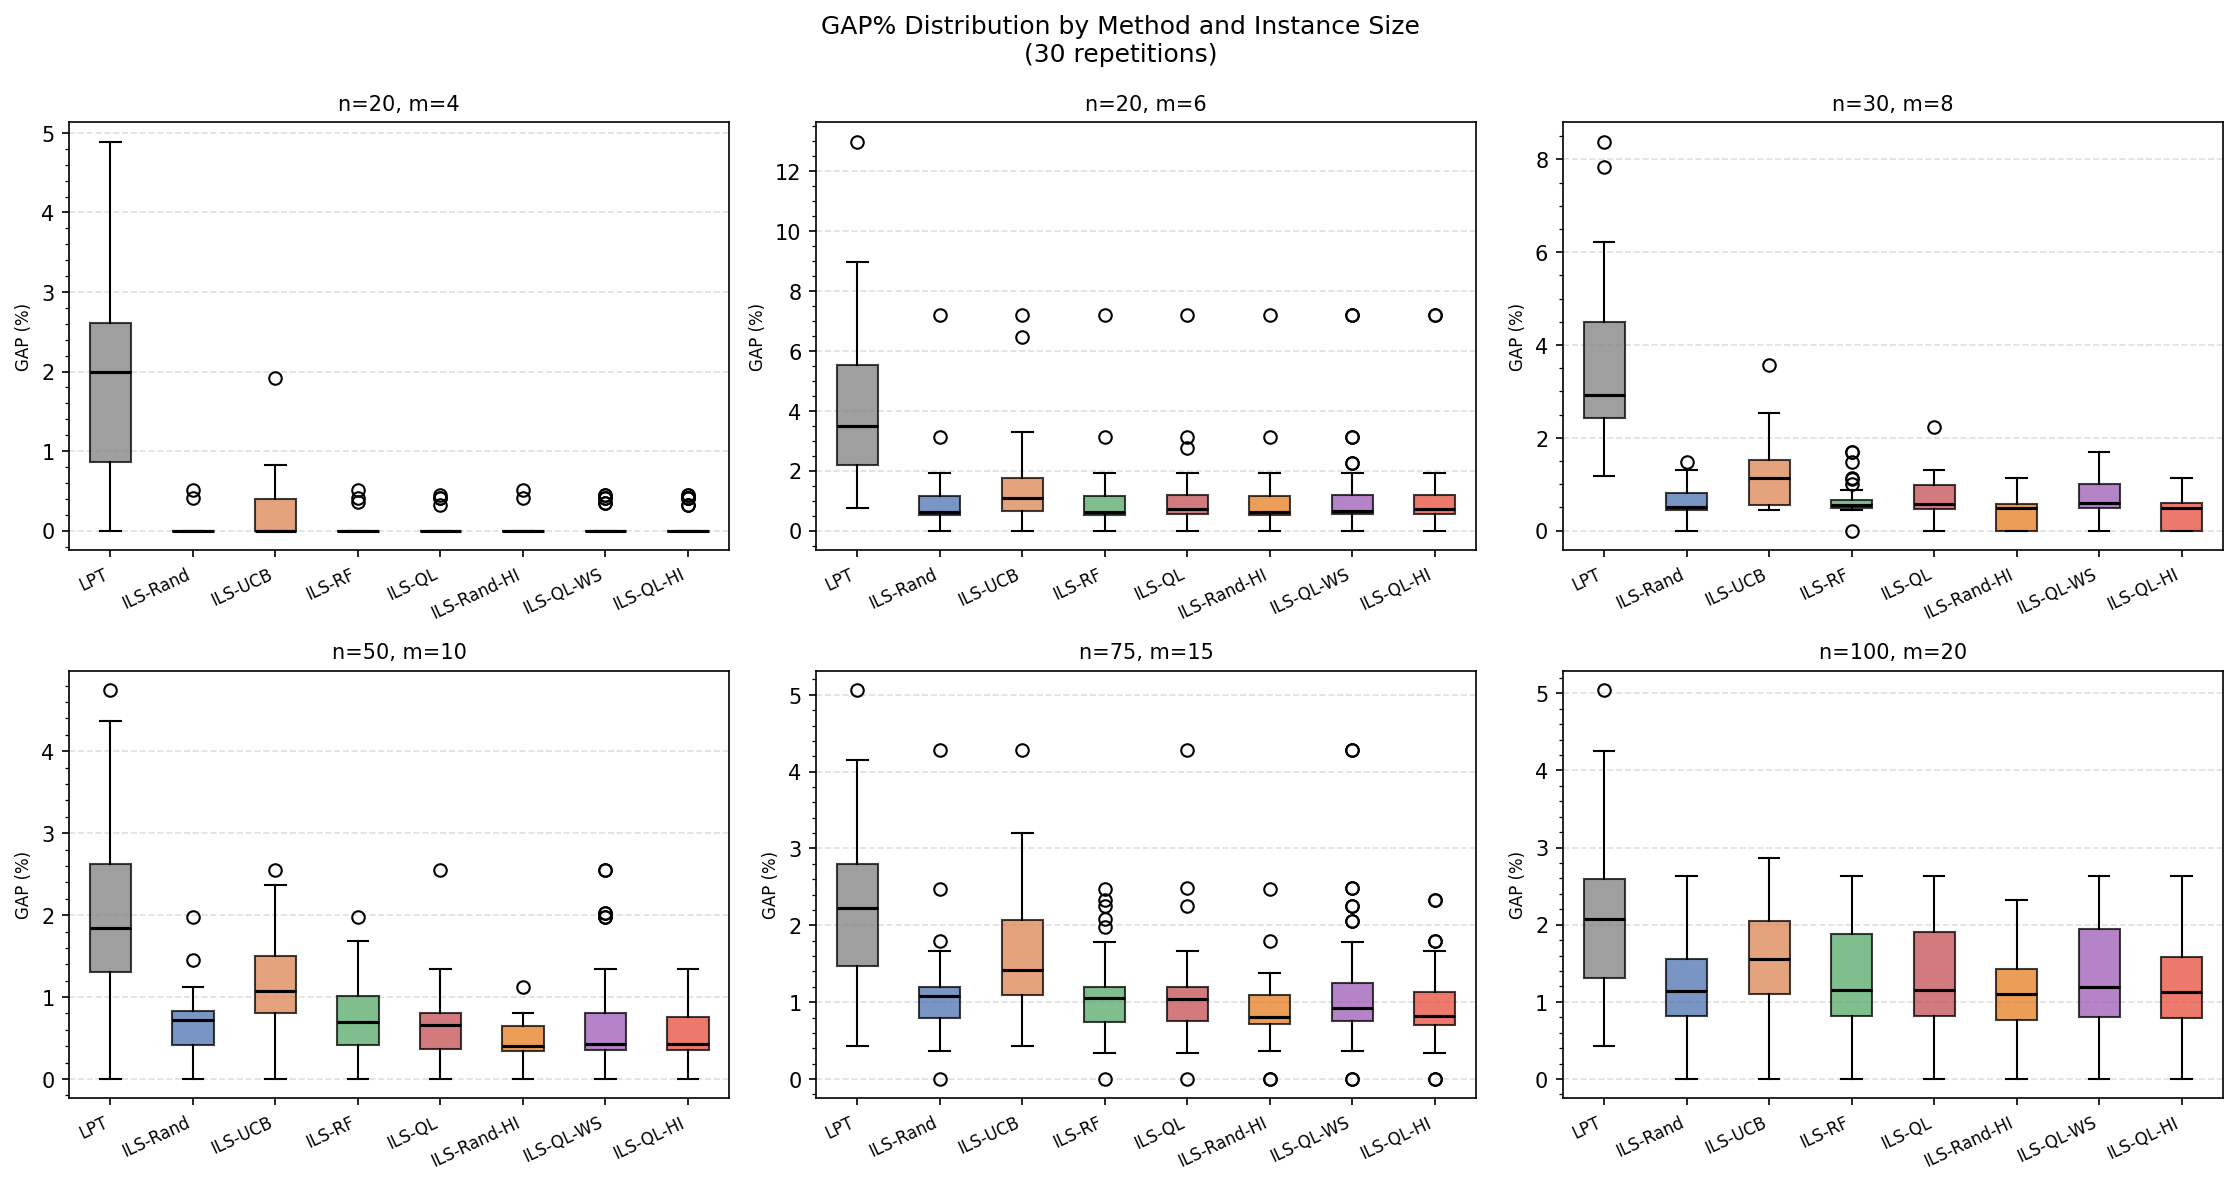
\includegraphics[width=0.92\textwidth]{fig_gap_boxplot.png}
\caption{GAP(\%) boxplots by instance class and method. Each box
         aggregates 30 distinct instances. HI variants omitted for
         clarity.}
\label{fig:boxplot}
\end{figure}

\paragraph{Why UCB underperformed, and why that was an artefact}
In the runs above, UCB1 was fed raw rewards (reductions of the makespan
in units of the processing times), whereas the analysis of UCB1
assumes rewards in $[0,1]$. With rewards that are zero in almost every
step and large when they occur, the exploration bonus either dominates
the mean (small rewards) or vanishes (large ones), so the behaviour
depends on the scale of the instance: the raw selector is not scale
invariant. The mean number of improvements per run for ILS-UCB was
$1.0$--$2.6$, against $2.1$--$3.8$ for ILS-Rand. The earlier
explanation (premature commitment to a suboptimal operator) is
therefore withdrawn. Re-running UCB1 with each reward divided by the
largest reward observed so far ($N=100$ instances in each of the 12
classes; hypotheses and decision rules fixed in the research diary before
the runs), the normalised variant is far better than the raw one (pooled
GAP $-23.7\%$, $p_{\mathrm{holm}}=8\times10^{-66}$), indistinguishable
from ILS-QL on the six original classes ($p=0.78$) and not significantly
different from random selection ($+3.9\%$, $p=0.069$). In IG, raw and
normalised UCB1 do not differ ($p=0.69$).

\paragraph{A wider ablation confirms the pattern, and confirms that
the operator set -- not the selection mechanism -- is what matters}
The same original protocol was later extended with three further
classical AOS mechanisms already cited in this study -- Probability
Matching \citep{Davis1989}, Adaptive Pursuit \citep{Thierens2005}, and
an on-policy SARSA agent \citep{RummeryNiranjan1994} reusing the same
81-state representation and reward signal as ILS-QL, differing only
in its update rule -- together with three further single-operator
controls, \texttt{ils\_op2\_only} through \texttt{ils\_op4\_only},
complementing \texttt{ils\_op1\_only} above. Aggregated over the same
six classes and 30 instances each ($N=180$ per method), the three new
AOS mechanisms cluster in the same narrow band as the methods already
discussed (mean GAP: Probability Matching $0.796\%$, Adaptive Pursuit
$0.796\%$, SARSA $0.831\%$, against $0.782$--$0.827\%$ for
ILS-Rand/RF/QL above) -- a third, independent replication of the
finding that the specific AOS mechanism chosen barely matters for
this problem, now spanning six mechanisms (uniform random, UCB1,
Q-Learning, a random-forest predictor, Probability Matching and
Adaptive Pursuit) and both major TD-learning paradigms (Q-Learning is
off-policy; SARSA is on-policy). The three additional single-operator
controls, by contrast, are markedly worse than every multi-operator
method (\texttt{ils\_op2\_only} $1.390\%$, \texttt{ils\_op4\_only}
$1.408\%$, \texttt{ils\_op3\_only} $2.584\%$), confirming, alongside
\texttt{ils\_op1\_only} above, that ILS's effectiveness genuinely
depends on having the full four-operator set available.
\texttt{ils\_op3\_only} in particular ties LPT's own makespan exactly
in $160$ of the $180$ instances tested and is never worse than LPT,
improving on it only occasionally and modestly in the remainder -- a
weak but not literally inert operator in isolation, and the reason
its aggregate GAP sits so close to LPT's own ($2.744\%$).

\subsection{Statistical Analysis}
\label{sec:stats}

Table~\ref{tab:wilcoxon} reports $p$-values from the paired Wilcoxon
signed-rank test (two-sided, $n{=}30$ paired observations) for ILS-QL
against four competitors. $p<0.05$ indicates a statistically
significant difference.

\begin{table}[ht]
\centering
\caption{Wilcoxon test $p$-values: ILS-QL vs.\ each competitor.
         \textbf{Bold}: significant difference ($p < 0.05$).
         Headers indicate $(n \times m)$.}
\label{tab:wilcoxon}
\renewcommand{\arraystretch}{1.15}
{\footnotesize
\setlength{\tabcolsep}{4pt}
\begin{tabular}{@{}lcccccc@{}}
\toprule
Competitor
  & $20{\times}4$  & $20{\times}6$  & $30{\times}8$
  & $50{\times}10$ & $75{\times}15$ & $100{\times}20$ \\
\midrule
ILS-Rand
  & 0.715 & 0.285 & 0.300 & 0.427 & 0.678 & 0.075 \\
ILS-Rand-HI
  & 0.715 & 0.169 & \textbf{0.010}
  & \textbf{0.028} & 0.064 & \textbf{0.002} \\
ILS-RF
  & 0.893 & \textbf{0.046} & 0.553 & 0.470 & 0.955 & 0.500 \\
ILS-UCB
  & \textbf{0.003} & \textbf{0.008} & \textbf{0.000}
  & \textbf{0.000} & \textbf{0.000} & \textbf{0.003} \\
\bottomrule
\end{tabular}}
\end{table}

ILS-QL shows no statistically significant difference from ILS-Rand in
any of the six configurations ($p > 0.07$), nor from ILS-RF in
five of the six. In the original runs ILS-QL appeared to outperform
ILS-UCB in all six configurations ($p \leq 0.008$); this was an artefact
of the raw-reward UCB1 (see above), and with normalised rewards the two
are indistinguishable.

The isolation-control comparison (ILS-Rand-HI vs.\ ILS-QL) reveals
that the extended budget significantly outperforms ILS-QL for
$n \geq 30$ ($p \leq 0.028$), whereas the difference between ILS-QL-HI
and ILS-QL-WS is not statistically significant. These results suggest
that, for the PMSP under the budgets evaluated, the number of
iterations tends to be a more impactful factor than the sophistication
of the AOS mechanism.

\subsection{Learned Policy Analysis}
\label{sec:policy}

To assess what the Q-Learning agent internalised, the greedy policy
$\pi(s) = \arg\max_a Q(s,a)$ was extracted from the Q-tables averaged
over 30 runs per class and computed the fraction of the 81 states in
which each operator is greedy-optimal (Table~\ref{tab:policy}).

\begin{table}[ht]
\centering
\caption{Fraction of states (\%) in which each operator is
         greedy-optimal, averaged over 30 Q-tables per instance
         class.}
\label{tab:policy}
\renewcommand{\arraystretch}{1.15}
{\footnotesize
\begin{tabular}{@{}lrrrr@{}}
\toprule
Class & Op1 (inter-swap) & Op2 (reinsert) & Op3 (intra-swap) & Op4 (block-move) \\
\midrule
$n{=}20$, $m{=}4$   & 87.7 & 7.4 & 0.0 & 4.9 \\
$n{=}20$, $m{=}6$   & 93.8 & 1.2 & 0.0 & 4.9 \\
$n{=}30$, $m{=}8$   & 90.1 & 6.2 & 0.0 & 3.7 \\
$n{=}50$, $m{=}10$  & 96.3 & 2.5 & 0.0 & 1.2 \\
$n{=}75$, $m{=}15$  & 95.1 & 2.5 & 0.0 & 2.5 \\
$n{=}100$, $m{=}20$ & 96.3 & 2.5 & 0.0 & 1.2 \\
\bottomrule
\end{tabular}}
\end{table}

A striking, consistent pattern emerges across all classes: Op1
(inter-machine swap) is the greedy-optimal operator in $87$--$96\%$
of states, and the proportion of Op1 grows with instance size. Op3
(intra-machine swap) is \emph{never} preferred. The preference for
Op1 appears invariant to search phase ($f_3$), stagnation level
($f_4$) and solution quality ($f_1$): the operator ranking is
nominally identical across the 81 feature combinations -- but, as
discussed below, most of these combinations are in fact never
visited within a run, which is consistent with either a genuine
invariance or an initialisation artefact.

This finding is structurally interpretable: makespan depends directly
on machine loads, so inter-machine transfers (Op1, Op2, Op4) reduce
$C_{\max}$ by redistributing load, while intra-machine swaps (Op3)
only reorder tasks on the same machine without affecting $C_i$. The
Q-Learning agent empirically identifies this structural property
without prior knowledge, converging to a policy that concentrates
search on inter-machine moves.

\paragraph{Methodological caveat: how much of this finding is real?}
Table~\ref{tab:policy} was computed over Q-tables trained from
scratch (zero initialisation) in a single run per instance -- the
same protocol used by all methods in this study. A follow-up
investigation revealed two facts that qualify this finding. First,
across 12 sampled standard Q-tables, only $21.5$ of the 81 states on
average ($26.5\%$) are visited even once during an entire run; for
states never visited, the corresponding Q-table row remains exactly
zero, and NumPy's \texttt{argmax} tie-break systematically favours
the action at index $0$ (Op1) -- an implementation artefact, not a
learned preference. Second, initialising the Q-table with small
uniform noise (eliminating the artificial tie-break) and aggregating
$30$--$100$ training episodes before freezing the policy for
evaluation, in two reanalysed classes ($n{=}20,m{=}4$ and
$n{=}50,m{=}10$), makes the preference distribution across the four
operators substantially more balanced -- for example, at
$n{=}50,m{=}10$: Op1 in 21 states, Op2 in 28, Op3 in 14 and Op4 in 18,
of 81 -- with Op2 (reinsertion), not Op1, emerging as the most
frequently preferred operator. Notably, state coverage does not grow
beyond $\sim 18$--$24$ of 81 even aggregating up to 100 training
episodes, suggesting that most of the nominal state space is
dynamically unreachable by the ILS search trajectory -- a structural
limitation of the state design, not merely of training budget. The
corrected protocol has not been extended to the other four original
classes (it is listed as future work in
Section~\ref{sec:conclusions}); the numbers in
Table~\ref{tab:policy} reflect the original methodology (cold-start,
zero initialisation) and should be interpreted in light of this
caveat.

Figure~\ref{fig:heatmap} presents the heat map of the learned policy
(original protocol, cold-start) for class $n{=}30$, $m{=}8$; in light
of the caveat above, this map should be read as a portrait of the
policy under the original protocol, not as independent confirmation
of a structural property of the PMSP.

\begin{figure}[ht]
\centering
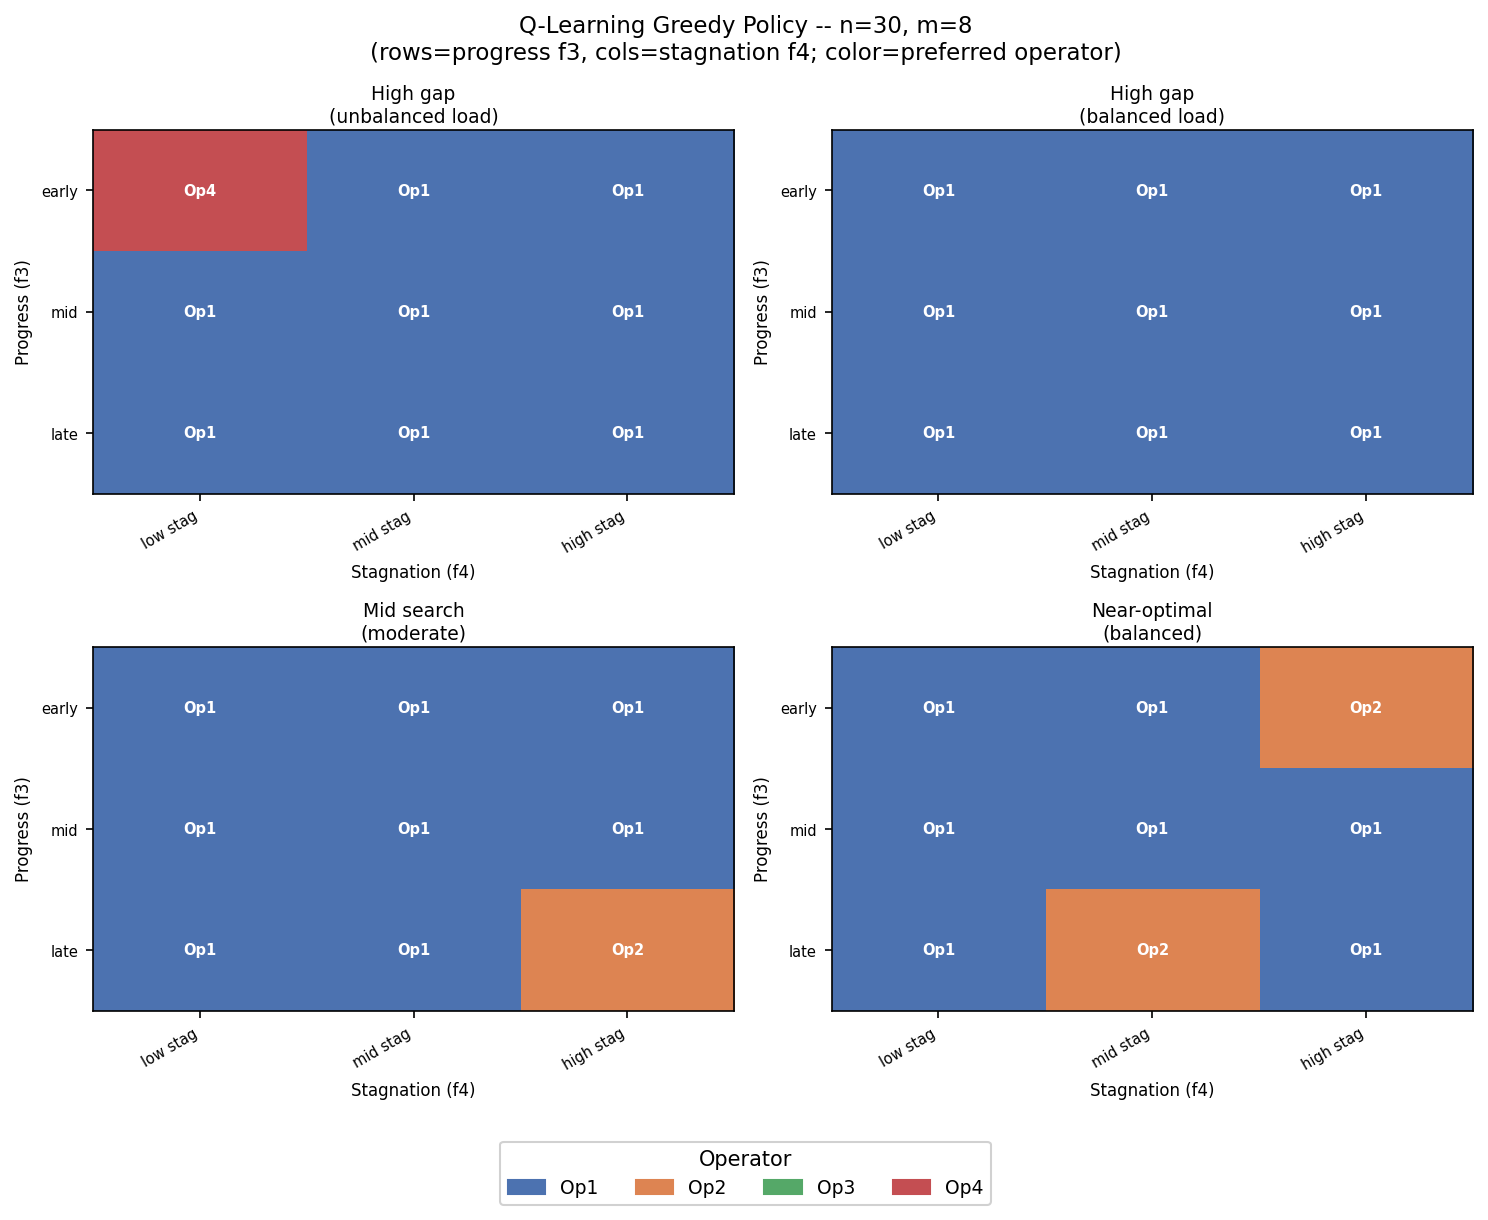
\includegraphics[width=0.85\textwidth]{fig_policy_heatmap.png}
\caption{Heat map of the greedy policy (original protocol,
         cold-start) for class $n{=}30$, $m{=}8$: colour indicates
         the greedy-optimal operator at each state ($f_1 \times f_2$
         for different combinations of $f_3$ and $f_4$). See the
         methodological caveat in the text regarding the influence of
         unvisited states on this visualisation.}
\label{fig:heatmap}
\end{figure}

The near-constant policy (under the original protocol) was also
offered as an explanation for the statistical equivalence between
ILS-QL and ILS-Rand: under this policy, Op1 would be selected
$\approx 90\%$ of the time; under random selection, only $25\%$. This
raised a testable hypothesis -- that an ILS restricted to Op1 alone
would achieve comparable performance, with lower overhead -- which was
tested directly with an additional \texttt{ils\_op1\_only} selector
(Section~\ref{sec:experiments}). The result \textbf{refutes} this
hypothesis: ILS-Op1-only achieved a worse mean GAP ($0.889\%$) than
every multi-operator method at the same budget (ILS-Rand: $0.782\%$;
ILS-RF: $0.812\%$; ILS-QL-WS: $0.825\%$; ILS-QL: $0.827\%$). That is,
even though adaptive selection itself does not outperform random
selection, the availability of the other operators matters --
probably through the ILS perturbation phase, which draws among all
four operators independently of the main selector. This is consistent
with the caveat above: the dominance of Op1 in the learned
\emph{greedy} policy does not imply that the other operators are
dispensable in the algorithm's full dynamics.

\subsection{Isolation Control: Budget versus Learning}
\label{sec:isolation}

The comparison between ILS-Rand-HI and ILS-QL-HI (same extended
budget, different AOS strategies) isolates the contribution of
learning. ILS-Rand-HI achieved a lower mean GAP than ILS-QL-HI in all
six configurations (Table~\ref{tab:results}), with significant
differences for $n \geq 30$ ($p \leq 0.028$, Table~\ref{tab:wilcoxon}).

This indicates that the Q-Learning agent's exploration overhead
(non-Op1 actions taken during the $\varepsilon$-greedy phase) tends to
be mildly detrimental when a dominant operator already exists and the
budget is still moderate. In other words, when the agent's policy
converges strongly to a single operator (Section~\ref{sec:policy} --
with the methodological caveat discussed there about how much of this
is structural versus an initialisation artefact), the cost of
learning that preference competes with the benefit of simply running
more iterations of random search.

This result has a methodologically relevant implication for the AOS
community: experiments that compare only fixed-budget variants may
mask the effect of learning. The isolation control proposed here
allows the two effects to be discriminated cleanly -- the same logic
that, extended to \texttt{ig\_ql}, motivated
Section~\ref{sec:f3f4-ablation}.



% =====================================================================
\section{ILS framework and variants}
\label{sec:ils-framework}
\subsection{ILS framework}

ILS (Algorithm~\ref{alg:ils}) starts from an LPT solution and iterates
for $T$ steps.
At each step, the AOS module selects one of the four neighbourhood
operators, which is then applied under best-improvement local search.
After a fixed number (50) of consecutive iterations without
improvement, a random perturbation (3 random
moves) restarts the search from the best incumbent.
The best result over the $T$ iterations is returned.

\begin{table}[ht]
\centering
\caption{The four neighbourhood operators used in ILS.}
\label{tab:operators}
\begin{tabular}{@{}clp{7.5cm}@{}}
\toprule
\textbf{Op} & \textbf{Name} & \textbf{Description} \\
\midrule
Op1 & inter-swap    & Swaps two jobs between distinct machines. \\
Op2 & reinsert      & Moves a job from the most loaded to the least loaded machine. \\
Op3 & intra-swap    & Swaps two jobs on the same machine (does not change $C_i$). \\
Op4 & block-move    & Transfers a contiguous block of jobs between two machines. \\
\bottomrule
\end{tabular}
\end{table}

\begin{algorithm}[tb]
\caption{ILS with AOS for PMSP}
\label{alg:ils}
\begin{algorithmic}[1]
\REQUIRE Jobs $\mathcal{J}$, machines $\mathcal{M}$, iteration budget $T$, AOS module
\STATE $x \leftarrow \mathrm{LPT}(\mathcal{J},\mathcal{M})$; $x^{*} \leftarrow x$; $\mathrm{stag} \leftarrow 0$
\FOR{$t = 1, \ldots, T$}
\STATE $s \leftarrow \mathrm{encode}(x, t, T)$
\STATE $a \leftarrow \mathrm{AOS}(s)$
\STATE $x' \leftarrow \mathrm{BestImprovement}(x,\, \mathrm{Op}_a)$
\STATE $r \leftarrow C_{\max}(x) - C_{\max}(x')$
\STATE Update AOS with $(s, a, r)$; update $x$, $x^{*}$, $\mathrm{stag}$
\IF{$\mathrm{stag} \geq \mathrm{threshold}$}
\STATE $x \leftarrow \mathrm{Perturb}(x^{*})$; $\mathrm{stag} \leftarrow 0$
\ENDIF
\ENDFOR
\RETURN~$x^{*}$
\end{algorithmic}
\end{algorithm}

Table~\ref{tab:operators} describes the four operators.
Note that Op3 (intra-swap) can never improve the makespan, since it
reorders jobs on the same machine without changing its load.
Its inclusion serves as a structural control: an effective AOS should
learn to avoid it.


\subsection{ILS method variants}
\label{sec:variants}

\paragraph{ILS-QL-WS (\textit{warm-start})}
Before optimising each instance, the Q-table is pre-trained on a batch
of random instances of similar size.
This biased initialisation can accelerate early convergence, reducing
the purely exploratory phase.
The pre-trained Q-table is shared across all runs of the same instance
class.

\paragraph{ILS-QL-HI and ILS-Rand-HI (\textit{high-iteration})}
Both variants receive an extended iteration budget, $1.5$ to
$4{\times}$ the base budget, scaled by instance size: from 1\,500
iterations for $n{=}20$ up to 4\,000 for $n{=}100$, $m{=}20$.
ILS-Rand-HI uses random operator selection under this extended budget,
serving as an \emph{isolation control}: any performance difference
between ILS-Rand-HI and ILS-QL-HI can be attributed to the AOS
strategy rather than to the available budget.

\paragraph{AOS baselines}
Besides ILS-Rand (uniform random selection), two further baselines are
evaluated: ILS-UCB, based on the UCB1 algorithm with $c{=}\sqrt{2}$,
treating operators as bandit arms; and ILS-RF, which trains an online
Random Forest \citep{BreimanRF2001} on the mapping $(s,a) \to r$ to
predict the expected improvement of each operator.


% =====================================================================
\section{Additional robustness experiments and pre-specification record}
\label{sec:robust}

This section reports the experiments run to answer foreseeable reviewer
objections. Each one was specified before it was run: the hypotheses, the
decision rule, the test family and the md5 hashes of the code and of the
data files it reads were written in the research diary, and the analysis
script was frozen. Deviations that had to be made are listed in
Section~\ref{sec:prereg-record}; none was made after seeing a result of
the affected test.

\subsection{Convergence behaviour}
\label{sec:convergence}

Figure~\ref{fig:convergence} plots best-makespan-so-far against
iteration for a single representative run of \texttt{ig\_ql},
\texttt{ils\_ql} and \texttt{sa\_li\_perkins} at three sizes:
$(20,4)$, $(100,20)$ and $(300,20)$, all at the standard budget
$T=1{,}000$.

\begin{figure}[ht]
\centering
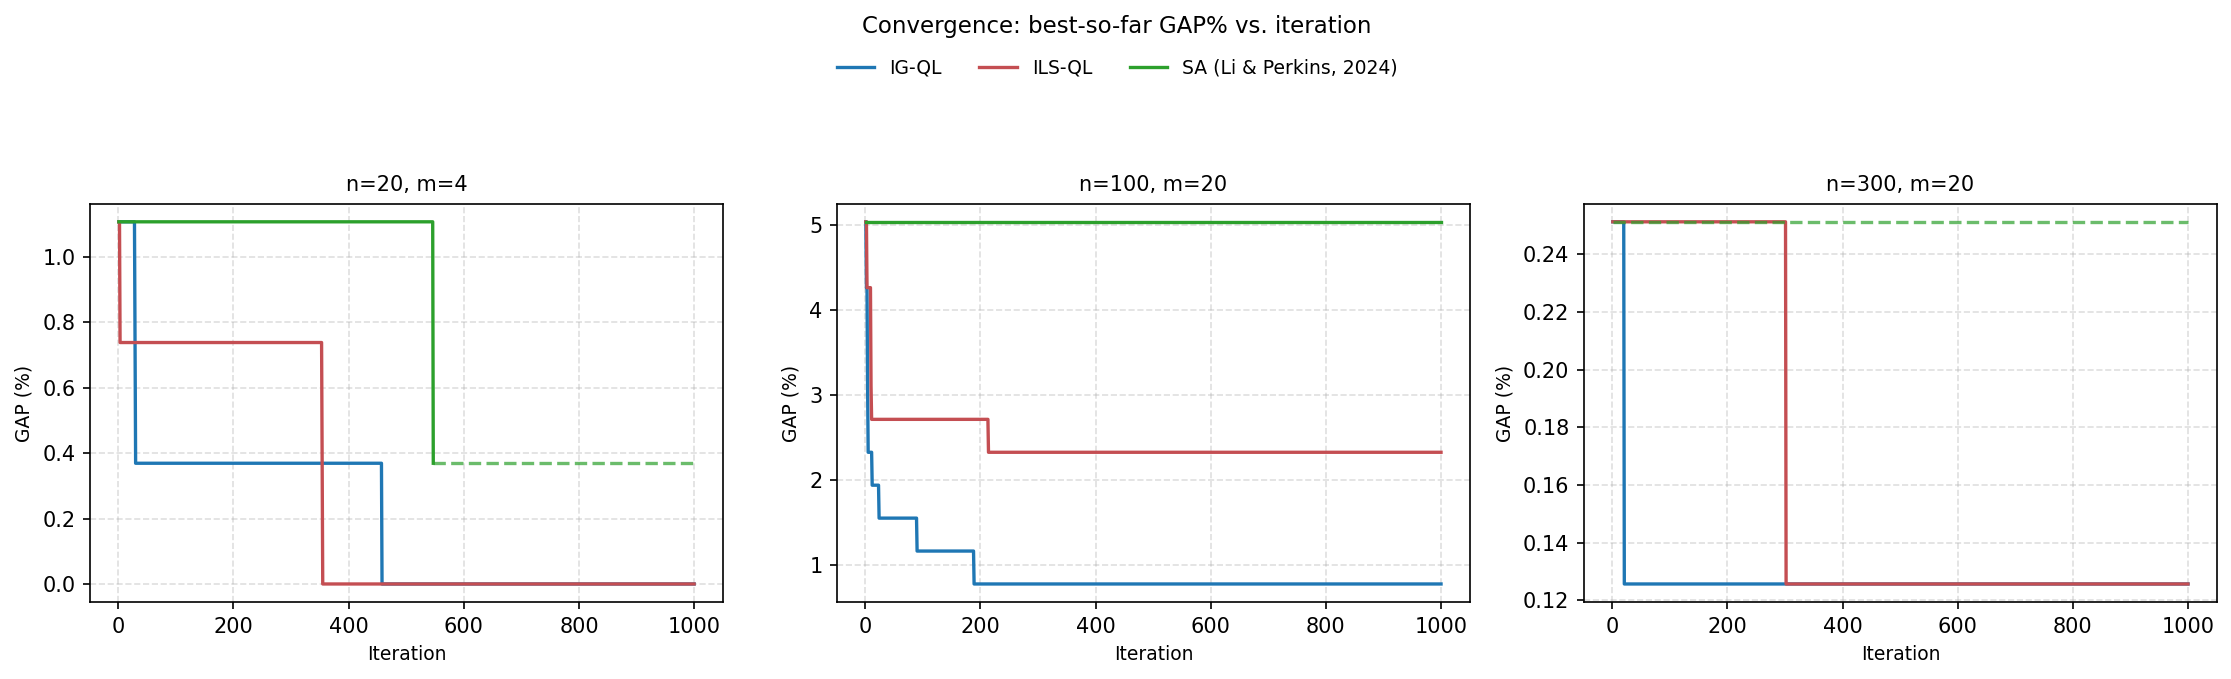
\includegraphics[width=0.95\textwidth]{fig_convergence.png}
\caption{Convergence of best-makespan-so-far (as GAP\% relative to the
         lower bound) against iteration, for \texttt{ig\_ql},
         \texttt{ils\_ql} and \texttt{sa\_li\_perkins}, at three
         representative instance sizes. Dashed segments mark where
         \texttt{sa\_li\_perkins} has already met its own early-stopping
         criterion and the plotted curve is a forward-filled constant,
         not further search.}
\label{fig:convergence}
\end{figure}

\texttt{ils\_ql} typically improves in larger, less frequent steps early
on and then plateaus, consistent with an exhaustive best-improvement
search that quickly exhausts the moves around its current bottleneck
machine (Section~\ref{sec:hybrid}); \texttt{ig\_ql} improves in smaller,
more frequent steps throughout the budget, since its stochastic
destroy-and-reconstruct step never fully exhausts a neighbourhood.
\texttt{sa\_li\_perkins}, faithfully reimplementing the early-stopping
rule of \citet{LiPerkins2024} (halt once the best solution is within
$1.01\times$ of the lower bound), terminates well before the shared
budget in the smaller classes (only $547$ of $1{,}000$ iterations execute
at $(20,4)$) and at $(300,20)$ never executes an iteration: the initial
LPT solution already has a GAP of $0.25\%$, inside the stopping target.
This is a property of the original method, not an implementation defect,
and the dashed extension exists so that the flat segment is not mistaken
for search that found nothing.

\subsection{Seed variance}
\label{sec:seedvar}

All batteries run each method once per instance. To measure the noise this
leaves, all twelve classes were rerun with 20 instances and ten algorithm seeds
each ($9{,}600$ runs; a pilot on three classes with the same design came first).
Table~\ref{tab:s_seed} shows that the share of the GAP variance explained by the
instance has a median of $0.44$--$0.45$ for the IG and $0.72$--$0.74$ for the
ILS, and that the within-instance standard deviation (median $0.13$--$0.14$
percentage points, up to $0.9$ for the ILS at $(60,20)$) is of the same order as
the policy effect itself, which is why per-class single-run tests cannot resolve
it. The pre-specified criterion for the pilot (S1: equivalence to zero within
$\pm0.05\%$ of the policy effect on seed averages) was \emph{not} met
($\bar d=-0.045\%$, 90\% interval $-0.063$ to $-0.027$), because the three
pilot classes happened to have the largest effects. The twelve-class test (S1$'$,
240 instances) gives $\bar d=-0.011\%$ (90\% interval $-0.019$ to $-0.003$,
$p=0.009$): a real effect, and strictly equivalent to zero within $\pm0.05\%$;
only $(30,8)$ detects it individually after correction ($-0.076\%$). Criterion
S2$'$ (the sign of the IG-versus-ILS contrast on seed averages equals that of the
single run, per class, for the random and the Q-Learning variants) was met in
$23$ of $24$ contrasts (the exception is a tie at $(20,4)$); on seed averages the
IG beats the ILS by $0.49\%$ (random variants, 90\% interval $0.39$--$0.60$) and
$0.53\%$ (Q-Learning variants, $0.43$--$0.64$), in $156$ and $168$ of the $240$
instances.

% Auto-generated by analysis/make_tables_supplement_robust.py (Entrada 112)
\begin{table}[t]
\centering
\caption{Seed variance (20 instances $\times$ 10 algorithm seeds per class). Mean GAP (\%), share of the GAP variance explained by the instance (ICC) and mean within-instance standard deviation of the GAP (percentage points).}
\label{tab:s_seed}
{\scriptsize\setlength{\tabcolsep}{4pt}
\begin{tabular}{@{}lrrrrrrrrrrrr@{}}
\toprule
 & \multicolumn{3}{c}{\texttt{ig\_ql}} & \multicolumn{3}{c}{\texttt{ig\_random}} & \multicolumn{3}{c}{\texttt{ils\_ql}} & \multicolumn{3}{c}{\texttt{ils\_random}} \\
\cmidrule(lr){2-4}\cmidrule(lr){5-7}\cmidrule(lr){8-10}\cmidrule(lr){11-13}
Class & GAP & ICC & SD & GAP & ICC & SD & GAP & ICC & SD & GAP & ICC & SD \\
\midrule
$(20,4)$ & 0.009 & -0.02 & 0.029 & 0.029 & 0.15 & 0.051 & 0.071 & 0.21 & 0.100 & 0.034 & 0.12 & 0.067 \\
$(20,6)$ & 0.725 & 0.99 & 0.116 & 0.699 & 0.99 & 0.107 & 1.209 & 0.93 & 0.321 & 1.134 & 0.95 & 0.293 \\
$(30,8)$ & 0.188 & 0.43 & 0.152 & 0.265 & 0.43 & 0.165 & 0.742 & 0.29 & 0.372 & 0.659 & 0.29 & 0.300 \\
$(40,5)$ & 0.042 & 0.46 & 0.039 & 0.041 & 0.42 & 0.042 & 0.038 & 0.46 & 0.037 & 0.037 & 0.40 & 0.040 \\
$(50,10)$ & 0.310 & 0.45 & 0.149 & 0.317 & 0.45 & 0.172 & 0.561 & 0.59 & 0.205 & 0.502 & 0.51 & 0.200 \\
$(60,20)$ & 0.882 & 0.46 & 0.315 & 0.839 & 0.47 & 0.283 & 4.400 & 0.54 & 0.893 & 4.392 & 0.56 & 0.913 \\
$(75,15)$ & 0.555 & 0.46 & 0.171 & 0.590 & 0.47 & 0.160 & 0.970 & 0.63 & 0.275 & 0.934 & 0.63 & 0.278 \\
$(100,20)$ & 0.709 & 0.42 & 0.155 & 0.743 & 0.37 & 0.186 & 1.208 & 0.85 & 0.140 & 1.201 & 0.89 & 0.125 \\
$(150,30)$ & 0.850 & 0.33 & 0.166 & 0.873 & 0.38 & 0.170 & 1.530 & 0.84 & 0.138 & 1.498 & 0.84 & 0.155 \\
$(150,15)$ & 0.190 & 0.45 & 0.041 & 0.199 & 0.41 & 0.038 & 0.264 & 0.92 & 0.020 & 0.265 & 0.88 & 0.030 \\
$(250,25)$ & 0.184 & 0.78 & 0.030 & 0.184 & 0.80 & 0.029 & 0.221 & 0.99 & 0.005 & 0.222 & 0.99 & 0.005 \\
$(300,20)$ & 0.097 & 0.68 & 0.017 & 0.096 & 0.69 & 0.018 & 0.109 & 0.85 & 0.009 & 0.106 & 0.81 & 0.016 \\
\bottomrule
\end{tabular}}
\end{table}


\subsection{Other processing-time distributions and the hard region}
\label{sec:newdist}

To test whether the findings depend on $U[1,100]$ times, 900 new
instances were generated: six distributions ($U[1,100]$, $U[50,100]$,
$U[1,10^4]$, log-normal with parameters $(3,1)$, a bimodal mixture of
$U[5,25]$ and $U[75,100]$, and a Pareto with shape $1.5$ capped at $1000$)
$\times$ five sizes $(n,m)\in\{(25,10),(60,20),(50,10),(100,10),(200,20)\}$
$\times$ 30 replications; the first two sizes lie in the hard region
$n/m \leq 3$. Table~\ref{tab:s_newdist} summarises the outcome.
Pre-specified hypothesis H1 (the policy is equivalent to random selection
within $\pm0.05\%$) was confirmed: $\bar d=-0.016\%$ for \texttt{ig\_ql}
against \texttt{ig\_random} (90\% interval $-0.027$ to $-0.004$) and
$-0.012\%$ with the strong start; the narrow-range $U[50,100]$ is where
the policy helps most ($-0.03$ to $-0.04\%$). All four tests of the
confirmatory family were confirmed (Holm over four): the a priori dispatch
rule (duplicate ratio $>0.1$ selects IG, otherwise ILS; threshold fixed in
earlier work and never retuned) beats always-\texttt{ig\_ql}
($\bar d=-0.022\%$, $p_{\mathrm{Holm}}=3\times10^{-10}$) and
always-\texttt{ils\_ql} ($-0.263\%$, $p_{\mathrm{Holm}}=2\times10^{-36}$);
IG beats ILS when the duplicate ratio exceeds $0.1$ ($\bar d=-0.30\%$, 726
instances) and ILS beats IG when it does not ($+0.10\%$, 174 instances;
115 against 18 wins). The granularity finding of
Section~\ref{sec:nm-structural} therefore holds outside the distribution
in which it was found.

Three further observations. (i) MULTIFIT is \emph{worse} than LPT on
$U[50,100]$ ($3.68\%$ against $2.48\%$ mean GAP; none of its solutions is
provably optimal), so its strength in Section~\ref{sec:f2-sota} is a
property of wide-range times, not of the algorithm in general; LDM does
well there ($49\%$ provably optimal). (ii) \textsc{IG-QL}$^{+}$ improves on
the best constructive solution in $168$ of the $900$ instances and never
worsens it; it has the lowest GAP in four of six distributions (Pareto and
$U[1,10^4]$ are the exceptions). (iii) In the hard region ($n/m\leq3$)
\texttt{ig\_ql} proves optimality for $72\%$ of the instances, against
$52\%$ elsewhere, but these are the smallest sizes, so the comparison is
confounded with $n$.

% Auto-generated by analysis/make_tables_supplement_robust.py (Entrada 112)
\begin{table}[t]
\centering
\caption{New processing-time distributions (30 instances $\times$ 5 sizes = 150 per distribution). Mean GAP (\%) against the best lower bound available (certified arc-flow bound; classical improved bound when the arc-flow graph exceeded $4\times10^5$ arcs, mostly $U[1,10^4]$), and, in parentheses, the share of provably optimal solutions (\%). ``Dup.'' is the share of instances with duplicate ratio $>0.1$.}
\label{tab:s_newdist}
{\scriptsize\setlength{\tabcolsep}{3.5pt}
\begin{tabular}{@{}lrrrrrr@{}}
\toprule
Distribution & Dup. (\%) & \textsc{MultiFit} & \textsc{LDM} & \textsc{IG-QL} & \textsc{ILS-QL} & \textsc{IG-QL}$^{+}$ \\
\midrule
$U[1,100]$ & 90 & 0.314 (59) & 1.672 (41) & 0.286 (42) & 0.956 (29) & \textbf{0.206} (68) \\
$U[50,100]$ & 99 & 3.679 (0) & 1.421 (49) & 0.174 (41) & 0.703 (31) & \textbf{0.095} (75) \\
$U[1,10^4]$ & 0 & 0.449 (9) & 1.986 (6) & 0.424 (14) & \textbf{0.210} (13) & 0.318 (13) \\
Log-normal & 97 & 0.034 (93) & 0.073 (88) & 0.021 (94) & 0.057 (84) & \textbf{0.009} (98) \\
Bimodal & 98 & 0.136 (61) & 0.340 (76) & 0.080 (75) & 0.307 (51) & \textbf{0.051} (88) \\
Pareto & 100 & 0.343 (79) & 0.479 (81) & \textbf{0.054} (94) & 0.299 (81) & 0.064 (91) \\
\bottomrule
\end{tabular}}
\end{table}


\subsection{IG versus ILS at equal CPU time}
\label{sec:eqcpu}

For equal $T$, an ILS iteration costs more than an IG iteration (up to
$24.8\times$ at $n=300$; Section~\ref{sec:exact-ref}). To check that
the IG-versus-ILS findings are not an artefact of the iteration budget,
IG was given $T_{\mathrm{IG}}=1000\,K(n)$ iterations, with $K$ interpolated
from the measured CPU ratios ($K=1.5$ to $15$ for the Q-Learning variant,
$1.1$ to $6.3$ for the random one) and fixed in advance, on the
fine-grained $U[1,10^4]$ and the coarse $U[1,100]$ instances of the
previous subsection. Table~\ref{tab:s_eqcpu} shows that the ILS advantage
on fine-grained times persists at equal CPU ($\bar d=+0.09\%$ and
$+0.14\%$, $p_{\mathrm{Holm}}\leq10^{-7}$; ILS is ahead at every size from $n=50$, the Q-Learning variant only marginally at $n=60$),
and that the IG advantage on coarse times grows ($-0.70\%$ and $-0.68\%$).
The realised IG/ILS CPU ratio was $0.8$--$1.7$.

% Auto-generated by analysis/make_tables_supplement_robust.py (Entrada 112)
\begin{table}[t]
\centering
\caption{IG versus ILS at approximately equal CPU time (IG receives $T_{\mathrm{IG}}=1000\,K(n)$ iterations, $K$ from the measured CPU ratios; ILS uses $T=1000$). $\bar d$: mean relative makespan difference (\%; negative: IG better). 150 instances per row; Wilcoxon, Holm over the four tests.}
\label{tab:s_eqcpu}
{\scriptsize\setlength{\tabcolsep}{4pt}
\begin{tabular}{@{}llrrrrr@{}}
\toprule
Distribution & Comparison & W/L/T & $\bar d$ (\%) & $r$ & $p_{\mathrm{Holm}}$ \\
\midrule
$U[1,10^4]$ & \texttt{ig\_ql} vs.\ \texttt{ils\_ql} & 21/103/26 & +0.086 & +0.79 & $8.8\times10^{-8}$ \\
$U[1,10^4]$ & \texttt{ig\_random} vs.\ \texttt{ils\_random} & 15/113/22 & +0.138 & +0.82 & $1.7\times10^{-11}$ \\
$U[1,100]$ & \texttt{ig\_ql} vs.\ \texttt{ils\_ql} & 82/6/62 & -0.703 & -0.93 & $4.3\times10^{-14}$ \\
$U[1,100]$ & \texttt{ig\_random} vs.\ \texttt{ils\_random} & 73/8/69 & -0.676 & -0.91 & $2.7\times10^{-12}$ \\
\bottomrule
\end{tabular}}
\end{table}


\subsection{Destruction size and other hyperparameters}
\label{sec:hyper}

$\alpha$, $\gamma$, the $\varepsilon$ decay and the destruction fraction
$d/n$ were varied one at a time around the defaults ($0.1$, $0.9$, $0.995$,
$0.3$) on six classes with 50 instances each (3{,}600 runs). The family of
nine pre-specified tests (Holm) asked whether the Q-Learning policy beats
the matched random control by a practically relevant margin
($\geq0.05\%$) in any setting; it does at $d=0.1n$ ($-0.112\%$,
$p_{\mathrm{Holm}}=2\times10^{-7}$) and $d=0.2n$ ($-0.057\%$,
$p_{\mathrm{Holm}}=0.015$), not at $d=0.4n$ ($-0.037\%$) nor for any value of
$\alpha$, $\gamma$ or the decay (all $|\bar d|\leq0.023\%$, none
significant). The null of the policy is therefore not robust to the
destruction size, although the effect never exceeds $0.11\%$.
Table~\ref{tab:s_hyperd} shows that the default $d=0.3n$ is clearly
suboptimal at larger $n$: $d=0.1n$ cuts the mean GAP of \texttt{ig\_ql}
by a factor of three to four at $(100,20)$ and $(75,15)$ and by more than half at
$(150,30)$, but it hurts at $(20,6)$, where the larger sizes are better. Choosing $d$ by instance size (for instance, by cross-validation on
separate instances) is a natural improvement that was deliberately not
applied, so that no parameter was tuned on the evaluation instances.

% Auto-generated by analysis/make_tables_supplement_robust.py (Entrada 112)
\begin{table}[t]
\centering
\caption{Mean GAP (\%) against the classical lower bound as a function of the destruction size $d/n$ (50 instances per class; $d=0.3n$ is the default used throughout and was never tuned). Bold: best $d$ in each row for each method.}
\label{tab:s_hyperd}
{\scriptsize\setlength{\tabcolsep}{4pt}
\begin{tabular}{@{}lrrrrrrrr@{}}
\toprule
 & \multicolumn{4}{c}{\texttt{ig\_ql}} & \multicolumn{4}{c}{\texttt{ig\_random}} \\
\cmidrule(lr){2-5}\cmidrule(lr){6-9}
Class & 0.1 & 0.2 & 0.3 & 0.4 & 0.1 & 0.2 & 0.3 & 0.4 \\
\midrule
$(20,6)$ & 1.381 & 0.667 & 0.522 & \textbf{0.495} & 1.723 & 0.855 & \textbf{0.513} & 0.548 \\
$(50,10)$ & \textbf{0.148} & 0.149 & 0.262 & 0.378 & 0.212 & \textbf{0.181} & 0.293 & 0.385 \\
$(75,15)$ & \textbf{0.148} & 0.334 & 0.591 & 0.541 & \textbf{0.210} & 0.404 & 0.574 & 0.594 \\
$(100,20)$ & \textbf{0.187} & 0.463 & 0.619 & 0.578 & \textbf{0.278} & 0.503 & 0.726 & 0.614 \\
$(150,30)$ & \textbf{0.338} & 0.752 & 0.839 & 0.664 & \textbf{0.471} & 0.763 & 0.884 & 0.729 \\
$(300,20)$ & 0.133 & 0.092 & 0.084 & \textbf{0.049} & 0.126 & 0.102 & 0.073 & \textbf{0.060} \\
\bottomrule
\end{tabular}}
\end{table}


\paragraph{Budget of the learning-free recipe}
Table~\ref{tab:s_recipe_budget} extends the recipe of the main text (tuned destruction size, start from the best constructive solution, no learning, no local search) to larger budgets on six classes. The trajectories share the seed, so quality is non-increasing in $T$ by construction. The share of provably optimal solutions rises from $75.5\%$ at $T=1{,}000$ to $86.8\%$, $92.7\%$ and $97.5\%$ at $T=4{,}000$, $16{,}000$ and $64{,}000$ (mean GAP $0.099\%$ to $0.009\%$; $100\%$ at $(50,10)$), at a CPU time of $3$--$6$ seconds per run at $T=16{,}000$ and $12$--$24$ seconds at $T=64{,}000$ (parallel runs, indicative). The classes with $n/m\geq10$ are saturated early because the start is already optimal; the saturation point is not reached by $T=64{,}000$ in the four smaller classes (analysis descriptive, specified in the diary, Entry 139).

%% Table~\ref{tab:s_recipe_budget} now lives in the main text (Section 4.3).

\subsection{Certified lower bound: method and validation}
\label{sec:lbaf}

For a capacity $C$ let the nodes be the partial sums $0\leq s\leq C$
reachable by a subset of the processing times, with an arc $s\to s+p$ for
each distinct time $p$ and each reachable $s$, plus loss arcs to node $C$.
The relaxation minimises the flow $z$ from $0$ to $C$ subject to flow
conservation and to using each distinct size $p$ exactly as often as it
occurs: $z^{*}(C)$ is the minimum fractional number of bins of capacity $C$.
If $z^{*}(C)>m$, no schedule has makespan $\leq C$, and $z^{*}$ is
non-increasing in $C$, so LB$^{\mathrm{AF}}$ is found by bisection between
the improved classical bound $\max\{p_{\max},\lceil\sum p/m\rceil,p_{(m)}+p_{(m+1)}\}$
and the best known makespan. Infeasibility is declared only if
$z^{*}(C)>m+10^{-4}$, and if the interior-point solver does not finish in 90 s
nothing is declared, so the bound can only be too weak, never invalid.
Validation: (i) against brute force on random small instances the bound is
valid and at least $85\%$ tight; (ii) on 150 published instances with
optimum proven by the iAF method it exceeded the optimum in none and
equalled it in $148$ ($98.7\%$), with a median time of $0.2$\,s (maximum
$149$\,s); (iii) on the 1{,}200 synthetic instances $903$ were proven optimal,
for $199$\,s of CPU in total. For distributions with very wide ranges
(Section~\ref{sec:newdist}) the graph exceeds $4\times10^{5}$ arcs and
the classical improved bound is used instead.

\subsection{Pre-specification record}
\label{sec:prereg-record}

Table~\ref{tab:s_prereg_all} lists, for every confirmatory analysis of the study,
the diary entry holding its specification (hypotheses, decision rule, test family,
and the md5 hashes of the code and of the data files it reads), and the outcome. The
families are Holm-corrected within themselves; all outcomes, including every
non-confirmation, are listed. Deviations that occurred were decided before any test
result of the affected analysis had been read: (a) the synthetic subset in the
stronger-baselines test has $1{,}130$ rather than $1{,}200$ instances because the stored
$(20,4)$ runs of three methods have 30 replications (a failed coverage assertion
revealed it); (b) the reference rows of the signal test use the available pairs for the
same reason; (c) the exact phase of the new-distributions run skips instances whose
arc-flow graph is too large ($>4\times10^{5}$ arcs, after an initial limit of
$3\times10^{6}$ proved too permissive); (d) two analysis scripts had a type error
that aborted them before producing any output, and were corrected without changing a
hypothesis or a rule (seed variance, twelve classes; the unrelated-machine law). Two
process-pool crashes of the operating system, unrelated to the data, interrupted
runs, which were relaunched from the start or resumed. Deviations in the earlier
analyses, if any, are recorded in their diary entries. The pre-specification is a
dated, hash-stamped diary, not a public registry.

% Quadro global das analises pre-especificadas (Entrada 125). Linhas E124 preenchidas apos a execucao.
\begin{longtable}{@{}p{0.23\textwidth}p{0.06\textwidth}p{0.33\textwidth}p{0.30\textwidth}@{}}
\caption{All pre-specified (confirmatory) analyses of the study, with the verdict under the stated decision rule. Non-confirmations are listed on equal footing.}\label{tab:s_prereg_all}\\
\toprule
Analysis & Diary & Decision rule & Outcome \\
\midrule
\endfirsthead
\toprule
Analysis & Diary & Decision rule & Outcome \\
\midrule
\endhead
Held-out Q-Learning effect (4{,}160 published instances) & 90 & Family-level paired test, three families & Confirmed in B, C, E (small) \\
A priori dispatch (held-out) & 94 & Beats always-IG and always-ILS (Holm 2) & Confirmed (2/2) \\
Granularity factorial & 98 & Direction of IG vs.\ ILS per granularity level & Confirmed (3/3) \\
State recalibration & 98 & Q-Learning vs.\ random with informative state & IG: null; ILS: worse \\
Stronger baselines (P1--P4, two data sets) & 102 & Eight paired tests (Holm 8) & 8/8 confirmed; P1 negligible \\
Headroom and signal & 104 & Headroom $>-0.05\%$; dense and pre-trained reward (Holm 3) & Headroom supported; signal explanation refuted \\
Hyperparameters & 105 & Nine tests vs.\ matched random (Holm 9) & \emph{Not} robust at $d\leq0.2n$ \\
Other distributions & 108 & Equivalence H1; dispatch and granularity (Holm 4) & H1 and 4/4 confirmed \\
Seed variance, three classes & 109 & Equivalence S1; sign agreement S2 & S1 \emph{not} met; S2 met (6/6) \\
Equal CPU time & 110 & ILS advantage on fine times persists (Holm 4) & Persists \\
Destruction size as action space & 114 & Headroom A1; policy A2--A4 (Holm 4) & A1 confirmed; policy captures none (A2 \emph{not} confirmed) \\
Second confirmatory test (2{,}690 new published instances) & 115 & Original and informative state vs.\ random (Holm 6) & 6/6 confirmed; informative state adds nothing \\
Seed variance, twelve classes & 117 & Equivalence S1$'$; sign agreement S2$'$ & Real and strictly equivalent ($-0.011\%$); 23/24 \\
Strong start for both mechanisms & 117 & I1--I3, two data sets (Holm 6) & Confirmed; ILS policy slightly worse (I1) \\
Unrelated machines & 118 & M1--M4 (Holm 4) & M1, M2 confirmed; ILS policy worse; MILP not beaten (M4 \emph{not}) \\
Budget law ($T=100,250$) & 121 & B1--B4 (Holm 4) & B4 (headroom) confirmed; B1--B3 (policy) \emph{not} \\
Destruction size, $T=5000$ and pre-training & 121 & D1--D4 (Holm 4) & D2 confirmed; D1, D3 \emph{not}; D4: validation better \\
Tuned-$d$ + strong start & 121 & E1--E4, two data sets (Holm 8) & 8/8 confirmed \\
Unrelated machines: budget and equal CPU & 121 & RB1--RB4 (Holm 4) & RB2 confirmed; RB1, RB3, RB4 \emph{not} \\
Unrelated machines: fresh instances, ablation & 124 & L1--L6 (Holm 6) & L1 confirmed ($\rho=0.59$); L4 confirmed; L2, L3, L5, L6 \emph{not} (policy gain $-0.07\%$) \\
Hybrid IG with local search ($\mathrm{P}||C_{\max}$) & 124 & P1--P3 (Holm 3) & P1, P2 confirmed (local search adds $0.15\%$; hybrid beats ILS by $0.72\%$); policy P3 \emph{not} ($-0.004\%$) \\
Recipe with local search & 127 & F1--F5, two data sets (Holm 5) & F1, F3, F4, F5 confirmed (equal iterations); F2 (\emph{equal CPU}) \emph{not}: the local search is worse by $0.034\%$ \\
Unrelated machines at $1000\times50$ vs.\ MILP (60\,s) & 127 & G1--G2 (Holm 2) & \emph{Neither} confirmed: the MILP is better ($+2.24\%$, $+0.89\%$) \\
Hybrid IG at equal CPU ($\mathrm{P}||C_{\max}$) & 129 & Q1 (single test) & Q1 significant but negligible ($-0.010\%$; equivalent within $\pm0.05\%$): $93\%$ of the $0.15\%$ was budget \\
Policy at $1000\times50$ ($\mathrm{R}||C_{\max}$), equal CPU & 133 & Q1, Q2 (Holm 2) & \emph{Neither} confirmed (pooled $-0.35\%$, $-0.19\%$); post hoc: $-1.73\%$ in $U[1,100]$, worse than random in two distributions \\
Offline validation vs.\ policy at $1000\times50$ ($\mathrm{R}||C_{\max}$) & 135 & V1--V3 (Holm 3) & V2 confirmed ($-0.46\%$); V1 inconclusive ($-0.14\%$); V3 \emph{not} ($-0.31\%$) \\
External validation, standard $\mathrm{R}||C_{\max}$ benchmark (700 instances) & 137 & B1, B2a, B2b, B3, B4 (Holm 5) & B1 confirmed ($-2.14\%$ at equal CPU); B2a, B2b \emph{not} ($-0.055\%$, $-0.033\%$); B3 confirmed ($\rho=0.74$); B4 confirmed (validation beats the policy by $0.066\%$) \\
LP-started IG, standard $\mathrm{R}||C_{\max}$ benchmark (420 unused instances) & 141 & L1--L3 (Holm 3) & L1 confirmed ($-1.18\%$ at equal CPU); L2 confirmed ($-0.12\%$); L3 \emph{not} ($+0.055\%$); competitiveness criterion met ($0.85\%$, $0.31\%$ at $n=1000$) \\
LP-started IG vs.\ MILP at $1000\times50$ & 143 & M1--M2 (Holm 2) & \emph{Neither} confirmed ($-0.76\%$, $p_{\mathrm{Holm}}=0.72$); GAP $1.09\%$ against $2.04\%$; equal or better in $62.5\%$ \\
Prospective headroom law, destruction size ($\mathrm{R}||C_{\max}$ benchmark, 700 instances) & 145 & D1--D5 (Holm 5) & D1 confirmed ($-0.065\%$); D2--D5 \emph{not}: Q-Learning worse than random ($+0.15\%$), validation beats online ($+0.36\%$) and pre-trained ($+0.25\%$), $\rho=-0.37$ \\
LP-IG + restricted MILP, standard $\mathrm{R}||C_{\max}$ benchmark (420 unused instances) & 149 & S1--S3 (Holm 3) & All confirmed ($-0.49\%$ at similar CPU; $-0.68\%$; $-0.55\%$); GAP $0.25\%$; criterion met overall and per $n$, \emph{not} per type (job-correlated $0.67\%$) \\
Permutation flowshop (third problem), 120 test instances & 152 & P1--P5 (Holm 5) & P2, P4 confirmed (local search $-0.21\%$ at equal CPU; validation beats the agent by $0.16\%$); P1 (IG vs.\ ILS), P3 (agent $+0.14\%$, worse than random), P5 \emph{not} \\
LP-reduced-cost candidates for the restricted MILP, standard $\mathrm{R}||C_{\max}$ benchmark (700 test instances) & 156 & R1--R3 (Holm 3) & All confirmed in sign; R1 negligible ($-0.03\%$); criterion (GAP $\leq0.25\%$; every type $\leq0.5\%$) \emph{not} met ($0.27\%$; $0.64\%$ in $U[10,100]$) \\
\bottomrule
\end{longtable}


\begingroup\scriptsize\setlength{\bibsep}{0pt}
\bibliographystyle{elsarticle-harv}
\bibliography{refs}
\endgroup
\end{document}
